\documentclass[11pt,a5paper,oneside,fontset=none]{ctexbook}
% \documentclass[11pt,a5paper,twoside,fontset=none]{ctexbook}

% font set
\usepackage{fontspec}
\usepackage[T1]{fontenc}
\usepackage[sc]{mathpazo}
\usepackage{anyfontsize}
\setmainfont{Source Serif 4}
\setsansfont{Source Sans 3}
\setmonofont{Menlo}
\setCJKmainfont[BoldFont=黑体-简 中等,ItalicFont=楷体-简 常规体]{宋体-简 常规体}

% colors
\usepackage[dvipsnames]{xcolor}
\definecolor{pku-red}{RGB}{139,0,18}
\usepackage{colortbl}
\newcommand{\light}[1]{\textcolor{Orchid}{#1}}

% environments
\usepackage{array}
\usepackage{caption}
\usepackage[shortlabels,inline]{enumitem}
\usepackage{booktabs}
\usepackage{makecell}
\usepackage{float}
\usepackage{multicol}
\usepackage{etoolbox}
\usepackage{graphicx}
\usepackage{multirow}
\usepackage{inputenx}
\usepackage{subcaption}


\usepackage[normalem]{ulem}

% math package
\let\Bbbk\relax
\usepackage{amsmath}
\usepackage{mathrsfs}
\usepackage{amssymb}
\usepackage{amsfonts}
\usepackage{stmaryrd}
\usepackage{latexsym}
\usepackage{extarrows}
\SetSymbolFont{stmry}{bold}{U}{stmry}{m}{n}


% math theorems
\usepackage{mdframed}
\usepackage[thmmarks,amsmath]{ntheorem}
\newtheorem{construction}{构造}[chapter]
\newtheorem{observation}{观察}[chapter]
\newtheorem{lemma}{引理}[chapter]
\newtheorem{proposition}{命题}[chapter]
\newtheorem{corollary}{推论}[chapter]
\newtheorem{theorem}{定理}[chapter]
\newtheorem{principle}{规则}[chapter]
\newtheorem{hypothesis}{假设}[chapter]
\newtheorem{axiom}{公理}[chapter]
{
\theoremstyle{plain}
\theoremheaderfont{\bfseries}
\theorembodyfont{\normalfont}
\theoremsymbol{\ensuremath{\Box}}
\newtheorem{definition}{定义}[chapter]
}
{
\theoremstyle{plain}
\theoremheaderfont{\bfseries}
\theorembodyfont{\normalfont}
\theoremsymbol{\ensuremath{\Box}}
\newtheorem{example}{例}[chapter]
}
{
\theoremstyle{nonumberplain}
\theorembodyfont{\normalfont}
\newmdtheoremenv{remark}{注. }
\AtBeginEnvironment{remark}{\small}
}
{
\theoremstyle{nonumberplain}
\theoremheaderfont{\bfseries}
\theorembodyfont{\normalfont}
\theoremsymbol{\ensuremath{\Box}}
\newtheorem{proof}{证明. }
}

% chap/section set
\ctexset{
    chapter={format={\raggedright\bfseries\Huge}},
    section={format={\raggedright\bfseries\LARGE},name={\S,}},
    subsection={format={\raggedright\bfseries\large},name={\S,}}
}

% page style set
\usepackage[a5paper,top=2.5cm,bottom=2.5cm,left=2cm,right=2cm]{geometry}
\usepackage{nonumonpart}
\usepackage{setspace}
\setstretch{1.5}

% cleveref
\usepackage{crossreftools}
% \pdfstringdefDisableCommands{%
%     \let\Cref\crtCref
%     \let\cref\crtcref
% }
\usepackage{hyperref}
\hypersetup{
    colorlinks=true,
    linkcolor=pku-red,     
    urlcolor=violet,
    citecolor=BlueViolet,
    pdffitwindow=true,
}
\usepackage[capitalize, nameinlink]{cleveref}

% customize Chinese cref name
\Crefformat{construction}{构造\,#2#1#3}
\Crefformat{part}{第#2#1#3部分}
\Crefformat{chapter}{第#2#1#3章}
\Crefformat{section}{第\,#2#1#3\,节}
\Crefformat{theorem}{定理\,#2#1#3}
\Crefformat{lemma}{引理\,#2#1#3}
\Crefformat{proposition}{命题\,#2#1#3}
\Crefformat{corollary}{推论\,#2#1#3}
\Crefformat{observation}{观察\,#2#1#3}
\Crefformat{definition}{定义\,#2#1#3}
\Crefformat{remark}{注\,#2#1#3}
\Crefformat{example}{例\,#2#1#3}
\Crefformat{figure}{图\,#2#1#3}
\Crefformat{table}{表\,#2#1#3}
\Crefformat{appendix}{附录\,#2#1#3}

% remarks
\newcommand\lhysays[1]{\textcolor{blue}{[lhy: #1]}}

% exercise set
\newenvironment{hint}{% hint
\par\itshape 提示:
}{}

\renewcommand{\theenumii}{\arabic{enumii}}

% plots
\usepackage{tikz}
\usepackage{tikz-cd}
\usetikzlibrary{arrows}
\usetikzlibrary{arrows.meta,positioning,calc,3d}
\usepackage{pgfplots}
\pgfplotsset{compat=newest}
\tikzset{
    punkt/.style={
        rectangle,
        rounded corners,
        draw=black, very thick,
        minimum height=2em,
        inner sep=6pt,
        text centered,
        fill=gray!30
    }
}

% math notations
\newcommand{\LHS}{\mathrm{LHS}}
\newcommand{\RHS}{\mathrm{RHS}}
\newcommand{\Z}{\mathbb{Z}}
\newcommand{\N}{\mathbb{N}}
\newcommand{\R}{\mathbb{R}}
\newcommand{\Q}{\mathbb{Q}}
\newcommand{\C}{\mathbb{C}}
\newcommand{\E}{\mathbb{E}}
\renewcommand{\O}{\mathcal{O}}
\newcommand{\id}{\mathrm{id}}
\DeclareMathOperator*{\Span}{Span}
\DeclareMathOperator*{\im}{Im}
\DeclareMathOperator*{\rank}{rank}
\DeclareMathOperator*{\card}{card}
\DeclareMathOperator*{\grad}{grad}
\DeclareMathOperator*{\argmax}{argmax}
\DeclareMathOperator*{\epi}{epi}
\DeclareMathOperator*{\maximize}{maximize}
\DeclareMathOperator*{\minimize}{minimize}
\renewcommand{\d}{\mathrm{d}}
\newcommand{\Pow}{\mathcal{P}}
\newcommand{\cov}{\mathsf{Cov}}
\newcommand{\var}{\mathsf{Var}}
\newcommand{\Nor}{\mathcal{N}}
\newcommand{\U}{\mathcal{U}}
\renewcommand{\t}{\mathsf{T}}
\newcommand{\T}{\top}
\newcommand{\F}{\bot}
\newcommand{\norm}[1]{\left\|#1\right\|}
\newcommand{\inner}[2]{\left\langle{#1},{#2}\right\rangle}
\newcommand{\e}{\mathrm{e}}
\newcommand{\const}{\mathrm{const}}
\newcommand{\scB}{\mathscr{B}}
\newcommand{\scF}{\mathscr{F}}
\newcommand{\G}{\mathscr{G}}
\newcommand{\Exp}{\mathsf{Exp}}
\newcommand{\DExp}{\mathsf{DExp}}
\newcommand{\Lap}{\mathsf{Lap}}
\newcommand{\calP}{\mathcal P}
\newcommand{\calS}{\mathcal S}
\newcommand{\calF}{\mathcal F}
\newcommand{\calM}{\mathcal M}
\newcommand{\KL}{\mathrm{KL}}
\newcommand{\ReLU}{\mathsf{ReLU}}
\newcommand{\val}{\mathsf{val}}

\DeclareSymbolFont{symbolsC}{U}{txsyc}{m}{n}
\DeclareMathSymbol{\strictif}{\mathrel}{symbolsC}{74}
            
\title{\bfseries\Huge 标题title}
\author{\itshape\Large 作者 author}
\date{\today}

\includeonly{Chapters/Markov-chain/contents}

\begin{document}
\frontmatter
\pagestyle{empty}
\maketitle
\cleardoublepage
\setcounter{page}{1}
\chapter{前言}
\tableofcontents
\mainmatter
\pagestyle{plain}

\part{AI的逻辑}\label{part:AI-logic}
\chapter{合情推理}\label{chap:plausible-reasoning}


\section{回顾:命题逻辑的演绎推理}

\emph{命题逻辑}\index{命题逻辑}的命题公式由如下定义递归形成
\begin{itemize}
    \item 命题变元$p,q,r,\dots$是命题公式.
    \item 如果$\phi$和$\psi$是命题公式,那么$(\neg\phi)$,$(\phi\vee\psi)$,$(\phi\wedge\psi)$,$(\phi\leftrightarrow\psi)$和$(\phi\to\psi)$都是命题公式.
\end{itemize}
例如,$(p\vee(q\to r))$是命题公式,但是$p\vee\vee q$不是. 

$\neg,\vee,\wedge,\leftrightarrow,\to$被称为\emph{连接词}\index{连接词},$\neg$被称为\emph{否定},$\vee$被称为\emph{析取},$\wedge$被称为\emph{合取},$\leftrightarrow$被称为\emph{双向蕴含},$\to$被称为\emph{蕴含}. 在不产生混淆的时候也会省略括号. $A\wedge B$也常写作$AB$,$\neg A$也常写作$\overline{A}$.

命题逻辑最重要的问题是:\emph{什么样的公式是真的?}给定一个公式集$\Gamma$,对一个公式$\phi$,我们有两种真的概念:
    \begin{itemize}
        \item 语义:$\Gamma\models \phi$.
        \item 语型:$\Gamma\vdash \phi$.
    \end{itemize}

首先看语义。每一个命题变元可以赋值真假:$\T$(真)或$\F$(假). 对于一般公式,可以利用真值表递归地定义公式的真假赋值. 例如,$p\to q$的真值表为
        \[\begin{array}{cc|c}
        p&q&p\to q\\\hline
             \T&\T&\T  \\
             \T&\F&\F  \\
             \F&\T&\T  \\
             \F&\F&\T  \\
        \end{array}\]
符号$\Gamma\models\phi$意味着对任意赋值,只要$\Gamma$全为真,$\phi$就为真.


然后再看语型。推导规则(即语法)描述了从一些公式出发如何得到另外一些公式. 语法推导的形式是
    \[\begin{array}{c}
         \phi\quad\phi\to\psi  \\\hline
         \psi
    \end{array}\]
横线上方的称为\emph{前提}\index{前提},横线下方的称为\emph{结论}\index{结论}. 上面的推导法则被称为\emph{肯定前件}\index{肯定前件}(MP)\index{MP},是三段论的基础.

语法推导可以引入新的连接词,例如
    \[\begin{array}{c}
         \phi\quad\psi  \\\hline
         \phi\wedge\psi
    \end{array}\]
也可以消除连接词,例如
    \[\begin{array}{c}
         \phi\wedge\psi  \\\hline
         \phi
    \end{array}\]
在给定一组推导法则下,我们就可以根据规则来推演命题,这就是\textbf{演绎推理}\index{演绎推理}.

例如,将\emph{归谬法}(RAA)加入推导法则:将$\neg\phi$作为前提,得到了结论$\F$,那么可以推出$\phi$才是结论. 写作
    \[\begin{array}{c}
         [\neg\phi]  \\
         \vdots\\
         \F\\\hline
         \phi
    \end{array}\]
方括号表示假设$[\neg\phi]$是前提,省略号表示推导的中间步骤. 我们就可以得到反证法. 

记号$\Gamma\vdash\phi$的意思是以$\Gamma$作为前提,依据推导法则,可以得到$\phi$作为结论. 从前提出发,按照法则,得出结论的过程,即称谓\emph{演绎推理}\index{演绎推理}. 命题逻辑的主要定理是
\begin{theorem}[完备性定理]\index{完备性定理}
对任意公式集$\Gamma$和任意公式$\phi$,
\[\Gamma\models\phi\iff\Gamma\vdash\phi.\]
\end{theorem}
推论:检验一个演绎推理的正确性可以用真值表完成.

如果$\models \phi$,那么称$\phi$为\emph{重言式}\index{重言式}. 重言式即是不需要加任何假设也一定成立的公式,表明了这一推理逻辑所包含的``正确的废话''. 如果$\psi\leftrightarrow\phi$是重言式,我们就说$\psi,\phi$是\emph{等值}的\index{等值}. 等值的公式在演绎推理中起着相同的作用. 例如:$p\to q$与$\neg q\to\neg p$是等值的,所以证明一个定理也可以去证明它的逆否命题.


\section{合情推理的数学模型}

现在我们从演绎推理过渡到合情推理。生活中的推理并不总是演绎推理. 走在北大校园里,看到有人突然倒地不起,一个合理的第一反应是,\emph{他突发疾病了}. 在常识的意义下,这是一种合理的推理. 我们来仔细分析一下这个推理的过程.

演绎推理包含两个\emph{强三段论}\index{三段论!强~}:
    \[
        \begin{array}{c}
            \begin{array}{c}  
                A \to B \\ A\text{ 是真的} \\ \hline B\text{ 是真的}
            \end{array} 
            \qquad \qquad 
            \begin{array}{c}  
                A \to B \\ B\text{ 是假的} \\ \hline \text{A是假的}
            \end{array}
        \end{array} 
    \]
具体到上面的例子,$A$是``突发疾病'',$B$是``突然倒地不起''. 因此演绎推理应该是:因为突发疾病,所以突然倒地不起.

然而,我们实际上作出的推理形如:因为突然倒地不起,所以更可能突发疾病. 这是一个\emph{弱三段论}\index{三段论!弱~}:,数学上写作 
        \[
        \begin{array}{c}
            \begin{array}{c}  
                A \to B \\ B\text{ 是真的} \\ \hline A\text{ 变得更合理}
            \end{array} 
        \end{array} 
    \]
虽然我们不能得知$A$的真假,但是根据已有的事实$B$,我们可以得到$A$的合理性. 这样没有严格真假的推理模式就是\emph{合情推理}\index{合情推理}.


再次考虑同样的问题,走在北大校园里,看到有人突然倒地不起,你的第一反应是?
    \begin{itemize}
        \item 选项1:他突发疾病了.
        \item 选项2:他接到情报有一枚来自俄罗斯的导弹意外偏航,马上要落在北京,他正在躲避.
    \end{itemize}
虽然选项1和选项2都是可能的,但是他们的合理程度并不同. 这里产生了一个自然的问题:如何刻画不同推理的合理程度?为此,我们引入似然的概念。


\subsection{似然,合情推理的原则}

用符号$A|B$表示当$B$已知(或假设)为真时,命题$A$合理程度的非负实数度量. 如果$A|B$是一个度量,那么任意非负函数$f(A|B)$也会是一个度量,因此$A|B$还不是一个唯一的数学概念。因此,我们现在称$A|B$为以$B$为假设时命题$A$的\emph{似然}\index{似然}. 似然不能定义在任意两个命题之间,只有有合理的关联的命题才能定义似然.

合情推理的原则实际表明了似然之间的关系. 给定相同的假设,似然应该保持命题逻辑中的等值命题. 例如:
    \begin{itemize}
        \item $(A\vee B) | C=(B\vee A) | C$.
        \item $(AB)C|D=A(BC)|D$.
        \item $\neg\neg A|B=A|B$.
    \end{itemize}

考虑从$C$出发推出$AB$为真. 一种可能的推理方法是先推断出$A$为真,然后在$A$为真的前提下,推断出$B$为真. 所以似然$AB|C$应该取决于这两段推理的似然,即$A|C$和$B|AC$,因此存在函数$F$满足
    \[
        AB|C=F(A|C,B|AC).
    \]
然而,这并不能写成$AB|C = F(B|C, A|C)$,考虑$A$是指小明的左眼是蓝色的,$B$是指小明的右眼是棕色的. $A|C$和$B|C$都可以很合理,但$AB|C$则几乎不可能发生.

我们定义的$F$具有如下性质:
\begin{theorem}
    如果$F$是连续函数,那么$F$充分必要地满足
        \[cf(F(p,q))=f(p)f(q),\]
        这里,$c$是某个常数,$f$是某个函数.
        因此,
        \[cf(AB|C)=f(A|C)f(B|AC).\]
    \end{theorem}

我们之前说过,如果$A|B$是一个合理性度量,那么$f(A|B)$也是,因此,遵循惯例,不妨就考虑似然$A|B$本身,并且取$c=1$. 因此
        \[AB|C=(A|C)(B|AC).\]

合情推理的与规则表述如下:
\begin{principle}[与规则]\index{合情推理!与规则}
对命题$A,B,C$,成立
\[AB|C=(A|C)(B|AC).\]
\end{principle}

第二个考虑的是似然$A|B$和$\neg A|B$的关系. 两个似然应该存在某种函数关系,即存在函数$S$使得
    \[\neg A|B=S(A|B).\]

实际上,$S$具有如下性质:
\begin{theorem}
    \begin{equation*}
        S(x) = (1 - x^m)^{1/m},
    \end{equation*}
    这里的$m$是一个正常数.
\end{theorem}

由上面的定理,我们可以得到以下性质
\begin{corollary}
    $(A|B)^m + (\neg A|B)^m = 1$.
\end{corollary}
\begin{proof}
    $(\neg A|B) = S(A|B) = (1 - (A|B)^m)^{1/m}$.
\end{proof}

注意到$(A|B)^m$也是一个满足与规则的似然,所以我们不妨就取似然为$(A|B)^m$,于是有
\begin{principle}[否定规则]\index{合情推理!否定规则}
对命题$A,B$,成立
\[(A|B) + (\neg A|B) = 1.\]
\end{principle}

连接词$\{\wedge,\neg\}$组成了演绎逻辑的完备集:所有真值函数都可以用这个集合的词来表示. 回忆,我们要求合情推理保持演绎逻辑的等值公式. 与规则对应$\wedge$,否定规则对应$\neg$. 因此合情推理的两个规则是完备的:任何命题都可以通过这两个公式计算出似然.

\begin{example}
    例如,计算$A\vee B|C$,
    \begin{align*}
        A \vee B|C 
        &= 1 - (\overline{A}\overline{B}|C)\\
        & = 1 - (\overline{A}|C)(\overline{B}|\overline{A}C) \\
        &= 1 - (\overline{A}|C)(1 - (B|\overline{A}C))\\
        &= (A|C) + (\overline{A}B|C) \\
        &= (A|C) + (B|C)(\overline{A}|BC) \\
        &= (A|C) + (B|C)(1 - (A|BC)) \\
        &= (A|C) + (B|C) - (AB|C).
    \end{align*}
\end{example}


\subsection{似然与概率}
我们已经知道,似然是一个合理性度量,在本节中,我们将似然与概率联系起来:他们实际上是等价的.

首先介绍\emph{Kolmogorov}的概率论。这一概率论研究事件空间上的概率测度. 其研究对象的总体被称为\emph{样本空间},记为$\Omega$. 我们只能观测到某种可观测的特性$P$,而不能直接观测样本点,即我们只能观察\emph{事件},或者说集合
    \[\{\omega\in \Omega:P(\omega)\}.\]
我们可以观测的所有事件的集合称为\emph{事件域}\index{事件域},记为$\mathscr{F}$.

事件域$\mathscr{F}$中的事件之间互相有关联. 我们自然可以观测到$\Omega$,因此$\Omega\in\mathscr{F}$. 如果我们可以观测到事件$A$,那么我们也可以通过没有观测到$A$来判断观测到了$\Omega\setminus A$. 因此,$A\in\mathscr{F}\implies \Omega\setminus A\in\mathscr{F}$. 如果我们观测到了$A$或者$B$,我们其实也观测到了$A\cup B$,即$A,B\in\mathscr{F}\implies A\cup B\in\mathscr{F}$.

事实上,我们可以形式上定义概率:
\begin{definition}[概率]\index{概率}
\textbf{概率}$\Pr$是一个事件域$\mathscr{F}$到实数的映射,并且满足:
    \begin{itemize}
        \item 规范性:$\Pr(\Omega)=1$.
        \item 非负性:$\forall A\in\mathscr{F}~\Pr(A)\in[0,1]$.
        \item 可列可加性:对$A_1,A_2,\dots$满足$A_i\cap A_j=\varnothing,i\neq j$,有
        \[\Pr\left(\bigcup_i A_i\right)=\sum_i \Pr(A_i).\]
    \end{itemize}
\end{definition}

事件是命题的集合论描述. 具体来说,有如下对应
    \[\begin{array}{c|c}
         \text{事件}&\text{命题}  \\\hline
         \Omega & \T\\
         \varnothing & \F\\
         A\cap B& A\wedge B\\
         A\cup B& A\vee B\\
         A\subseteq B& A\to B\\
         A=B&A\leftrightarrow B
    \end{array}\]

回忆条件概率的定义,我们可以得到链式法则:
    \[\Pr(AB|C)=\frac{\Pr(ABC)}{\Pr(C)}=\frac{\Pr(B|AC)\Pr(AC)}{\Pr(C)}=\Pr(B|AC)\Pr(A|C).\]
回忆补事件公式:$\Pr(A|C)+\Pr(\overline{A}|C)=\Pr(\Omega|C)=1$. 这两个公式恰好对应了合情推理的与规则以及否定规则!

这并不是巧合. 可以证明,合情推理与事件域的公理化概率具有一一对应的关系,见\Cref{tab:prob}.
    \begin{table}[ht]
        \centering
        \begin{tabular}{c|c}
        公理化概率论&合情推理  \\\hline
        事件 & 命题\\
        (条件)概率 & 似然\\
        链式法则 & 与规则\\
        补事件公式 & 否定规则
        \end{tabular}
        \caption{概率论与合情推理的对应}
        \label{tab:prob}
    \end{table}

从这个意义上说,概率是似然唯一的数学模型!从此,我们将似然$A|B$定义为概率$\Pr(A|B)$.


\section{合情推理的归纳强论证}

\subsection{先验与基率谬误}

在前面,我们有意模糊了条件概率和概率在合情推理中的区别.然而,这样的区别是非常重要的.在合情推理中,非条件的概率被称为\emph{先验概率}\index{先验概率}或者\emph{基率}\index{基率},它表示了对这个命题合理程度的一种无条件的信念. 对应地,条件概率就是\emph{后验概率}\index{后验概率}或\emph{似然}\index{似然},它表示了对合情推理合理程度的一种信念.先验概率和后验概率有若干相互转化的公式.

回忆,条件概率有全概率公式:
\begin{theorem}[全概率公式]
设$A_i$是彼此互斥的事件,$\cup_i A_i=\Omega$,那么
    \[\Pr(B)=\sum_{i}\Pr(B|A_i)\Pr(A_i).\]
\end{theorem}
全概率公式表明了如何使用似然建立起不同先验概率之间的联系.

回忆,条件概率还有Bayes定理:
\begin{theorem}[Bayes定理]
    \[\Pr(A|B) = \Pr(B|A)\frac{\Pr(A)}{\Pr(B)}.\]
\end{theorem}
 Bayes定理表明了两个不同的后验概率如何基于先验概率相互转化. 在合情推理中,这表明了前提推结果的强三段论和结果推前提合理性的弱三段论之间的关系.

 下面我们看一个合情推理的例子。

一辆出租车在夜间发生了一起肇事逃逸事故. 这座城市有两家出租车公司,绿色和蓝色.这个城市历史上肇事逃逸车辆85\%是绿色的,15\%是蓝色的.一名目击者指认出租车是蓝色的,这里的指认并不一定正确.考虑一种理想的假设,法庭知道这位证人80\%的概率能正确识别颜色,20\%的概率会把颜色识别错.问:事故车辆是那种颜色的可能性更大?忽略先验概率会产生答案是蓝车的结论.\emph{基率谬误}\index{基率谬误}指因为忽略先验概率(即基率)而产生的错误判断.

下面我们考虑先验概率再次做计算. 记 $B$ 为肇事逃逸的出租车为蓝色,$G$ 为肇事逃逸的出租车为绿色,$R$为目击者指认出租车是蓝色. 先验概率为$\Pr(B) = 0.15$,$\Pr(G) = 0.85$. 似然为$\Pr(R|B) = 0.8$, $\Pr(R|G) = 0.2$. 利用全概率公式,$\Pr(R) = \Pr(B)\Pr(R|B) + \Pr(G)\Pr(R|G)  =0.29$. 利用Bayes定理,$\Pr(B|R) = \Pr(R|B){\Pr(B)}/{\Pr(R)}\approx 0.41$. 然而,$\Pr(G|R) = \Pr(R|G){\Pr(G)}/{\Pr(R)}\approx 0.59$. 因此我们更应该倾向于认为肇事逃逸的出租车是绿色的!


\subsection{归纳强论证}

在基率谬误的例子中,我们看到合情推理必须要完整地考虑先验的影响.另一方面,我们看到最终做出决策的方式是\emph{最大似然}\index{最大似然},即似然更高的那个命题更有可能是对的. 这说明合情推理中有很不同于演绎推理的论证方式.

我们首先指出合情推理包含了命题逻辑中的两个强三段论\index{三段论!强~}:
        \[
        \begin{array}{c}
            \begin{array}{c}  
                A \to B \\ A\text{ 是真的} \\ \hline B\text{ 是真的}
            \end{array} 
            \qquad \qquad 
            \begin{array}{c}  
                A \to B \\ B\text{ 是假的} \\ \hline A\text{ 是假的}
            \end{array}
        \end{array} 
    \]
我们以第一个三段论为例,记$C \equiv A \to B$. 由链式法则,$\Pr(B|AC) = \Pr(AB|C) / \Pr(A|C)$. $A \to B$意味着作为事件$A\subseteq B$,即$AB=A$,$\Pr(AB|C) = \Pr(A|C)$. 代入上式得到 $\Pr(B|AC) = 1$,这就是说,当$A$为真时,$B$也为真.

除了演绎逻辑中的强三段论,合情推理还包含了弱三段论\index{三段论!弱~}的定量形式:
    \[\begin{array}{c}  
            A \to B \\ B\text{ 是真的} \\ \hline A\text{ 变得更合理}
        \end{array}\]
$\Pr(A|C)$是$A$的似然,而$\Pr(A|BC)$是假设$B$为真时,$A$的似然. 由链式法则,$\Pr(A|BC) = \Pr(A|C)\Pr(B|AC)/\Pr(B|C)$. 因为$\Pr(B|AC) = 1$且$\Pr(B|C)\leq 1$,所以$\Pr(A|BC) \geq \Pr(A|C)$. 也就是当$B$为真时,$A$的合理程度会变大.

仿照三段论,现在我们将演绎推理中的若干概念推广到合情推理中。

回忆记号$X\vdash Y$表示从前提为 $X$出发可以跟据推导规则得到结论$Y$. 此时,我们说从$X$到$Y$的过程是一个\emph{有效论证}\index{有效论证},或者说$Y$是$X$的\emph{逻辑结论}\index{逻辑结论}. 它与以下三个表述等价:
    \begin{itemize}
        \item $X\models Y$.
        \item  $X\to Y$是重言式.
        \item $X\wedge \lnot Y$ 是矛盾式.
    \end{itemize}
等价性证明由蕴含的推导法则(或演绎定理)和完备性定理得出。那么,如何在合情推理中定义类似的概念呢?为此,我们引入\emph{随机真值表}。

回忆,事件是命题的集合论描述. 合情推理中,每个事件被赋予一个概率(似然),对应的命题也会被赋予同样的概率. 于是对应于演绎推理中的语义真值表,合情推理中有\emph{随机真值表}\index{随机真值表},例如
\[
\begin{array}{c|ccc}
    \Pr & A & B & A\vee B \\ \hline
    0.4 & \T & \T & \T \\ 
    0.2 & \T & \F & \T \\ 
    0.25 & \F & \T & \T \\
    0.15 & \F & \F & \F \\
\end{array}
\]

在合情推理中,我们也有和有效论证对应的\emph{归纳强论证}\index{归纳强论证}. 考虑如下推理:
	\[\begin{array}{c}
	     X\\\hline
	     Y
	\end{array}\]
利用随机真值表,我们可以尝试定义\emph{归纳强论证}为$X\wedge\neg Y$的\textbf{不太可能}为真(或$\neg X\vee Y$\textbf{很可能}为真). 然而我们会看到,仅仅用随机真值表得到的概念是不符合合情推理的直觉的. 我们通过两个例子来引入归纳强论证的限制条件.



\begin{example}[奇怪的例子一]
记 $X$ 为一个北京大学的同学今年2000岁, $Y$ 为一个北京大学的同学今年2000岁,并且有三条胳膊. 直观来讲, 如上 $X\models Y$ 不是归纳强论证. 但是, 其等效的公式$\neg X\vee Y$,成立的概率足够大. 这个悖论却为这个应该不成立的结论给了一个归纳强论证. 所以,从这个角度来看,判断是否为归纳强论证不能只关注结论成立的概率.
\end{example}

从这个例子出发,我们得到限制条件一:\emph{证据支持}\index{证据支持},它的定义如下。假设 $X$ 和 $Y$ 是公式,$t\in [0.5, 1]$. 如果 $\Pr(Y|X)>t$, 我们称:$X$ 支持 $Y$ 的证据强度大于 $t$. 证据支持是比最大似然准则的更进一步的要求.

然而,证据支持并不能解决所有问题. 考虑下面的例子.

\begin{example}[奇怪的例子二]
记 $X$ 为小明是一位北京大学的学生, $Y$ 为小明不会飞. 表面看来, $\Pr(Y|X)=1$,但我们知道 $X\models Y$ 并不应该是归纳强论证. 问题出在了$\Pr(Y)$本身就等于$1$,所以$\Pr(Y|X)=1$并没有什么实际意义.
\end{example}

从这个例子出发,我们得到限制条件二:\emph{正相关性}\index{相关性},它的定义如下。我们称$X$ 与 $Y$ \emph{正相关},如果$\Pr(Y|X) > \Pr(Y)$. 等价地,示性函数$I(X)$和$I(Y)$相关系数大于$0$. 类似地,如果$\Pr(Y|X) < \Pr(Y)$(或$I(X)$和$I(Y)$的相关系数小于$0$),那么$X$和$Y$\emph{负相关}. 如果$\Pr(Y|X) = \Pr(Y)$(或$I(X)$和$I(Y)$的相关系数等于$0$),那么$X$和$Y$\emph{不相关}. 在归纳强论证中,我们要求$X$和$Y$正相关.

加上以上两个限制条件,我们可以得到归纳强论证的严格定义.

\begin{definition}[归纳强论证]\index{归纳强论证}
    如果$X \models Y$ 满足以下三个条件,我们称之为\emph{归纳强论证}:
	\begin{itemize}
	\item $X$ 证据支持 $Y$:$\Pr(Y|X)>0.5$.
	\item $X$ 与 $Y$ 正相关: $\Pr(Y|X) > \Pr(Y)$. 
	\item $X\rightarrow Y$ 不是有效论证.
	\end{itemize}
\end{definition}

不将有效论证定义为归纳强论证得原因之一是:一个论证可以在前提$X$是矛盾式时成为有效. 例如:$P \wedge \neg P \models Q$ 是有效论证. 但是,由于$\Pr(P \wedge \neg P) = 0$,$\Pr(Q | P \wedge \neg P)$是无定义的,所以$P \wedge \neg P$并不证据支持$Q$,也不和$Q$正相关.

进一步,我们还希望能够衡量前提$X$在多大程度上确认结论$Y$成立,我们可以通过如下两个量来衡量:
\begin{itemize}[认可度]\index{认可度}
\item \emph{认可概率增量}\index{认可度!认可概率增量}衡量事件$X$发生后给事件$Y$的发生增加了多大的概率.
\[
    d(X, Y) = \Pr(Y|X) - \Pr(Y).
\]
\item \emph{认可度似然比}\index{认可度!认可度似然比}衡量假设$Y$发生时$X$的似然会比假设$Y$没发生时$X$的似然增加多少. 该差值越大表示观测到$X$的话越应该发生了$Y$. 分母归一化使得$\ell(X,Y)\in[-1,1]$.
\[
    \ell(X, Y) = \frac{\Pr(X|Y) - \Pr(X|\lnot Y)}{\Pr(X|Y) + \Pr(X|\lnot Y)}
\]
\end{itemize} 


认可度和相关性的关系可以表达如下:
\begin{proposition}
    设 $0< \Pr(X),\Pr(Y) < 1$,下列等价成立:
    \begin{itemize}
        \item $X$ 和 $Y$ 正相关$\iff d(X,Y) > 0\iff \ell(X, Y) > 0$.
        \item $X$ 和 $Y$ 不相关$\iff d(X, Y) = 0\iff \ell(X, Y) = 0$. 
        \item $X$ 和 $Y$ 负相关$\iff d(X,Y) < 0\iff\ell(X, Y) < 0$.
    \end{itemize}    
\end{proposition}


认可度与有效论证的关系可以表达如下:
\begin{proposition}
    设$0< \Pr(X),\Pr(Y) < 1$,那么
    \[
        d(X, Y) =
        \begin{cases}
            \Pr(\lnot Y),& \text{如果 } X \models Y, \\
            -\Pr(Y),& \text{如果 } X \models \lnot Y.
        \end{cases}
    \]
    \[\ell(X, Y) = 
        \begin{cases}
            1,& \text{如果 } X \models Y, \\
            -1,& \text{如果 } X \models \lnot Y.
        \end{cases}
    \]
\end{proposition}


\subsection{有效论证和归纳强论证的比较}

考虑一个论证$X\Rightarrow Y$,我们已经有三种方式评估$X$如何支持$Y$:
    \begin{enumerate}
        \item $X\Rightarrow Y$是一个演绎推理:$X\models Y$.
        \item 基于随机真值表,$X$证据支持$Y$:$\Pr(Y|X) > 0.5$.
        \item 基于随机真值表,$X$正相关于$Y$:$\Pr(Y|X) > \Pr(Y)$.
    \end{enumerate}
其中,1对应有效论证,2和3都是合情推理中的归纳强论证的必要条件.我们将进一步讨论有效论证和归纳强论证的一些不同之处.

首先,有效论证具有单调性:论证的有效性随着前提的增加不会下降. 即:对于任意 $X, Y, Z$, 若 $X\models Y$, 则 $X,Z\models Y$. 然而合情推理中,\emph{单调性不再存在}. 存在这样的例子: $X, Y, Z$ 和对应的随机真值表,使得 $X$ 证据支持 $Y$, 但 $Z\wedge X$ 并不证据支持 $Y$. 增加新的前提反而可能降低结论发生概率.

\begin{example}[非单调性:例子]
\[\begin{array}{c|ccccc}
        \Pr & X & Y & Z & X \wedge Z \\ \hline
        0.1 & \T & \T & \T & \T\\
        0.2 & \T & \T & \F & \F\\
        0.2 & \T & \F & \T & \T\\
        0 & \T & \F & \F & \F\\ 
        0.1 & \F & \T & \T & \F\\ 
        0.1 & \F & \T & \F & \F\\
        0.1 & \F & \F & \T & \F\\
        0.2 & \F & \F & \F & \F\\
\end{array}\]
$\Pr(Y|X) = (0.1 + 0.2) / (0.1 + 0.2 + 0.2 + 0) = 0.6 > 0.5$,然而,$\Pr(Y|X \wedge Z) = (0.1) / (0.1 + 0.2) = 1/3 < 0.5$.
\end{example}

接下来,我们用$Z$论证$Y$,将$X$看作某种附加的条件,我们考虑$X$对$Y$这一论据的影响. 在演绎推理中,若 $Z,X\models Y$ 和 $Z,\lnot X\models Y$ 都满足,则 $Z\models Y$. 如果类比到合情推理中呢?这就涉及到\emph{确凿性原则}\index{确凿性原则}:如果不论条件在$X$还是$\neg X$,$Z$都是$Y$的一个``好的论据'',那么$Z$就是$Y$的一个``好的论据''. 与之相对应的是\emph{无条件确凿性原则}\index{确凿性原则!无条件~}:如果$Z\wedge\neg X$和$Z\wedge X$都是$Y$的一个``好的论据'',那么$Z$就是$Y$的一个``好的论据''.``好的论据''可以从证据支持和正相关性两方面考虑.

在任何随机真值表中,如果$\Pr(Y|Z\wedge X)>0.5$且$\Pr(Y|Z\wedge\neg X)>0.5$,那么$\Pr(Y|Z)>0.5$. 因此,从证据支持角度,确凿性原则是成立的. 而同样的论证也说明,从证据支持角度,无条件确凿性原则也是成立的.

在任何随机真值表中,如果$\Pr(Y|Z\wedge X)>\Pr(Y)$且$\Pr(Y|Z\wedge\neg X)>\Pr(Y)$,那么$\Pr(Y|Z)>\Pr(Y)$. 因此,从正相关性角度,无条件确凿性原则是成立的. 那么,从正相关性角度,确凿性原则成立吗?

实际上,并不一定成立!有反直觉的例子:存在$X, Y, Z$和对应的随机真值表,使得
    \begin{itemize}
        \item $\Pr(Y| Z\wedge X)>\Pr(Y|X)$.
        \item $\Pr(Y| Z \wedge \neg X)>\Pr(Y|\neg X)$.
        \item 然而,$\Pr(Y|Z)\le \Pr(Y)$.
    \end{itemize}
这样的现象和\emph{Simpson悖论}\index{Simpson悖论}有关. 

举个例子,球员甲的两分球和三分球命中率均高于球员乙,但是球员甲的总投篮命中率却可能低于乙. 具体来说,有一个班中一半同学来自北京大学,另一半来自清华大学,我们抽出一名同学Bob,估计Bob投篮命中的概率. 记 $Y$ 为Bob投篮命中,记$X$ 为Bob投出一个两分球,则 $\neg X$ 为Bob投出一个三分球(我们这里只考虑有两分和三分球),记 $Z$ 为Bob来自清华大学. $\Pr(Y)$表示全班学生的投篮命中率. $\Pr(Y|Z)$表示全班来自清华大学的学生的投篮命中率. $\Pr(Y|X)$表示全班学生的两分命中率,$\Pr(Y|\neg X)$表示全班学生的三分命中率. $\Pr(Y|Z \wedge X)$表示这个班来自清华大学的学生的两分命中率,$\Pr(Y|Z \wedge \neg X)$表示这个班来自清华大学的学生的三分命中率.

考虑这样一个投篮数据的实例:
    \[
    \begin{array}{c|cc}
          & \text{全班同学} & \text{来自清华大学} \\ \hline
         \text{两分球} & 50/100 & 6/10 \\
         \text{三分球} & 1/101 & 1/100 \\
         \text{总命中率} & 51/201 & 7/110 \\
    \end{array}
    \]
$\Pr(Y) = 51/201$,$\Pr(Y|Z) = 7/110$为投篮命中率. $\Pr(Y|X) = 50/100 = 1/2$,$\Pr(Y|Z \wedge X) = 6/10 = 3/5$ 为两分命中率. $\Pr(Y|\neg X) = 1/101$,$\Pr(Y|Z \wedge \neg X) = 1/100$为三分命中率. Simpson悖论在这一实例下的解释:这个班里来自清华大学的学生两分命中率和三分命中率分别都比全班平均水平高,但总体投篮命中率反倒比全班水平低.

我们将这两个概率用全概公式展开来寻找原因:
$$\Pr(Y|Z) = \textcolor{red}{\Pr(Y|Z\land X)}\Pr(X|Z) + \textcolor{red}{\Pr(Y|Z\wedge\neg X)}\Pr(\neg X|Z),$$
$$\Pr(Y) = \textcolor{green}{\Pr(Y|X)}\Pr(X) +\textcolor{green}{ \Pr(Y|\neg X)}\Pr(\neg X).$$

$\textcolor{red}{\Pr}>\textcolor{green}{\Pr}$. 然而,关键是有可能发生$\Pr(X|Z) \neq \Pr(X)$. 在上面篮球的例子中表现为清华大学的同学选择投两分球和三分球的比例和全班同学不同.

最后我们考虑合取谬误。\emph{合取谬误}\index{合取谬误}是一种认知偏差. 一个经典例子是,Linda是一位单身、外向且年龄为31岁的女性.在大学期间,她主修哲学,十分关注种族歧视和社会公正问题,而且曾参加过反核游行.(记为$E$)请问以下哪一件事情更可能发生?
    \begin{enumerate}
        \item Linda是一名银行出纳员(记为 $B$)
        \item Linda是一名银行出纳员,同时她还是一名女权主义者(记为 $B\wedge F$)
    \end{enumerate}
在调查实验中多数被试选择了 2. 但是,我们可以肯定 $\Pr(B \land F|E) \le \Pr(B|E)$. 如何理解这一现象?

为了理解这种谬误产生的原因,考虑\emph{合取原则}\index{合取原则}:如果$E$是$P\wedge Q$的``好论据'',那么$E$也是$P$的``好论据''. 在演绎推理中,因为$E\to(P\wedge Q)\models E\to P$,所以合取原则成立. 类似确凿性原则,我们在合情推理中也可以从证据支持和正相关性两方面考虑. 从证据支持的角度,合取原则成立,这是因为,如果$\Pr(P\wedge Q|E)>0.5$,那么$\Pr(P|E)\geq \Pr(P\wedge Q|E)>0.5$.

然而,从正相关性的角度,合取原则未必成立. 也就是说,假设$\Pr(P\wedge Q|E)>\Pr(P\wedge Q)$,不一定能推出$\Pr(P|E)>\Pr(P)$. 当人们给定对Linda的描述$E$的时候,很容易建立起$E$和$B\wedge F$的正相关性. 然而这并不意味着$E$和$B$是正相关的!因此发生了合取谬误. 从Simpson悖论和合取谬误可以看出,只依靠正相关性进行推理很容易犯错误,因此证据支持(极大似然)是归纳强论证不可缺少的要素.
\chapter{Markov链与决策}\label{chap:markov-chain}

\begingroup
\newcommand{\pref}{Chapters/Markov-chain/figures}

\renewcommand{\P}{\mathcal P}
\newcommand{\MS}{\mathcal S}
\newcommand{\M}{\mathcal M}

\section{Markov链}

概率的解释

\begin{itemize}
    \item 回顾:我们在第一次课说过,似然,或者说合情推理的合理程度,是一种概率的解释模型.
    \item 尽管概率论在数学上通常被形式化为Kolmogorov公理体系,但是公理体系并没有回答``概率''是什么.
    \item 概率的解释是一个哲学课题. 两个主要的例子:
    \begin{itemize}
    \item 频率解释:概率是无穷次独立重复试验的频率(大数定律).
    \item 主观解释(Bayes解释):概率是对命题合理程度的信念(似然).
    \end{itemize}
\end{itemize}


{主观解释的缺陷}
\begin{itemize}
    \item 主观解释对推理的假设是逻辑的、静态的,时间的概念并不出现在似然里面.
    \item 例:考虑一个罐子,里面有除颜色之外不可区分的$N$个球,有$n$个白球,剩下的是黑球. 顺序从中拿出$N$个球,第$k$次拿出的球颜色是$W_k$或$B_k$.
    \begin{itemize}
        \item $\Pr(W_iW_j)=\Pr(W_i|W_j)\Pr(W_j)=\Pr(W_j|W_i)\Pr(W_i)$.($i<j$)
        \item $\Pr(W_i)=\Pr(W_j)=n/N\implies\Pr(W_i|W_j)=\Pr(W_j|W_i)$.
    \end{itemize}
    \item 从似然的角度,$\Pr(W_i|W_j)$和$\Pr(W_j|W_i)$不仅是可计算的,而且是相等的. 概率的计算告诉了我们,更早状态的信息依赖于未来的状态!
    \item 逻辑上蕴含关系并不意味着实际上的因果关系,但是似然完全没有考虑这一点. 因此,我们需要引入一个带有时间的模型,这就是Markov链.
\end{itemize}


{Markov链}
\begin{itemize}
    \item \emph{Markov链}(马氏链,Markov chain)是一个随机变量序列$\{X_t\}_{t=0}^{\infty}$. 包含如下概念:
\begin{itemize}
	\item 状态空间 $\MS$:$X_t$所有可能值构成的集合,有限或者可数.
	\item 转移矩阵 $\P$:下一时刻系统状态之间转移的概率.
		\begin{itemize}
        \item $\P=(p_{ij})_{i,j\in \MS}$,$p_{ij}$是从$i$状态转移到$j$状态的概率.
		\end{itemize}		
		\item \emph{Markov性}(Markov property): 对任意时刻$t=1,\dots,n$和任意状态$j,k,j_0,\dots,j_{t-1}\in \MS$,如下等式成立
		\begin{align*}
		   &\Pr(X_{t+1}=j| X_t=k,X_{t-1}=j_{t-1},\dots,X_0=j_0)\\
		   =& \Pr(X_{t+1}=j| X_{t}=k)=p_{kj}.
		\end{align*}
    \end{itemize}
	\item 注:我们给出的定义是简化的Markov链,每个时刻之间的转移都是一样的转移矩阵,这样的Markov链被称为\emph{时齐的}(time-homogeneous).
\end{itemize}


{Markov链}
\begin{itemize}
    \item Markov链是一种简化的带时间的概率模型.
    \item Markov性:在固定现在的情况下,过去与未来相互独立.
    \begin{itemize}
        \item 条件在$X_n=i$下,$\{Y_m\}_{m=0}^{\infty}:=\{X_{m+n}\}_{m=0}^{\infty}$是一个转移矩阵为$P$的Markov链,并且与$(X_0,\dots,X_{n-1})$相互独立. % HW: 证明这个命题
    \end{itemize}
    \item 时齐性:状态的转移不依赖当前时间,只和当前的状态有关.
    \begin{itemize}
        \item  $\Pr(X_{m+n}=j| X_{n}=k)=\Pr(X_{m}=j| X_{0}=k)$.
    \end{itemize}
    \item 有时候也会考虑带初态的Markov链,$X_0$服从分布$\lambda=(\lambda_s)_{s\in \MS}$.
\end{itemize}


{Markov链的例子}
\begin{itemize}
    \item 公平对赌. 玩家$A$和$B$抛硬币来赌钱,$A$赌正面,$B$赌反面.
    \item 每一轮独立地抛硬币,正面朝上的概率和反面朝上的概率相等,都是$1/2$. 赢的一方给输的一方一块钱. $A$输$a$块钱破产,$B$输$b$块钱破产,
    \item $Z_i$是第$i$轮$A$的收入. $Z_0=X_0=0$是$A$初始的收入. $X_n=Z_0+\dots+Z_n$是$A$的累计收入.
    \item 那么,$\{X_n\}_{n\geq 0}$是一个Markov链.
    \begin{itemize}
        \item 状态空间:$\MS=\{-a,-a+1,\dots,0,1,\dots,b\}$.
        \item 转移概率:对$-a<i<b-1$,$p_{i,i+1}=p_{i+1,i}=1/2$;$p_{-a+1,-a}=p_{b-1,b}=1/2$,$p_{-a,-a}=p_{b,b}=1$;其他值为$0$.
    \end{itemize}
\end{itemize}


{Markov链的例子}
\begin{itemize}
    \item  $\{X_n\}_{n\geq 0}$是一个Markov链.
    \begin{itemize}
        \item 状态空间:$\MS=\{-a,-a+1,\dots,0,1,\dots,b\}$.
        \item 转移概率:对$-a<i<b$,$p_{i,i+1}=p_{i+1,i}=1/2$;$p_{-a+1,-a}=p_{b-1,b}=1/2$,$p_{-a,-a}=p_{b,b}=1$;其他值为$0$.
    \end{itemize}
\end{itemize}
\begin{figure}[ht]
    \centering
    \includegraphics[width=0.8\textwidth]{\pref/gampling.eps}
\end{figure}


{赌徒谬误}
\begin{itemize}
    \item $A$的累计收入$\{X_n\}_{n\geq 0}$形成了Markov链.
    \item 根据Markov性,未来双方的收入变化只取决于现在,而和过去运气无关.
    \item 赌徒谬误(gambler's fallacy):深陷赌局中的人会按照自己历史上的运气来评估自己未来的运气,认为过去运气差未来运气就会变好.
    \item ``风水轮流转''在一场公平对赌中是不正确的认知.
    \item 思考:如何评估赌局的公平性?
\end{itemize}


{多步转移概率}
\begin{itemize}
    \item 如果对赌是公平的,那么我们应该认为两个人每一轮的累计收入分布都是一样的,即
    \[\Pr(X_n=i|X_0=0)=\Pr(X_n=-i|X_0=0).\]
    \item 因此,我们需要能够计算多步转移的概率.
    \item 设$p_{ij}^{(k)}$表示从状态$i$用$k$步转移到状态$j$的概率.
    \item $k$步转移概率形成了一个矩阵$\P^{(k)}$.
    \item Kolmogorov-Chapman方程:
    \[\P^{(k+l)}=\P^{(k)}\P^{(l)}.\]
\end{itemize}



{多步转移概率}
\begin{itemize}
    \item Kolmogorov-Chapman方程:
    \[\P^{(k+l)}=\P^{(k)}\P^{(l)}.\]
    \item 证明:由Markov性、时齐性和全概率公式,$
        p_{ij}^{(k+l)}=\Pr(X_{k+l}=j|X_0=i)=\sum_{\alpha}\Pr(X_{k+l}=j,X_k=\alpha|X_0=i)=\sum_{\alpha}\Pr(X_k=\alpha|X_0=i)\Pr(X_{k+l}=j|X_k=\alpha)=\sum_{\alpha} p_{i\alpha}^{(k)}p_{\alpha j}^{(l)}$.
    \item 特例:前向方程(forward equation)$\P^{(k+1)}=\P^{(k)}\P$,后向方程(backward equation)$\P^{(l+1)}=\P\P^{(l)}$.
    \item 推论:$\P^{(k)}=\P^k$.
    \item 若已知初始分布向量为$\lambda$,我们可以计算它随时间的演化:
		\[\lambda^\t,\lambda^\t \P,\dots,\lambda^\t \P^n,\dots\] %HW: 证明这个演化
\end{itemize}


{多步转移概率}
\centering
\begin{minipage}[t]{0.4\textwidth}
前向方程(往前一步):
    \centering
    \includegraphics[width=0.6\textwidth]{\pref/forward-equation.eps}
\end{minipage}
\begin{minipage}[t]{0.4\textwidth}
后向方程(往回一步):
    \centering
    \includegraphics[width=0.6\textwidth]{\pref/backward-equation.eps}
\end{minipage}


{遍历定理与平稳分布}
\begin{itemize}
	\item 思考:如何计算公平对赌中$X_n$的概率分布?
	\item 我们先来看一个简单的例子. 假设$|p_{00}+p_{11}-1|<1$,考虑只有两个状态$0,1$,转移矩阵为
	\[\P=\begin{pmatrix}p_{00}&p_{01}\\p_{10}&p_{11}
	\end{pmatrix}.\]
\end{itemize}
\begin{figure}
    \centering
    \includegraphics[width=0.4\textwidth]{\pref/simple-example.eps}
\end{figure}


{遍历定理}
\begin{itemize}
	\item 可以归纳证明:
	\begin{align*}
	    \P^n=&\frac{1}{2-p_{00}-p_{11}}\begin{pmatrix}1-p_{11}&1-p_{00}\\1-p_{11}&1-p_{00}\end{pmatrix}\\
	    &+\frac{(p_{00}+p_{11}-1)^n}{2-p_{00}-p_{11}}\begin{pmatrix}1-p_{00}&-(1-p_{00})\\-(1-p_{11})&1-p_{11}\end{pmatrix}.
	\end{align*}
	\item $\lim_{n\to\infty}p_{i0}^{(n)}=(1-p_{11})/(2-p_{00}-p_{11})$,$\lim_{n\to\infty}p_{i1}^{(n)}=(1-p_{00})/(2-p_{00}-p_{11})$.
	\item 随着时间的推移,Markov链初始状态对概率分布的影响逐渐消失. 这个规律具有普遍性,这就是遍历定理.
\end{itemize}


{遍历定理}
\begin{theorem}[遍历定理,Ergodic theorem]
Markov链的状态空间为$\MS=\{1,\dots,N\}$,转移矩阵为$\P=(p_{ij})$.
\begin{itemize}
    \item 如果对于某一个$n_0$有
    \begin{equation}
        \min_{ij}p_{ij}^{(n_0)}>0,\label{eq:reachable}
    \end{equation}
    那么存在分布$\lambda=(\lambda_1,\dots,\lambda_N)$使得
    \begin{equation}
        \lambda_i>0,\quad\sum_i\lambda_i=1,\label{eq:positive-distribution}
    \end{equation}
    并且对于每一个$j\in\MS$和任意$i\in\MS$都有
    \begin{equation}
    p_{ij}^{(n)}\to\lambda_j,n\to\infty.\label{eq:converge-to-limit}
    \end{equation}
\end{itemize}
\end{theorem}


{遍历定理}
\begin{theorem}[遍历定理,续]
\begin{itemize}
    \item 反之,如果存在满足 \eqref{eq:positive-distribution} 和 \eqref{eq:converge-to-limit} 的$\lambda$,则存在满足 \eqref{eq:reachable} 的$n_0$.
    \item 式 \eqref{eq:positive-distribution} 的$\lambda$满足
    \begin{equation}
        \lambda^\t = \lambda^\t\P.\label{eq:stationary}
    \end{equation}
\end{itemize}
\end{theorem}
\begin{itemize}
    \item 条件 \eqref{eq:reachable} 表明超过某个步数$n_0$之后,从$i$出发到达$j$的概率总是正的,这个条件被称为\emph{遍历}(ergodic).
    \item 条件 \eqref{eq:positive-distribution} 表明每一个状态被访问到的概率都是正的,没有``死状态''.
    \item 遍历定理表明遍历的Markov链从任何状态出发都是不可逆的,最终会把每个状态都走过一遍(遍历),变成一个混合均匀的状态.
    \begin{itemize}
        \item 这可以用来解释物理学中的扩散现象. % HW: 算一下Ehrenfest模型
    \end{itemize}
\end{itemize}


{平稳分布}
\begin{itemize}
    \item 满足条件 \eqref{eq:stationary} 的分布被称为\emph{平稳分布}(stationary distribution).
    \item 平稳分布为初始状态时,Markov链的演化与时间无关:$(X_k,\dots,X_{k+l})$的联合分布不依赖于$k$.
    \item 如果Markov链是遍历的,那么平稳分布是唯一的.
    \begin{itemize}
        \item 假设$\mu$是另外一个平稳分布,那么$\mu_j=\sum_\alpha\mu_\alpha p_{\alpha j}=\dots=\sum_{\alpha}\mu_\alpha p_{\alpha j}^{(n)}$.
        \item 因为$p_{\alpha j}^{(n)}\to \lambda_j$,所以$\mu_j=\sum_{\alpha} (\mu_\alpha\lambda_j)=\lambda_j$.
    \end{itemize}
    \item 非遍历Markov链也可能存在(唯一)平稳分布,考虑$\P=\begin{pmatrix}0&1\\1&0\end{pmatrix}$和$\lambda=(1/2,1/2)^\t$.
\end{itemize}


\section{Markov奖励过程(MRP)}
{决策理论}
\begin{itemize}
    \item 我们接下来的目标就是在Markov链上建立决策理论.
    \item 每一阶段我们可以选择某个行动,这个行动在Markov链会产生一些奖励.
    \item 我们的目标是选择恰当的行动方式是的我们的总奖励最大.
    \item 首先我们定义奖励的过程.
\end{itemize}

{Markov奖励过程}
\begin{itemize}
\item 一个\emph{Markov奖励过程}(Markov reward process,MRP)是四元组$\langle\MS,\P,\mathcal R,\gamma\rangle$:
\begin{itemize}
    \item $\MS$是一个有穷的状态集合.
    \item $\P$是一个状态转移矩阵,从$i$转移到$j$的概率记为$\P_{i,j}$.
    \item $\mathcal R$是一个奖励函数,$\mathcal R_s = \E[\textcolor{red}{R_{t+1}}|S_t=s]$:当$t$时刻位于状态$s$时 下一时刻(离开)获得的奖励的期望,$\textcolor{red}{R_{t+1}}$是下一阶段所处状态的奖励.
    \item $\gamma$是一个折扣系数,$\gamma\in[0,1]$.
\end{itemize}
    \item 注:条件数学期望$\E[\cdot|S_t=s]$可以理解为条件在$\{S_t=s\}$下定义的概率所求的期望.
\end{itemize}


{例子:学生MRP}
\begin{figure}
    \centering
    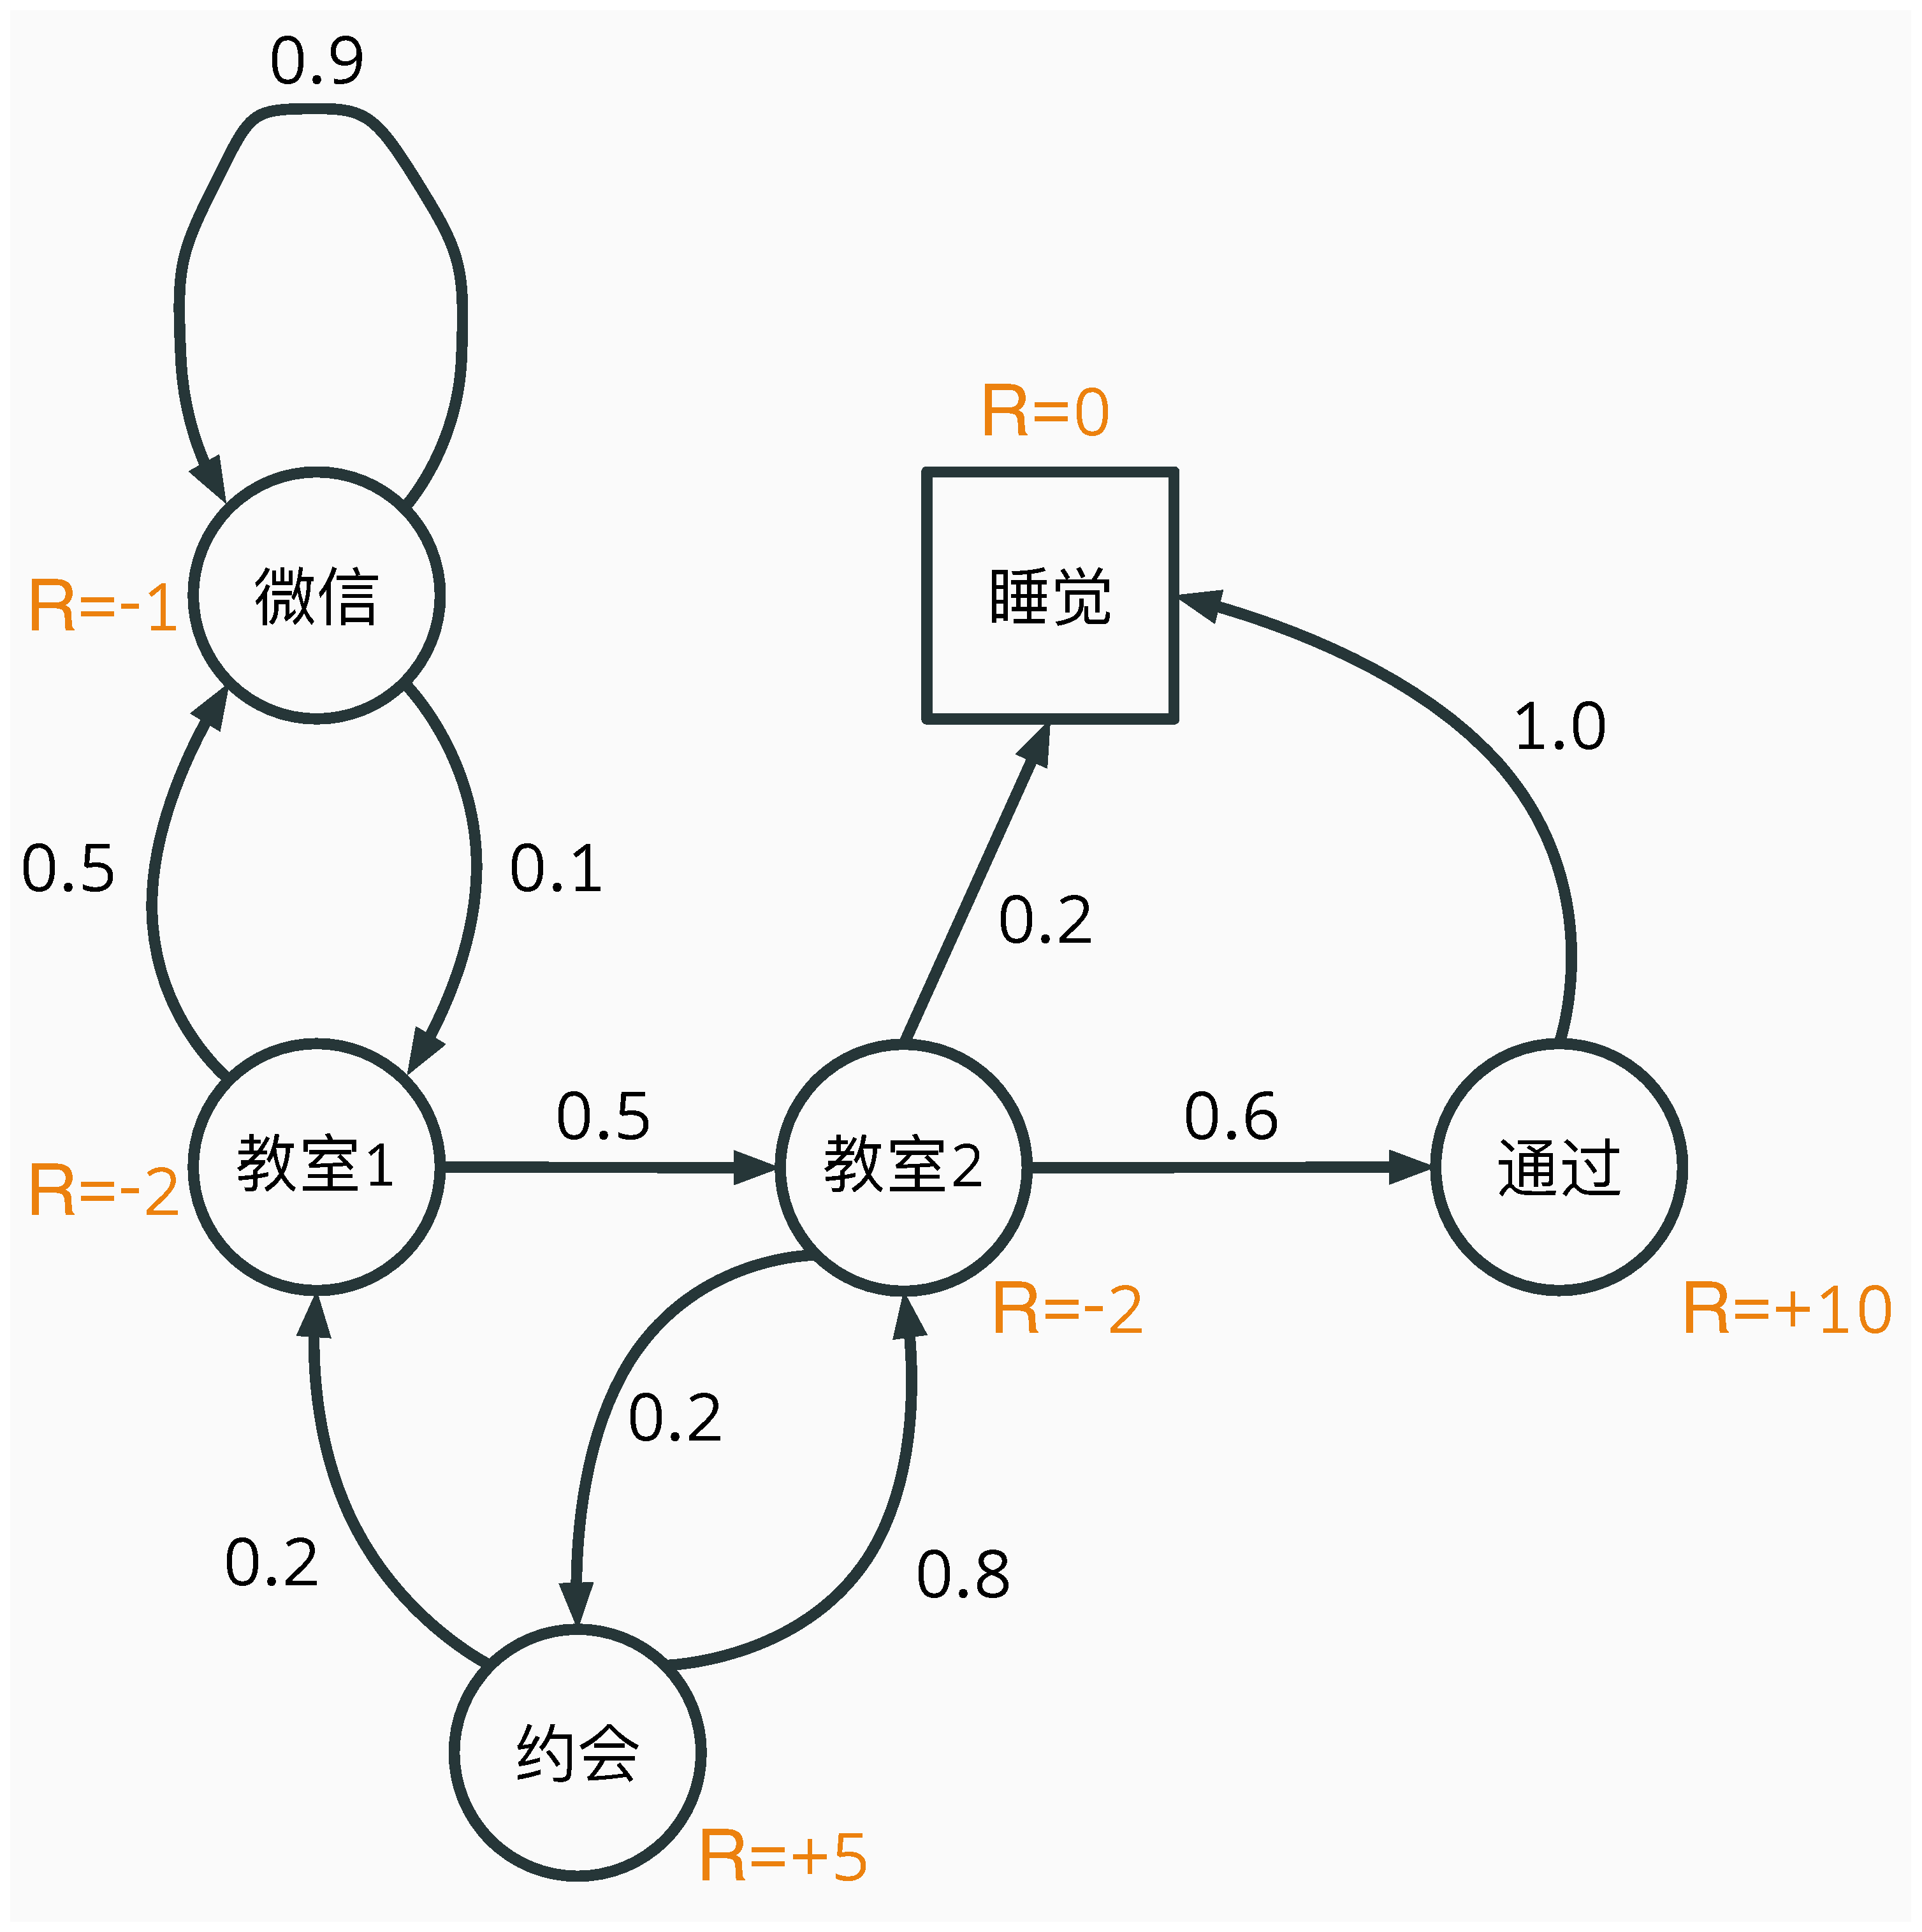
\includegraphics[height=0.8\textheight]{\pref/STR.eps}
\end{figure}


{回报}
\begin{itemize}
    \item MRP中,$t$时刻以后的总\emph{回报}(Return)$G_t$定义为
    \[G_t = R_{t+1}+\gamma R_{t+2} +\dots =\sum_{k=0}^\infty \gamma^kR_{t+k+1}.\]
        \item $\gamma \in[0,1]$衡量了未来下一时段1的奖励在当前时刻的价值.
        \item 未来$k+1$时刻的奖励对当前时刻$t$的作用是$\gamma^k R_{t+k+1}$.
        \item 若$\gamma\to0$,表示对奖励进行“短视”的评估;反之更“远见”.
\end{itemize}


{折扣系数的意义}
\begin{itemize}
    \item 许多MRP和后面学习的MDP都有与时间无关的折扣系数$\gamma <1$,原因:
\begin{itemize}
    \item 起始于对未来不确定性对冲:直接对应于利润率. 
    %具有不确定性,因此未来的回报更有风险,需要一个折扣风险的系数.
    %\item 数学上表示不麻烦.
    \item 动物和人类对即时回报具有偏好.
\end{itemize}
\item 有时也使用非折扣化的MRP(即$\gamma=1$),例如当所有的转移序列都会有固定的终止时间.
\end{itemize}


{价值函数}
\begin{itemize}
    \item 在MRP中,状态\emph{价值函数}(value function)$v(s)$表示从状态$s$出发的期望回报
    \[v(s) = \E(G_t|S_t=s).\]
    \item 价值函数$v(s)$衡量了状态$s$的长期效益.
    \item Markov性:只从当前起考虑未来收益,不考虑历史收益(沉没成本)的影响.
    \item 时齐性:价值函数的定义不依赖于时刻$t$
    (无穷阶段情形).
\end{itemize}



{MRP的Bellman方程}
\begin{itemize}
    \item 价值函数可以被分解为两部分:
\begin{itemize}
    \item 即时回报$\textcolor{red}{R_{t+1}}$
    \item 下一个状态开始的折扣价值 $\textcolor{green}{\gamma v(S_{t+1})}$
\end{itemize}
        \begin{align*}
        v(s) &= \E(G_t|S_t=s) \\
            &= \E(R_{t+1}+ \gamma R_{t+2} + \gamma^2 R_{t+3}+\dots | S_t= s) \\
            &= \E(R_{t+1} + \gamma (R_{t+2}+\gamma R_{t+3}+\dots) | S_t = s) \\
            &= \E(R_{t+1} + \gamma G_{t+1} | S_t = s) \\
            &= \E(\textcolor{red}{R_{t+1}} + \textcolor{green}{\gamma v(S_{t+1})}| S_t=s)\\
            &= {\textcolor{red}{\mathcal R_s} + \textcolor{green}{\gamma \sum_{s'\in \MS}\P_{s,s'}v(s')}}. % HW: 做一下破产博弈的Wald等式. 看一下zfx应随教材1.10三(100页),可以在题目里直接假设停时概率1有限
    \end{align*}
\end{itemize}


{矩阵形式的Bellman方程}
\begin{itemize}
    \item Bellman方程可以用矩阵形式表达:
        \[v = \mathcal R + \gamma \mathcal P v.\]
    这里$v$是列向量$v=(v(s))_{s\in\MS}$.
\end{itemize}


{Bellman方程的解}
\begin{itemize}
    \item Bellman方程是一个线性方程,可以被直接解:
    \[
        v =\mathcal R + \gamma \P v \implies (I-\gamma \P)v = \mathcal R \implies v = (I-\gamma \P)^{-1} \mathcal R.
   \]
    \item 对于$n$个状态的Markov链,计算复杂度为$\O(n^3)$.
    \item 对于较小的MRP可以直接解,太大的MRP开销太大.
    \item 对于大型MRP,可以采用迭代算法,例如:
    \begin{itemize}
        \item 动态规划(dynamic programming)
        \item Monte-Carlo评估(Monte-Carlo evaluation) 
        \item 时序差分学习(temporal-difference learning)
    \end{itemize}
\end{itemize}


\section{Markov决策过程(MDP)}
{Markov决策过程}
\begin{itemize}
    \item \emph{Markov决策过程}(Markov decision process)是一个定义了决策的MRP. 它可以看做一个任意状态都具有Markov性的\emph{环境}.
    \item 一个MDP是五元组$\langle\MS, \textcolor{green}{\mathcal A}, \P, \mathcal R, \gamma\rangle$.
        \begin{itemize}
            \item $\MS$是一个有限的状态集合.
            \item $\textcolor{green}{\mathcal A}$是一个有限的\emph{行动}(action)集合.
            \item $\P$是状态转移概率矩阵,
            \[\P_{ss'}^{\textcolor{green}{a}} = \Pr(S_{t+1} = s' | S_t = s, A_t = \textcolor{green}{a}).\]
            \item $\mathcal R$是一个奖励函数,$\mathcal R_s^{\textcolor{green}{a}} = \E(\textcolor{red}{R_{t+1}} | S_t = s, A_t = \textcolor{green}{a})$,$\textcolor{red}{R_{t+1}}$是进行某一行动到达某一状态后的奖励.
            \item $\gamma$是一个折扣系数$\gamma\in[0,1]$.
        \end{itemize}
    \end{itemize}


{例子:学生MDP}
\begin{figure}
    \centering
    \includegraphics[height=0.8\textheight]{\pref/STD.eps}
\end{figure}


{策略}
\begin{itemize}
    \item     一个\emph{策略}(policy)$\pi$是给定状态下行动的分布,
    \[\pi(a|s) = \Pr(A_t=a | S_t = s).\]
    \item 一个策略完全决定了一个智能体在MDP环境中的行为.
    \item Markov性:MDP的策略取决于当前状态,而非历史状态.
    \item 时齐性:MDP的策略不依赖于时刻$t$.
\end{itemize}


{策略}
\begin{itemize}
    \item 给定一个MDP $\M=\langle\MS,\mathcal A,\P,\mathcal R, \gamma\rangle$和一个策略$\pi$.
    \item $\langle \MS, \P^{\pi}\rangle$是一个Markov链.
    \item $\langle\MS,\P^{\pi}, \mathcal R^{\pi}, \gamma\rangle$是一个MRP.
    \item 其中
\end{itemize}
\[\P_{s,s'}^{\pi} = \E_{a\sim\pi(\cdot|s)}(\P^a_{s,s'})=\sum_{a\in \mathcal A}\pi(a|s)\mathcal P_{s,s'}^{a},\]
    \[\mathcal R_s^{\pi} =\E_{a\sim\pi(\cdot|s)}(\mathcal R^a_s)=\sum_{a\in\mathcal A}\pi(a|s)\mathcal R_s^a.\]


{价值函数}
\begin{itemize}
    \item 在MDP中,状态-价值函数$v_\pi(s)$是从状态$s$出发,遵从策略$\pi$的期望回报
    \[v_\pi(s) = \E_\pi(G_t|S_t=s).\]
    \item     行动-价值函数$q_\pi(s,a)$是从状态$s$出发,采取行动$a$,遵从策略$\pi$的期望回报
    \[q_\pi(s,a) = \E_\pi(G_t|S_t=s,A_t=a).\]
    \item 注意,以上定义都具有Markov性和时齐性.
\end{itemize}


{Bellman期望方程}
\begin{itemize}
    \item 状态-价值函数可以被分解为:即时回报 加 后续状态的折扣价值,
\[v_\pi(s) = \E_\pi(R_{t+1} + \gamma v_\pi(S_{t+1})|S_t=s).\]
\item 行动-价值函数可以被类似地分解,
\[q_\pi(s,a) = \E_\pi(R_{t+1} + \gamma q_\pi(S_{t+1},A_{t+1})|S_t=s,A_t=a).\]
\item 二者之间的关系(全概率公式、一步转移概率):
\[q_\pi(s,a) =\mathcal R_s^a + \gamma \sum_{s'\in \MS}P_{s,s'}^a v_\pi(s').\]
\[v_\pi(s) = \E_{a\sim\pi(\cdot|s)}(q_\pi(s,a))=\sum_{a\in\mathcal A}\pi(a|s)q_\pi(s,a),\]
\end{itemize}


{Bellman期望方程}
\begin{itemize}
    \item 因此,我们得到MDP的Bellman期望方程:
\[v_\pi(s) = \sum_{a\in \mathcal A}\pi(a|s)\left(\mathcal R_s^a + \gamma \sum_{s'\in \MS}\P_{s,s'}^av_\pi(s')\right),\]
\[q_\pi(s,a) = \mathcal R_s^a + \gamma \sum_{s'\in \MS}\P_{s,s'}^a \sum_{a'\in \mathcal A}\pi(a'|s')q_\pi(s',a').\]
\item 矩阵形式:
\[v_\pi = \mathcal R^\pi + \gamma \P^\pi v_\pi = (I-\gamma \mathcal P^\pi)^{-1}\mathcal R^\pi.\]
\end{itemize}


{最优价值函数}
\begin{itemize}
    \item \emph{最优状态-价值函数} $v_\star(s)$ 是所有决策中最大的状态-价值函数
    \[v_\star(s) = \max_\pi v_\pi(s).\]
    \item \emph{最优行动-价值函数} $q_\star(s,a)$是所有决策中最大的行动-价值函数
    \[q_\star(s,a) = \max_\pi q_\pi(s,a).\]
    \item 最优价值函数确定了MDP中的最佳收益.
    \item 解MDP即确定达到最优价值函数的策略.
\end{itemize}


{最优策略}
\begin{itemize}
    \item 然而,每个状态取到最大价值的策略$\pi$可能并不是同一个.
    \item 幸运的是,确实存在一个这样的最优策略. 定义一个策略的偏序:
    \[\pi\ge\pi' \iff \forall s\in\MS\ v_\pi(s) \ge v_{\pi'}(s).\]
\end{itemize}
\begin{theorem}[MDP解的存在性]
对任意MDP,
\begin{itemize}
    \item 存在一个最优策略 $\pi_\star$使得$\forall \pi\ \pi_\star\ge\pi$.
    \item 最优策略取得最优状态-价值函数:$v_{\pi_\star}(s) = v_\star(s)$.
    \item 最优策略取得最优行动-价值函数:$q_{\pi_\star}(s,a)=q_\star(s,a)$.
\end{itemize}
\end{theorem}


{寻找最优决策}
\begin{itemize}
    \item 可以通过最大化$q_\star(s,a)$来寻找:
    \begin{itemize}
        \item 固定$s$.
        \item 找到一个$a_\star$使得$q_\star(s,a_\star)=\max_{a}q_\star(s,a)$,令$\pi_\star(a_\star|s)=1$.
        \item 对$\forall a\neq a_\star$,$\pi_\star(a|s)=0$.
    \end{itemize}
    \item 证明:根据选法,$\pi_\star$取得最优行动-价值函数.
    \item 由$v_\pi(s) = \E_{a\sim\pi(\cdot|s)}(q_\pi(s,a))\leq \E_{a\sim\pi(\cdot|s)}(q_\star(s,a))\leq q_\star(s,a_\star)=v_{\pi_\star}(s)$知$\pi_\star$取得最优状态-价值函数.
    \item 推论:对任意MDP,总存在一个非随机的最优决策.
    \item 如果我们知道$q_\star(s,a)$,我们就能获得最优决策. % HW: 找一个简单一点的例子,让他们算一下最优策略
\end{itemize}


{Bellman最优性方程}
\begin{itemize}
    \item 最优价值函数由Bellman最优性方程联系:
\[v_\star(s) = \max_a q_\star(s,a),\]
\[q_\star(s,a) = \mathcal R_s^a + \gamma \sum_{s'\in \MS}\P_{s,s'}^av_\star(s'),\]
\[v_\star(s) = \max_a\left\{\mathcal R_s^a + \gamma \sum_{s'\in \MS}\P_{s,s'}^av_\star(s')\right\},\]
\[q_\star(s,a) = \mathcal R_s^a+\gamma \sum_{s'\in \MS}\P_{s,s'}^a\max_{a'}q_\star(s',a').\]
\end{itemize}


{解Bellman最优性方程}
    \begin{itemize}
        \item Bellman最优性方程不是线性的. 因此没有解析形式的(closed form)解.
        \item 但是MDP的数值解是可以多项式时间求出来的.
        \item 我们一般采用迭代算法求解:
        \begin{itemize}
            \item 价值迭代(value iteration)
            \item 策略迭代(policy iteration)
            \item Q-learning
            \item Sarsa
        \end{itemize}
    \end{itemize}

{关于Bellman方程}
\begin{itemize}
    \item Bellman方程是强化学习(reinforcement learning)、经济学动态优化(dynamic optimization)的核心.
    \item Bellman方程的推导是Markov链中最为常用的技巧:考虑从当前状态转移到下一状态,利用全概率公式,一步转移会将两个状态之间的概率(期望)用递推公式联系起来.
    \begin{itemize}
        \item 随机过程中的例子:前向方程、Wald等式、调和函数(harmonic function).
        \item 后面的HMM也是类似的例子.
    \end{itemize}
\end{itemize}


\section{隐Markov模型(HMM)}

问题的引入

\begin{itemize}
    \item 我们考虑Markov链上的另一种应用.
    \item 在统计学和机器学习中,我们有时候要处理一类含时间的数据.
    \item 最简单的情况是回归,即数据完全由所处时刻决定.
    \item 但是通常,现在的数据依赖于过去的数据.
    \item 因此,一种最简单的考虑就是数据依赖于Markov链,这就是隐Markov模型.
\end{itemize}


{隐Markov模型}
\begin{itemize}
    \item 一个\emph{隐Markov模型}(hidden Markov model,HMM)是一列随机变量$X_1,X_2,\dots, X_t$,满足:
    \begin{itemize}
        \item $X_t$的分布仅依赖于隐状态$Z_t$,即$\Pr(X_1,\dots,X_t|Z_1,Z_2,\dots,Z_t)=\prod_i \Pr(X_i|Z_i)$.
        \item $\{Z_t\}$构成一条Markov链.
    \end{itemize}
\end{itemize}
\begin{figure}
    \centering
    \includegraphics[width=0.6\textwidth]{\pref/HMM.eps}
\end{figure}


{有限观测HMM}
\begin{itemize}
    \item 一个HMM包含:
    \begin{itemize}
        \item $\mathcal Z$
        : 有限的状态集合.
        \item $\mathcal X$: 有限的观测集合.
        \item $T: \mathcal Z\times\mathcal Z\to \R_{\geq 0}$,$\mathcal Z$的转移概率.
        \item $M:\mathcal Z\times \mathcal X\to \R_{\geq 0}$,给定状态时的观测概率(条件概率).
        \item $\lambda:\mathcal Z\to\R_{\geq 0}$,初始状态的先验概率分布列.
    \end{itemize}
    \item 如果随机过程$\{X_t\}$的值域是有限集,我们则可以用矩阵表达HMM.
    \begin{itemize}
    \item $T$是$\{Z_t\}$的转移矩阵.
    \item $M$是观测矩阵:$M_{i,k} = \Pr(X_t=k|Z_t=i)$.
    \item $\lambda$是一个概率向量.
    \end{itemize}
\end{itemize}


\subsection{评估问题}
{HMM的评估}
\begin{itemize}
   \item 给定一个特定的HMM,它对实际观测序列的拟合程度有多好?
   \item 记号:随机向量$X=(X_1,\dots,X_t)$,$Z=(Z_1,\dots,Z_t)$.
   \item  HMM的\emph{评估}(evaluation)问题:给定一个HMM $\M$,以及它的观测历史$x=(x_1,x_2,\dots,x_t)$,计算$\Pr(X=x|\M)$.
   \item 关键困难:我们不知道状态历史$Z=(z_1,z_2,\dots,z_t)$.
\end{itemize}


{朴素方法}
    \begin{itemize}
    \item 直接使用条件概 率进行推导:
    \[
        \Pr(X=x|\M) =\sum_{Z=(z_1, \dots, z_t) \in \mathcal Z} \Pr(X=x|Z=z, \M)\Pr(Z=z|\M),
    \]
    \[
        \Pr(X=x|Z=z,\M) = \prod_{i=1}^t \Pr(X_i = x_i| Z_i = z_i) = M_{z_1,x_1}\cdot M_{z_2,x_2}\dots M_{z_t,x_t},
    \]
    \begin{align*}
        \Pr(Z=z|\M) &= \Pr(Z_1 = z_1) \prod_{i=2}^t\Pr(Z_i = z_i| Z_{i-1} = z_{i-1}) 
        \\
        &= \lambda_{z_1}\cdot T_{z_1,z_2}\cdot T_{z_2,z_3}\dots T_{z_{t-1},z_t}.
    \end{align*}
    \item 时间复杂度: $\O(t|\mathcal Z|^t)$.
    \end{itemize}


{前向算法}
    \begin{itemize}
    \item 思路:类似前向方程,我们可以从前$k$步的结果推出前$k+1$步的结果. 因此可以列出递推方程.
    \item 记号:$X_{i:j}=(X_i,\dots,X_j)$.
    \item 具体地,定义$\alpha_k(z):= \Pr(X_{1:k}=x_{1:k}, Z_k=z| \M)$,我们有
    \begin{itemize}
        \item $\alpha_1(z) = \lambda(z)M_{z,x_1}$.
        \item $\alpha_{k+1}(z) = \sum_{z' \in \mathcal Z}\alpha_{k}(z')T_{z',z}M_{z,x_{k+1}}$.
    \end{itemize}
    \item $\Pr(X=x| \M) = \sum_{z\in \mathcal Z}\alpha_t(z)$.
    \item 时间复杂度 $\mathcal O(t|\mathcal Z|^2)$.
\end{itemize}



{后向算法}
   \begin{itemize}
    \item 类似后向方程,从前$k+1$步的结果推出前$k$步的结果. 同样可以列出递推方程.
    \item 定义$\beta_k(z):=\Pr(X_{k+1:t}=x_{k+1:t} | Z_k=z,\M)$,我们有
    \begin{itemize}
        \item 当$k = t$,$\beta_k(z) = 1$.
        \item 当$1 \le k < t$,$\beta_{k}(z) = \sum_{z' \in \mathcal Z}T_{z,z'}M_{z',x_{k+1}}\beta_{k+1}(z')$.
    \end{itemize}
    \item $\Pr(X=x| \M) = \sum_{z\in \mathcal Z}\lambda(z)M_{z,x_1}\beta_1(z)$.
    \item 时间复杂度 $O(t|\mathcal Z|^2)$.
\end{itemize}


\subsection{解释问题}
{HMM的解释问题}
    \begin{itemize}
    \item HMM的\emph{解释}(explanation)问题:给定一个 HMM $\M = (\mathcal Z, \mathcal X, T, M, \lambda)$, 一列观测历史$x = (x_1, x_2, \dots, x_t)$, 寻找一个状态序列,能最好地解释这些历史观察.
    \item 具体地,我们考虑如下四个问题
    \begin{enumerate}
        \item 过滤(filtering):计算$\Pr(Z_k = s|X_{1:k}=x_{1:k}, \M)$.
        \item 平滑(smoothing): 计算$\Pr(Z_k = s|X=x, \M)$,$k < t$.
        \item 预测(prediction): 计算$\Pr(Z_k = s|X=x, \M)$,$k > t$.
        \item 解码(decoding): 找到最有可能的状态序列 $z = (z_1, z_2, \dots, z_t)$.
    \end{enumerate}
\end{itemize}




{过滤:$\Pr(Z_k = s|X_{1:k}=x_{1:k}, \M)$}
\begin{itemize}
    \item 回顾:$\alpha_k(s)= \Pr(X_{1:k}=x_{1:k}, Z_k=s| \M)$. 
    \item 我们有
    \begin{align*}
        \Pr(Z_k = s|X_{1:k}=x_{1:k}, \M) & = \frac{\Pr(X_{1:k}=x_{1:k}, Z_k=s| \M)}{\Pr(X_{1:k}=x_{1:k}| \M)} \\
        &= \frac{\alpha_k(s)}{\sum_{z\in\mathcal Z}\alpha_k(z)}.
    \end{align*}
\end{itemize}


{平滑:$\Pr(Z_k = s|X=x, \M)$,$k < t$} 
\begin{itemize}
    \item 回顾:$\alpha_k(s)= \Pr(X_{1:k}=x_{1:k}, Z_k=s| \M)$.
    \item 回顾:$\beta_k(s)=\Pr(X_{k+1:t}=x_{k+1:t} |Z_k=s, \M)$.
    \item 可以证明:
        \[\Pr(z_k = s|X=x, \M)=\frac{\beta_k(s)\alpha_k(s)}{\sum_{z\in\mathcal Z}\alpha_t(z)}.
    \]% HW: 推导这个
    % \[\Pr(X_k = s|z, \M) =& \frac{\Pr(z_{1:k}, z_{k+1:t}, X_k=s| \M)}{\Pr(z| \M)} 
    %     \\
    %     =& \frac{\Pr(z_{k+1:t}| z_{1:k}, X_k=s,\M)\Pr(z_{1:k}, X_k=s| \M)}{\Pr(z| \M)}
    %     \\
    %     =& \frac{\Pr(z_{k+1:t}| X_k=s,\M)\Pr(z_{1:k}, X_k=s| \M)}{\Pr(z| \M)}
    %     \\
    %     =& \frac{\beta_k(s)\alpha_k(s)}{\Pr(z| \M)} = \frac{\beta_k(s)\alpha_k(s)}{\sum_{x\in\mathcal X}\alpha_t(x)} 
    % \]
\end{itemize}



{预测:$\Pr(Z_k = s|X=x, \M)$,$k > t$.}
\begin{itemize}
    \item 首先用过滤计算 $\lambda=\Pr(Z_t = s|X=x, \M)$.
    \item 然后用 $\lambda$ 作为Markov的初始状态,向前计算$k-t$步.
\end{itemize}


{*解码:Viterbi算法}
\begin{itemize}
    \item 定义 
    $$\delta_k(s) = \max_{Z_{1:k-1}}\Pr(Z_{1:k} = (z_{1:k-1}, s), X_{1:k}=x_{1:k}| \M).$$
    \item 根据一步转移,我们有
    $$\delta_{k+1}(s) = \max_{q\in \mathcal Z}\{\delta_k(q)T_{q,s}\}M_{s,x_{k+1}}.$$
    \item 问题转化为: 记录最高概率的路径,这是一个动态规划问题.
\end{itemize}


\newcommand{\pre}{\mathrm{Pre}}
{*解码: Viterbi算法}
\begin{itemize}
    \item 初始化:
    \begin{itemize}
        \item $\delta_1(s) = \lambda(s)M_{s,z_1}$.
        \item $\pre_1(s) = \varnothing$.
    \end{itemize}
    \item 对 $k=1, 2, \dots, t-1$,$s \in \mathcal Z$:
    \begin{itemize}
        \item $\delta_{k+1}(s) = \max_{q\in \mathcal Z}\{\delta_k(q)T_{q,s}\}M_{s,x_{k+1}}$.
        \item $\pre_{k+1}(s) = \argmax_{q\in \mathcal Z}\{\delta_k(q)T_{q,s}\}$.
    \end{itemize}
    \item $z_t = \argmax_{s \in \mathcal Z}\delta_{t}(s)$.
    \item 对 $1 \le k < t$,$z_k = \pre_{k+1}(z_{k+1})$.
    \item 时间复杂度: $\mathcal O(t|\mathcal Z|^2)$.
\end{itemize}

\endgroup

\part{信息与数据}\label{part:information-data}
\chapter{不动点理论}\label{chap:fixed-point-theory}
\chapter{不动点理论}\label{chap:fixed-point-theory}
\chapter{不动点理论}\label{chap:fixed-point-theory}

\part{决策与优化}\label{part:decision-optimization}
\chapter{凸分析}\label{chap:convex-analysis}

本章将会建立关于决策与优化的基本理论,这些方法论都是数据驱动的机器学习的基础,他们涉及从数据到建立模型的步骤(即训练). 优化与分析有着密不可分的联系,所以本章我们会立足优化问题的一些基本事实,建立凸分析理论. 凸分析是优化理论的基础.

\section{决策与优化的基本原理}
\subsection{统计决策理论}\index{统计决策理论}
\lhysays{这部分要细化}

我们在前一部分讨论过,数据(或者说信息)的意义总是体现在集合的对象中,我们把我们所关心的集合对象称为(随机)\emph{总体}\index{总体} $P$. 从概率论角度看,总体就是一个概率分布. 现在我们从总体$P$中抽取一个\emph{样本}\index{样本} $X$. 这件事情在概率论上意味着我们得到了一个随机变量$X$服从分布$P$. 拿到样本之后,我们的任务是做出\emph{好的决策},因此,决策$T$是一个依赖$X$的函数. 比如说,$P$是所有大学生的身高,$X$是随机抽选一个人测量的身高,我们的决策$T$是估计大学生的平均身高. 

“好的决策”指的是函数$T$能够具备某些量化指标. 其中非常常用的一个方法是通过\emph{损失函数}\index{损失函数}来衡量,它是总体$P$和决策$T(X)$的函数,即$L(P,T(X))$. 损失函数在不同语境下有不同称呼. \emph{损失函数}是机器学习和数理统计语境下常用的称呼. 在控制理论中以及机器学习中,它被称为\emph{代价函数}\index{代价函数}. 在经济学和金融学的风险理论中,损失函数被称为\emph{风险函数}\index{风险函数},它意味着个体在面对不确定的环境下所需要面对的风险. 而在优化理论中,损失函数往往被称为\emph{目标函数}\index{目标函数},表明所要优化的对象. 

决策$T$的一种量化指标是最小化期望意义下的损失函数:
    \[\min_{T}\E_{X\sim P}(L(P,T(X))).\]
在经济学中,这一量化指标实际上是von Neumann和Morgenstern \emph{期望效用理论}\index{期望效用理论}的具体体现. 这一理论认为,个体在面对不确定的环境时,会选择最大化期望效用的决策;在风险理论的语境下,则是最小化期望风险的的决策. 

现在我们考虑一个非常一般的决策任务. 假设我们的任务是估计函数$f$,但是我们只知道观测到的自变量$X$(来自总体$P$)以及它的函数值$Y=f(X)$,我们的决策是函数的估计值$\hat f$. 在机器学习中,$f$通常是需要训练的模型. 我们可以写出若干种损失函数:
\begin{itemize}
    \item 平方($L^2$)损失函数\index{损失函数!平方~}\index{损失函数!$L^2$~}:$L(P,T(X))=(Y-\hat f(X))^2$. 使用此损失函数的时候,我们要假定$f$在实数范围取值. 
    \item $L^1$损失函数\index{损失函数!$L^1$~}:$L(P,T(X))=|Y-\hat f(X)|$. 使用此损失函数的时候,我们要假定$f$在实数范围取值. 
    \item SVM损失函数(hinge损失函数)\index{损失函数!SVM~}\index{损失函数!hinge~}:$L(P,T(X))=\max\{0,1-Y\cdot\hat f(X)\}$. 使用此损失函数的时候,我们一般要假定$f(X)\in[-1,1]$. 
    \item 交叉熵损失函数\index{损失函数!交叉熵~}:$L(P,T(X))=CH(\hat f(X),Y)$.
\end{itemize}

这些损失函数会用在不同的场景之中. 通常来说,机器学习中有两类问题:\emph{回归问题}\index{回归问题}和\emph{分类问题}\index{分类问题}和. 他们两个的区别主要在于回归问题中$f$取值为实数,而且通常随自变量连续变化;而分类问题中$f$只取有限多个值,他们通常被作为标签(比如这张图片是人还是青蛙)使用. 在回归问题中,我们通常使用平方损失函数或者$L^1$损失函数;在分类问题中,我们通常使用SVM损失函数或者交叉熵损失函数. 

\subsection{优化问题}\index{优化问题}
现在我们从决策过渡到优化. 在最简单的决策问题中,我们的目标就是找到某个$x$使得(期望)损失函数$f$最小. 此时,问题的一般形式为:
\begin{alignat*}{2}
\min_{x}&\quad f(x)\\
\text{s.t.}&\quad f_i(x)=0,&\quad i=1,\dots,m,\\
&\quad g_j(x)\leq 0,&\quad j=1,\dots,n,\\
&\quad x\in\Omega.
\end{alignat*}
这里,s.t(subject to)之后的内容表明了$x$取值的限制,因此被称为\emph{约束}\index{约束}. 其中$f_i(x)=0$和$g_j(x)\leq 0$被称为\emph{函数约束}\index{约束!函数~},而$x\in\Omega$被称为\emph{集合约束}\index{约束!集合~}.

优化的基本任务就是找到$x$最小化损失函数. 

根据损失函数$f$、约束条件$f_i$和$g_j$的不同性质,我们可以对优化问题进行分类:
\begin{itemize}
\item 无约束优化\index{优化问题!无约束优化}:约束条件$f_i$和$g_j$实际上不存在,即$m=n=0$,并且$\Omega$是全空间,比如$\R^n$.
\item 有约束优化\index{优化问题!有约束优化}:至少存在一个约束条件,即$\min\{m,n\}\geq 1$,或者$\Omega$不是全空间. 
\item 光滑优化\index{优化问题!光滑优化}:损失函数和约束条件都是可微函数.\footnote{光滑这一词的含义在不同的文献中大相径庭,它可以指(连续)可微、连续可微、二次(连续)可微或者无穷次可微. }
\item 线性优化\index{优化问题!线性优化}:损失函数和约束条件都是线性函数(形如$a^\t x+b$).
\end{itemize}

\begin{remark}
    \lhysays{介绍一下控制理论与优化理论的异同,特别是连续控制和随机优化. }
\end{remark}

下面我们看几个经典的优化例子. 
\begin{example}[最小二乘法]\label{ex:least-square}\index{最小二乘法}
    给定矩阵$A\in\R^{m\times n}$和向量$b\in\R^m$,考虑如下优化问题:
    \begin{alignat*}{2}
    \min_{x}&\quad \norm{Ax-b}_2^2\\
    \text{s.t.}&\quad x\in\R^n.
    \end{alignat*}
    这个问题被称为\textbf{最小二乘法}\index{最小二乘法}. 目标函数可以被写为$(Ax-b)^\t(Ax-b)$,因此最小二乘法是一种典型的无约束光滑优化问题. 

    最小二乘法的解$x^*$实际上是\emph{投影}\index{投影}解:$b$的行向量投影到$A$的列向量形成的线性空间,正好是$Ax^*$. \lhysays{加个图,补全细节} 因此,求投影也可以被写作一个优化问题.
\end{example}

\begin{example}[线性规划]\label{ex:linear-programming}\index{线性规划}
    给定矩阵$A\in\R^{m\times n}$和向量$b\in\R^m$,考虑如下优化问题:
    \begin{alignat*}{2}
    \min_{x}&\quad c^\t x\\
    \text{s.t.}&\quad Ax\leq b,\\
    &\quad x\geq 0.
    \end{alignat*}
    这个问题被称为\textbf{线性规划}\index{线性规划}. 目标函数和约束条件都是线性的,因此线性规划是一种典型的线性优化问题. \lhysays{加个图,补全细节}
\end{example}

上面两个例子远远不能覆盖所有的优化问题,实际上,相当多的运筹学、机器学习和计算机科学中的问题都可以被视作(非线性)优化问题. 
\begin{itemize}
    \item 运筹学:线性规划、二次规划、整数规划、网络流问题、组合优化问题等.
    \item 金融学:投资组合优化、风险控制等.
    \item 机器学习:模型的训练.
    \item 计算机科学:图论中的极值问题,例如最短路径问题、最小生成树问题等.
\end{itemize}
因此,如果有一个能够解决通用优化问题的灵丹妙药,那么将会有极其重大的意义. 然而我们后面将会看到,一般的优化是一个难解的问题,更严谨一点说,不存在通用高效算法. 

我们先需要明确解优化问题的算法到底是什么. 我们通过给出算法的一些特征来最终明确这一点. 大部分优化算法都用了\textbf{迭代法}\index{迭代法}的思想:算法$A$接受一个自变量$x$,输出一个自变量$A(x)$,并把它作为下一轮的输入. 此外,一个算法还应该具有\textbf{通用性}\index{通用性},即它必须要能解决一类优化问题$F$. 然后,算法具备通用性就意味着它在进行\textbf{黑箱优化}\index{黑箱优化}:$F$必须要给算法提供必要的信息来完成求解,我们将这样的提供机制抽象为\textbf{先知}\index{先知},记为$\O$. 具体来说算法输入$x$给$\O$,$\O$返回一些信息给算法(例如$x$处的函数值、导数值、Hessian矩阵).

接下来的问题是衡量优化算法的性能好坏. 我们关注的是\emph{最坏情况},也就是说假如我们关注的是问题类$P\subseteq F$,那么,我们要看的是优化算法在$P$中最差的表现如何. 衡量优化算法性能的指标有以下几个:

\begin{itemize}
    \item \emph{近似程度}\index{近似程度}:我们需要求在允许误差$\epsilon$的情况下的近似解. 例如,函数值不大于最优值的$\epsilon$,或者离最优点距离不超过$\epsilon$. 考虑近似解是优化问题非常重要的一个想法,因为计算机的表示精度是有限的,我们不可能在所有情况下都求出精确解,所以求近似解是合理的要求. 
    \item \emph{运行时间}\index{运行时间}(\emph{收敛速度}\index{收敛速度},\emph{复杂度}\index{复杂度}):找到目标近似解需要调用先知的次数. 通常来说,运行时间会随近似度要求变高而变长,因此运行时间是一个关于近似程度的函数.
\end{itemize}

\begin{remark}
    通常来说,优化算法的执行过程中还会进行除了调用先知之外的操作,例如进行加减乘除. 然而,如果我们把所有这些操作都算入复杂度之中,算法的分析会变得非常困难,因此我们通常只考虑调用先知的次数. 这样做的合理性在于,每一次的加减乘除等额外操作,几乎都是因为调用一次先知所以才进行的,因此我们可以把这些额外操作的时间都算入先知调用的时间之中. 
\end{remark}

有了上面这些准备,我们就可以将“没有万能算法”这一陈述写成定理了. 

\begin{theorem}[没有免费午餐定理]\label{thm:no-free-lunch}\index{没有免费午餐定理}\lhysays{给一个证明,以及更加严格的表述}
    设$F$是有限个优化问题的集合,$F$上有一个任意的概率分布. 考虑一个$F$上的优化算法,记号$d_t$表示$t$轮迭代之后算法产生的点列
    \[(x_t(1),y_t(1)),\dots,(x_t(t),y_t(t)).\]
    给定迭代轮数$t$,优化问题$f$,算法$A$,优化过程所产生的点列概率分布为$P(d_t|f,t,A)$. 那么,对任意优化算法$A_1,A_2$,
    \[\sum_{f\in F} P(d_t|f,t,A_1)=\sum_{f\in F} P(d_t|f,t,A_2).\]
\end{theorem}
这一定理意味着,对特定的点列,任何算法在所有实例上产生它的概率总和是一样的. 

那么,点列和“没有万能算法”有什么样的关系呢?实际上,衡量算法性能的指标和点列有非常密切的联系. 比如说,算法花了$k$步找到一个$\epsilon$-近似解,用点列的语言来说就是算法迭代产生的点列,长度至多是$k$并且最后一个点距离最优解距离不大于$\epsilon$. 粗略地说,任意点列成立的性质意味着任意指标成立的性质. 因此,对于任何一类优化问题来说,不论以何种指标来衡量性能,优化算法在某些问题上表现出来的突出性能一定会在另一些问题上被抵消. 没有一个万能的算法可以高效解决所有优化问题!


\subsection{例子:网格搜索算法}

前面对于概念的讨论依然非常抽象,所以下面我们看一个具体的例子,这个例子将会展示从算法分析的角度,优化所关注的主要问题. 考虑如下优化问题:
\begin{equation}
    \begin{aligned}
    \min_{x}&\quad f(x)\\
    \text{s.t.}&\quad x\in[0,1]^n.
\end{aligned}\label{opt:gird-search}
\end{equation}
其中$f(x)$是Lipschitz连续函数,即它满足
    \[|f(x)-f(y)|\leq L\norm{x-y}_\infty,\quad\forall x,y\in[0,1]^n.\]
关于优化算法的假设如下. 首先,我们可以访问\textbf{零阶先知}\index{先知!零阶~},即$\O(x)=f(x)$. 其次,优化算法需要去找到\textbf{$\epsilon$-近似解},即函数值至多比最小值大$\epsilon$的解.

\begin{remark}
\index{先知!零阶~}\index{先知!一阶~}
        在优化中,我们会经常使用词语“零阶”“一阶”等等,所谓的“阶”指的是函数导数阶数,零阶先知指的是我们可以访问函数值,一阶先知指的是我们可以访问一阶导数,以此类推. 后面还会有零阶条件、一阶条件等等,他们的含义类似. 
\end{remark}

我们考虑一个非常简单的算法,他被称为\emph{网格搜索}\index{网格搜索}:
\begin{itemize}
    \item 将$[0,1]$等分成$p$份,$[0,1]=[0,1/p]\cup\dots[(p-1)/p,1]$.
    \item 遍历$(p+1)^n$个格点:
    \[x_{(i_1,\dots,i_n)}=\left(\frac{i_1}{p},\dots,\frac{i_n}{p}\right)^\t,\]
    $i_k\in\{0,1,\dots,p\}$.
    \item 对每个格点询问先知得到其函数值,输出函数值最小的一个(记为$(\bar{x},f(\bar x))$).
\end{itemize}

我们对于网格搜索算法问的问题是,它的复杂度如何. 也就是说,它需要调用先知多少次才能找到一个$\epsilon$-近似解?我们从一个引理开始. 

\begin{lemma}\label{lemma:gird-search}
    设 \eqref{opt:gird-search} 的最优值为$f^*$,那么
\[f(\bar x)-f^*\leq\frac{L}{2p}.\]
\end{lemma}
\begin{proof}
设$x^*$是最优点,存在一个方格包含$x^*$:
\[x_{(i_1,\dots,i_n)}\leq x^*\leq x_{(i_1+1,\dots,i_n+1)}.\]
这个方格的长为$1/p$,所以我们可以选取方格的某个顶点$\hat x$,使得它的每一个轴离$x^*$的距离都不超过$1/(2p)$.\lhysays{画个图}

于是根据Lipschitz条件,
    \[f(\bar x)-f^*\leq f(\hat x)-f(x^*)\leq L\norm{\hat x- x^*}_\infty\leq \frac{L}{2p}.\]
\end{proof}

利用这个引理,我们可以证明网格搜索算法的复杂度.
\begin{theorem}
    网格搜索算法可以找到找到一个$\epsilon$-近似解,其调用$\O$的次数至多为
    \[\left(\left\lfloor\frac{L}{2\epsilon}\right\rfloor+2\right)^n.\]
\end{theorem}
\begin{itemize}
    \item 证明:取$p=\lfloor L/(2\epsilon)\rfloor+1$,代入\Cref{lemma:gird-search} 即可.
\end{itemize}

 网格搜索法的运行时间给了优化问题 \eqref{opt:gird-search} 一个求解时间的\textbf{上界}. 然而这个上界维数呈指数关系,通常来说都是不可接受的复杂度. \eqref{opt:gird-search} 会有更好的算法呢? 这就是\textbf{下界问题}\index{下界问题}. 令人惊讶的是,对于这一个问题,我们可以证明网格搜索法是渐近意义下最优的!

\begin{theorem}\label{thm:gird-search-lower-bound}
    设$\epsilon<L/2$,任何访问$\O$的算法(零阶算法)找到 \eqref{opt:gird-search} 的 $\epsilon$-近似解至少需要调用$\O$
    \[\left\lfloor\frac{L}{2\epsilon}\right\rfloor^n\]
    次.\lhysays{改一下表述,看不懂}
\end{theorem}
\begin{proof}
设$p=\lfloor L/(2\epsilon)\rfloor$,对任意算法$A$,我们尝试构造一个函数,使得$A$调用$\O$ $p^n$次时最多找到一个$\epsilon$-近似解.

构造思路:对任何测试点,使得$\O$总是返回$0$,于是,算法$A$只能找到$f=0$的解$\bar{x}$. 注意到算法只能根据先知的返回来进行操作,因此我们先假定这样的函数存在. \lhysays{改一下,读不懂}. 

根据鸽巢原理,网格中至少有一个长为$1/p$的小方格$B$内部没有包含任何测试点. 假设这个小方格的中心是$x^*$,构造$\bar f(x)=\min\{0,L\norm{x-x^*}_\infty-\epsilon\}$. 容易看出,$\bar f$是$L$-Lipschitz函数,并且最小值为$-\epsilon$.

函数$\bar f$非零的点只在方格$B'=\{x\in[0,1]^n:\norm{x-x^*}_\infty\leq\epsilon/L\}$内部. 因为$1/(2p)\geq \epsilon/L$,所以$B'\subseteq B$. 所以所有测试点上$\O$都会返回$0$,这是一个$\epsilon$-近似解. 因此$A$通过小于$p^n$次对$\O$的调用最多只能找到$\epsilon$-近似解.
\end{proof}

以上两个结论分别给出了 \eqref{opt:gird-search} 问题的上下界,对比他们:
\begin{center}
\begin{minipage}[t]{0.4\textwidth}
问题的上界:
\[\left(\left\lfloor\frac{L}{2\epsilon}\right\rfloor+2\right)^n\]
\end{minipage}
\begin{minipage}[t]{0.4\textwidth}
问题的下界:
    \[\left\lfloor\frac{L}{2\epsilon}\right\rfloor^n\]
\end{minipage}
\end{center}
尽管网格搜索是一个很慢的算法,但是我们证明了,在渐近意义下,优化问题 \eqref{opt:gird-search} 的最优算法就是网格搜索!因此,我们可以说,一般的优化问题是难解的. 

当我们聚焦在特定的问题类上,优化问题并不一定是难解的. 比如,线性规划可以在关于约束个数和变量个数的多项式时间内解出精确解. 然而,现实中大部分重要的问题并不是线性的,因此,我们接下来的关键问题是\textit{识别出一类可以快速求解的非线性优化问题},这就是凸函数的意义. 


\section{凸函数}\label{sec:convex-function}\index{凸函数}

我们首先看无约束优化,看看什么样的损失函数可以快速求最小值. \textbf{梯度下降方法}\index{梯度下降方法}是最古老也最常用的方法. 梯度下降每步计算函数的导数(梯度),然后朝着负梯度方向移动到下一个点. 与梯度下降算法相关的最小值必要条件是\emph{一阶条件}\index{一阶条件}. 

\begin{theorem}[一阶条件]
    如果$x^*$是可微函数$f$的局部最小值,那么
    \[f'(x^*)=0.\]
\end{theorem}

\begin{proof}
根据局部最小值的定义,存在$r>0$,对于任意$\norm{y-x^*}<r$,$f(y)\geq f(x^*)$. 因此$f(y)=f(x^*)+\inner{f'(x^*)}{y-x^*}+o(\norm{y-x^*})\geq f(x^*)$. 因此,对任意$s\in\R^n$,$\inner{f'(x^*)}{s}\geq 0$. 考虑方向$s$和$-s$可得$\inner{f'(x^*)}{s}=0$. 由$s$的任意性,$f'(x^*)=0$.
\end{proof}

\renewcommand{\F}{\mathcal{F}}

现在,从一阶条件出发,我们考虑如下优化函数类$\F$,满足如下三个假设:
\begin{itemize}
    \item 假设1:对任意$f\in\F$,如果$x$满足一阶条件,那么$x$是$f$的全局最小值点.
    \item 假设2:对任意$f,g\in\F$,$\alpha,\beta\geq 0$,$\alpha f+\beta g\in\F$.
    \item 假设3:线性函数$f(x)=\inner{\alpha}{x}+b\in\F$.
\end{itemize}
假设1使得利用一阶条件的算法可以找到全局最优解. 假设2描述了对$\F$封闭的操作,这样的操作实际上就是要求函数对线性组合封闭. 要求系数$\alpha$和$\beta$非负是为了保证一阶条件得到的确实是最小值而不是最大值. 一个例子是,如果$x^2\in\F$,并且线性组合不限制非负系数,那么$-x^2\in\F$,但是后者一阶条件对应的是最大值而非最小值,这就会与假设1矛盾.  假设3提供了$\F$的基本函数,即线性函数. 我们之前说过,线性规划是易解的,所以$\F$至少要包含线性函数. 

从这三个假设出发,我们可以给出函数类$\F$的刻画. 

固定一个函数$f\in\F$,一个点$x\in\R^n$,定义$\phi(y)=f(y)-\inner{f'(x)}{y}$. 根据假设2和假设3,$\phi(y)\in\F$. $\phi'(y)|_{y=x}=f'(x)-f'(x)=0$,根据假设1,$x$是$\phi$的全局最小值. 因此,$\phi(y)\geq\phi(x)$,即
\begin{equation}
    f(y)\geq f(x)+\inner{f'(x)}{y-x}.\label{eq:def-convex}
\end{equation}
这一不等式给出了\textbf{可微凸函数}\index{凸函数}的定义:任意$x,y$都满足 \eqref{eq:def-convex} 的函数. 这一不等式有很强的几何直观,从$x$处做函数$f$的切线,那么切线上的点都在函数下方. 从这个角度来看,凸函数的定义是向下凸的函数. \lhysays{画个图}

非常有趣的是,$\F$完全由可微凸函数组成,这一点可以通过下面的定理得到证明. 

\begin{theorem}
    函数$f\in\F$当且仅当$f$是可微凸函数.
\end{theorem}   
\begin{proof}
只需验证满足 \eqref{eq:def-convex} 的函数属于$\F$.
    \begin{itemize}
        \item 假设1令$f'(x)=0$即得任意$y$都有$f(y)\geq f(x)$.
        \item 假设2利用内积的双线性性和导数加法公式.
        \item 假设3是平凡的.
    \end{itemize}
\end{proof}

\lhysays{习题:如果$f$是二次可微的,那么他的二阶导数(Hessian矩阵)$f''(x)$和凸函数有何关系?}

\lhysays{给一些凸函数的例子}

从数学的角度来说,给了凸性的定义,下一步任务就是给出保持凸性不变的操作,这样我们可以用基本函数构造出更多的函数. 

假设2实际上已经给出了一种凸性不变的操作,我们将它写成以下命题:
\begin{proposition}\label{prop:nonnegative-combination}
对任意$f,g\in\F$,$\alpha,\beta\geq 0$,$\alpha f+\beta g\in\F$.
\end{proposition}

另一个可以保持凸性的操作是\emph{仿射变换}\index{仿射变换}可以保持凸性. 所谓仿射变换,指的是向量空间$\R^n$到$\R^m$的映射$x\mapsto Ax+b$,其中$A$是$m\times n$矩阵,$b\in\R^m$. 仿射变换实际上就是线性函数,只是我们用变换的方式来表示它. 

\begin{proposition}\label{prop:affine-transformation}
假设函数$f:\R^n\to\R$属于$\F$,那么对任意仿射变换$x\mapsto Ax+b$,$g(x)=f(Ax+b)\in\F$.
\end{proposition}
\begin{proof}
    $g'(x)=A^\t f'(Ax+b)$,因此
    \begin{align*}
        g(y)=f(Ay+b)&\geq f(Ax+b)+\inner{f'(Ax+b)}{(Ay+b)-(Ax+b)}\\
        &=f(Ax+b)+\inner{f'(Ax+b)}{A(y-x)}\\
        &=g(x)+\inner{A^\t f'(Ax+b)}{y-x}\\
        &=g(x)+\inner{g'(x)}{y-x}.
    \end{align*}
\end{proof}

更多保持凸性不变的操作,见习题. \lhysays{习题:给出更多保持凸性不变的操作}

凸函数的一个重要性质是Jensen不等式:
\begin{equation}
    f(\alpha x+(1-\alpha) y)\leq \alpha f(x)+(1-\alpha) f(y). \label{eq:Jensen}
\end{equation}
Jensen不等式具有很强的几何解释:画一条$f$的割线,那么$f$的函数图像位于割线上方. 实际上,Jensen不等式给了凸函数一种等价的定义:

\begin{theorem}\label{thm:convex-equivalence}
    设$f$是连续可微的函数,那么$f$满足 \eqref{eq:def-convex} 当且仅当$f$满足 \eqref{eq:Jensen}.
\end{theorem}
\begin{proof}
    $\implies$:在 \eqref{eq:def-convex} 中,取$x$为$\alpha x+(1-\alpha) y$,$y$分别取为$x$和$y$,如此得到两个不等式,加权求和即得 \eqref{eq:Jensen}.

    $\impliedby$:$\begin{aligned}[t]
    f(y)&\geq(1-\alpha)^{-1}(f(\alpha x+(1-\alpha) y)-\alpha f(x))\\
    &=f(x)+(1-\alpha)^{-1}(f(x+(1-\alpha) (y-x))-f(x)).\end{aligned}$
    
    令$\alpha\to 1$即得 \eqref{eq:def-convex}.
\end{proof}

如果函数$f$不是可微的,那么\Cref{thm:convex-equivalence} 给了一个凸函数更加本质的定义:
\begin{definition}[凸函数]\index{凸函数}
    函数$f$满足对任意$x,y$成立\eqref{eq:Jensen},那么称$f$是\textbf{凸函数}.
\end{definition}

扩展定义之后的凸函数包括了我们之前讲的$L^p$($p=1,2$)损失和SVM损失,以及机器学习中用到的大部分损失函数. 在实际情况中,凸函数是一类存在快速收敛算法的函数,例如梯度下降和Netwon迭代法. 因此,我们可以说,凸函数类划定了非线性优化中可以快速求解的函数类. 自此,凸性成为了优化中的核心概念,正如R.T.Rockafellar \cite{???} 所说:

\begin{quotation}
\centering
In fact the great watershed in optimization isn't between linearity and nonlinearity, but convexity and nonconvexity.
\end{quotation}

\section{凸集}
接下来我们考虑约束优化问题:
\begin{align*}
    \min_x &\quad f(x)\\
    \text{s.t.}&\quad x\in \Omega.
\end{align*}
一个自然的问题是,什么样$\Omega$会存在快速收敛的算法?我们将看到,凸集将会是这个问题的答案.

\subsection{基本定义和性质}
回忆凸函数的一般定义:任意$\alpha\in[0,1]$和$x,y\in\R^n$,
    \[
        f(\alpha x+(1-\alpha) y)\leq \alpha f(x)+(1-\alpha) f(y).
    \]
这里,我们隐含的要求是线段$xy$上的每一点都可以求函数值. 因此,如果我们希望凸函数能够包含在带约束的优化中,一个自然的要求就是对任意$x,y\in \Omega$,线段$xy\subseteq \Omega$. 这就是凸集的定义:

\begin{definition}[凸集]\index{凸集}
集合$C$被称为\textbf{凸集}当且仅当对任意$x,y\in C$,线段$\{\alpha x+(1-\alpha)y:\alpha\in [0,1]\}\subseteq C$.
\end{definition}

我们来看一些凸集的例子:
\begin{example}
\begin{itemize}
    \item 超平面:$\{x\in\R^n:a^\t x= b\}$,$a\in\R^n$,$b\in\R$. \index{超平面}
    \item 半空间:$\{x\in\R^n:a^\t x\geq b\}$,$a\in\R^n$,$b\in\R$. \index{半空间}
    \item 球:$\{x\in\R^n:\norm{x-x_0}\leq r\}$,其中$\norm{\cdot}$是任意一种范数. \index{球}
    \item 锥:$C$是一个锥指的是任意$x,y\in C$和任意$\alpha,\beta\geq 0$,$\alpha x+\beta y\in C$. \index{锥}
\end{itemize}
\end{example}

另外一些重要的例子是凸函数诱导的凸集. 首先是上图. 

\begin{definition}[上图]\index{上图}
    函数$f$的\textbf{上图}是指集合$\epi(f)=\{(x,y)\in\R^{n}\times\R:y\geq f(x)\}$. 直观上说,$\epi(f)$是位于函数$f$的图像上方的区域.
\end{definition}

\lhysays{画图}

上图揭示了凸集与凸函数的关系:
\begin{theorem}
    上图$\epi(f)$是凸集当且仅当$f$是凸函数.
\end{theorem}

\begin{proof}
$\implies$:$(x,f(x)),(y,f(y))\in\epi(f)$,因此$(\alpha x+(1-\alpha)y,\alpha f(x)+(1-\alpha)f(y))\in\epi(f)$,所以$\alpha f(x)+(1-\alpha)f(y)\geq f(\alpha x+(1-\alpha)y)$.

$\impliedby$:取$(x_1,y_1),(x_2,y_2)\in\epi(f)$,得到$f(\alpha x_1+(1-\alpha) x_2)\leq\alpha f(x_1)+(1-\alpha)f(x_2)\leq\alpha y_1+(1-\alpha) y_2$,所以$(\alpha x_1+(1-\alpha) x_2,\alpha y_1+(1-\alpha) y_2)\in\epi(f)$.
\end{proof}

然后是下水平集. 
\begin{definition}[下水平集]\index{下水平集}
    给定$t\in\R$,函数$f$的\textbf{下水平集}是指集合$C_t(f)=\{x\in\R^n:f(x)\leq t\}$. 直观上说,下水平集是函数值小于$t$的区域.
\end{definition}

\begin{proposition}\label{prop:level-set}
    如果函数$f$是凸函数,那么对任意$t\in\R$,下水平集$C_t(f)$是凸集.
\end{proposition}
这个命题的证明是直接的,我们留做习题. 值得注意的是,这一命题的逆命题是不成立的,我们也在习题中讨论. \lhysays{习题:证明\Cref{prop:level-set}}

接下来,我们研究凸集的性质. 根据定义,直接有:

\begin{proposition}\label{prop:convex-set-intersect}
    凸集的任意交依然是凸集.
\end{proposition}
我们可以利用这个性质来构造新的凸集.
\begin{example}
\begin{itemize}
    \item 仿射空间\index{仿射空间}:有限个超平面的交,等价地写作$\{x\in\R^n:Ax=b\}$,$A\in\R^{m\times n}$,$b\in\R^m$.
    \item 多面体\index{多面体}:有限个半空间的交,等价地写作$\{x\in\R^n:Ax\leq b\}$,$A\in\R^{m\times n}$,$b\in\R^m$.
    \item 单纯形\index{单纯形}:$\Delta_n=\{x\in\R^n:x_1+\dots+x_n=1,x_i\geq 0,\forall i\}$,是一种特殊的多面体.
    \item 凸包\index{凸包}:给定任意集合$S$,可以定义包含它的最小凸集:
    \[\bigcap_{S\subseteq C\text{ 是凸的}} C.\]
\end{itemize}
\end{example}

从优化的角度来看,凸集本身具有\emph{最优近似性质}. 我们之前在\Cref{ex:least-square} 讨论过,求点到线性空间的投影是一个优化问题. 任何一个点都可以唯一地投影到线性空间的某个点上,因此整个空间通过投影就被近似到了一个线性子空间中. 

现在我们来推广这一考虑. 给定任意非空集合$C\subseteq\R^n$,我们尝试将整个空间近似到集合$C$中. 定义点$x$到$C$的距离为:$d(x,C)=\inf_{p\in C}\norm{x-p}_2$. 如果存在$p\in C$达到了距离$d(x,C)$,我们就说$p$是$x$在$C$上的一个\emph{投影}\index{投影}. 到当$C$就是线性空间的时候,这个定义恰好也是原来投影的定义.

如果$\R^n$中的每个点都在$C$中有唯一的投影,那么就称$C$是\textbf{Chebyshev集}\index{Chebyshev集}. $C$是Chebyshev集意味着$C$是整个空间的一个好的近似. 我们有如下定理:

\begin{theorem}
    在$\R^n$中,$C$是Chebyshev集当且仅当$C$是闭凸集.
\end{theorem}
这一定理的证明非常复杂,我们留做习题. \lhysays{习题:证明上述定理}

因此,闭凸集是唯一具有良好近似性质的集合类,这又一次从优化角度说明了凸性的重要性.

\subsection{分离超平面定理}

\lhysays{扩展这部分内容,把Banach-Hahn定理还有画图的事情处理好. }

凸集还有一个不平凡且重要的性质:
\begin{theorem}[分离超平面定理]\label{thm:separation-hyperplane}\index{分离超平面定理}
设$C,D$是两个非空不交凸集,也就是$C\cap D=\varnothing$. 那么,存在$a\neq 0$和$b\in\R$使得
\begin{itemize}
    \item 任意$x\in C$,$a^\t x\leq b$.
    \item 任意$x\in D$,$a^\t x\geq b$.
\end{itemize}
由$a^\t x=b$定义的超平面被称为\textbf{分离超平面}\index{分离超平面}.
\end{theorem}
如果两个凸集只有一个公共点,并且其中一个凸集有内点,分离超平面定理依然成立,证明留做习题. \lhysays{习题:证明分离超平面定理}

下面我们来证明\Cref{thm:separation-hyperplane}.

\begin{proof}
定义两个集合间的距离为:
\[d(C,D)=\inf_{x\in C,y\in D}\norm{x-y}_2.\]
我们只证明$C$和$D$都是有界闭集的情况. 此时,存在$c\in C,d\in D$使得$\norm{c-d}_2=d(C,D)$.
令$a=d-c$,$b=(\norm{d}_2^2-\norm{c}_2^2)/2$.
只需证明$f(x)=a^\t x-b$在$C$上非正在$D$上非负. 对称地,只证明在$D$上非负.

注意到$f(x)=a^\t x-b=(d-c)^\t(x-(d+c)/2)$.
假设对某个$u\in D$,$f(u)<0$,于是
\[f(u)=(d-c)^\t(u-d)+\frac{1}{2}\norm{d-c}_2^2<0\implies(d-c)^\t(u-d)<0.\]
因此,对充分小的$t>0$,$\norm{d+t(u-d)-c}_2<\norm{d+0\cdot(u-d)-c}_2=\norm{d-c}_2$. 同时,因为$D$是凸集,$d+t(u-d)\in D$.
这与$d$和$c$的假设矛盾!
\end{proof}
\chapter{对偶理论}\label{chap:duality}
\begingroup
\newcommand{\pref}{Chapters/duality/figures}


在本章中,我们考虑带约束的规划问题. 它的一般形式是
        \begin{alignat*}{2}
        \min\quad&f({x}) \\
        \text{s.t.}\quad&h_i({x})=0,&\quad i=1,\dots,m,\\
        &g_j(x)\leq 0,&\quad j=1,\dots,p,\\
        &x\in\Omega\subseteq\R^n.
        \end{alignat*}
其中,$m\le n$,函数$f,h_i,g_j$都是连续的,且通常假设它们拥有连续的二阶导. 

为简化记号,们用向量形式的函数,即${h}=(h_1,h_2,\dots,h_m)$和${g}=(g_1,g_2,\dots,g_p)$,把问题的形式重写为:
    \begin{align*}
        \min\quad& f({x}) \\
        \text{s.t.}\quad& {h}({x})={0},\\
        & {g}({x})\le {0}, \\
        & {x} \in \Omega.
    \end{align*}

约束${h}({x})={0},{g}({x})\le{0}$被称作\textbf{\index{函数约束}函数约束}. ${x}\in\Omega$是\textbf{\index{集合约束}集合约束}. 我们并不强调集合约束,因此假设在大部分情况下$\Omega$就是整个$\R^n$的空间,或者问题的解就在$\Omega$的内部. 

一个满足所有函数约束的点${x}\in\Omega$被称作\textbf{\index{可行解}可行解},而使得$f$取得最小值的可行解叫做\textbf{\index{最优解}最优解}. 有时候优化问题的目标可能是最大化$f$,此时相应的最优解就是使得$f$取得最大值的可行解. 本章的任务是讨论各种情况下最优值的必要条件,这些必要条件最终形成了所谓的\textbf{对偶理论}\index{对偶理论}. 

\section{条件极值与Lagrange乘子法}
我们现在先只考虑等式约束
\begin{equation}
\begin{aligned}
        \min\quad& f({x}) \\
        \text{s.t.}\quad& {h}({x})={0},\\
        & {x} \in \Omega.
\end{aligned}    \label{eq:eq-constraint-only-differentiable}
\end{equation}

这些约束定义了一个$\R^n$的子集,可以被看作一个曲面. 在恰当的条件下,这个曲面是$n-m$维的(类比线性空间). 如果函数$h_i,i=1,2,\dots,m$有一阶连续导数(记为属于$C^1$),那么他们定义的曲面就是\emph{光滑}\index{光滑曲面}的. 曲面上可以定义\emph{切空间}.
    
为了引入切空间,我们先介绍曲线,然后曲线的定义可以导出切空间的定义. 
\begin{definition}[曲线与切空间]\index{曲线}
\begin{itemize}
    \item 超平面$S$上的一条\textbf{曲线}是一系列点的集合:${x}(t)\in S$,它们以$t$为参数,$a\le t\le b$且在该区间上连续. 
    \item 称曲线是\textbf{可微的}\index{曲线!可微~},如果$\dot{{x}}=\d({x}(t))/\d t$存在. 
    \item 称曲线${x}(t)$\textbf{经过点${x^\ast}$},如果存在$t^\ast\in[a,b]$使得${x^\ast}={x}(t^\ast)$. 
    \item 曲线在${x^\ast}$的\textbf{导数}\index{曲线!~的导数}被定义为$\dot{{x}}(t^\ast)$,该导数是$\R^n$内的一个向量,这个向量可以看作沿着曲线$t$在$x^\ast$处的切向量.
    \item 考虑所有$S$内经过点${x^\ast}$的可微曲线. 点${x^\ast}$处的\textbf{切空间}\index{切空间}\,$T_{x^\ast}(S)$被定义为这些曲线在点${x^\ast}$处的导数的集合. 
\end{itemize}
\end{definition}

切空间的重要特点是,它是一个线性空间.
\begin{lemma}\label{lemma:tan-space}\index{线性空间}
    切空间是一个线性空间. 
\end{lemma}

既然切空间是一个线性空间,我们的一个主要目标就是给出切空间的显示表达,比如给出它的一组基向量. 考虑一条曲线$x(t)$,如果它在$h_i(x)=0$形成的曲面上,那么应该有
    \[\frac{\d}{\d t}h_i(x(t))=0\iff \nabla_x h_i(x(t))\dot{x}(t)=0.\]
因此${x}(t)$的切向量和该点处函数$h_i({x}(t))$的导数正交. 于是,如果$x(t)$在$h(x)=0$形成的曲面上,那么${x}(t)$处的导数$\nabla h(x(t))$是切平面的法向量. 这一数学推导的示意图见\Cref{fig:tangent-space}.

\begin{figure}
\centering
    \includegraphics[scale=0.4]{\pref/tan-1dim.png}
\centering
    \includegraphics[scale=0.4]{\pref/tan-2dim.png}
\caption{切空间的示意图.}
\label{fig:tangent-space}
\end{figure}
    
我们把刚刚得到的垂直于$\nabla {h(x^\ast)y}$的子空间(即正交补空间)记作
    \[M=\{{y}\in\R^n:\nabla {h(x^\ast)y}=0\}.\]
我们已经证明$T_{x^\ast}(S)\subseteq M$. 反过来,在什么条件下会有$M=T_{x^\ast}(S)$?为此,我们引入\emph{正规点}的概念. 

\begin{definition}[正规点]\label{def:regular-point}\index{正规点}
考虑优化问题 \eqref{eq:eq-constraint-only-differentiable},当一个点${x^\ast}\in\Omega$满足约束${h(x^\ast)}=0$,且梯度向量$\nabla h_1({x^\ast}),\nabla h_2({x^\ast}),\dots,\nabla h_m({x^\ast})$线性无关时,它被称作该约束的\textbf{正规点}. 
\end{definition}

直观上来说,正规点上每一条约束都起到了实际的作用,因此梯度向量$\nabla h_i({x^\ast})$形成了一个线性无关的集合,张成了空间$M^\perp$. 此时,切空间恰好完全垂直于$M^\perp$,即$T_{x^\ast}(S)=M$. 这一几何直观见\Cref{fig:tan-2constraint},点${x^\ast }$处的两个等式约束共同确定了该点的切空间. 因此,在正规点,用约束函数的梯度来描述切空间是可行的. 
    \begin{figure}
        \centering
        \includegraphics[scale=0.17]{\pref/tan-2constraint.png}
        \caption{正规点示意图. }
        \label{fig:tan-2constraint}
    \end{figure}

\begin{theorem}[正规点切空间刻画定理]
设曲面$S\subseteq\R^n$由约束$h(x)=0$定义,${x^\ast}\in S$是正规点,那么,
\[T_{x^\ast}(S)=M=\{{y:\nabla h(x^\ast)y=0}\}.\]
\end{theorem}
该定理的证明需要隐函数定理,对微积分要求较高,我们这里略去.

有了切空间的准备,现在我们要对正规点推导带约束的优化问题的极值条件. 考虑优化\eqref{eq:eq-constraint-only-differentiable},设$x^\ast$ 是一个约束${h(x)=0}$一个正规点,同时也是函数$f$的一个在可行域中的极值点.

\begin{lemma}\label{lemma:eq-opt-cond-1}
对$y\in\R^n$,如果$\nabla {h(x^\ast)y=0}$,那么$\nabla f({x^\ast}){y}=0$.
\end{lemma}

\begin{proof}
因为$x^\ast$是正规点,根据正规点切空间刻画定理,$\nabla h(x^*)y=0$等价于$y$是${x^\ast}$处的切空间中的向量. 根据定义,存在该约束曲面内的某个光滑曲线${x}(t)$,经过点${x^\ast}$,并且以$y$为切向量. 那么,${x}(0)={x^\ast}$,${\dot{x}}(0)={y}$,且${h(x(t))=0}$在区间$-a\le t\le a$上成立(对某个正数$a$). 因为点${x^\ast}$是一个函数$f$的受等式约束的极值点,我们有
\[\left.\frac{\d}{\d t}f({x}(t))\right|_{t=0}=0\iff \nabla f({x^\ast})y=0.\]
\end{proof}

\Cref{lemma:eq-opt-cond-1} 对任意$y\in\R^n$都成立,根据线性代数零空间的性质,这等价于$\nabla f(x^*)$是$\nabla h_i(x^*)$的线性组合,即
\[\nabla f(x^*)=\sum_i\lambda_i\nabla h_i(x^*).\]
据此,我们得到条件极值的一阶必要条件:
\begin{theorem}[条件极值的一阶必要条件]\label{thm:eq-opt-cond-1}\index{一阶必要条件}
    令${x^\ast}$是一个$f$的满足约束${h(x)=0}$的正规极值点. 那么存在一个${\lambda}\in \R^m$使得$$\nabla f({x^\ast})+{\lambda^\t \nabla h(x^\ast)=0}. $$
\end{theorem}

一阶必要条件$\nabla f({x^\ast})+{\lambda^\t}\nabla {h(x^\ast)=0}$以及约束${h(x^\ast)=0}$给出了$n+m$个等式,包含${x^\ast,\lambda}$在内的$n+m$个变量. 因此在非退化的情况下,他们给出了一个唯一解. 

引入与这个约束问题对应的Lagrange函数:
        $$l({x,\lambda})=f({x})+{\lambda^\t h(x)}.$$
$\lambda$被称为\emph{Lagrange乘子}\index{Lagrange乘子}. 必要条件可以被写作:
\begin{align*}
    \nabla_x l({x,\lambda})&=0,\\
    \nabla_{\lambda} l({x,\lambda})&=0.
\end{align*}


\begin{example}[最大熵]\label{ex:max-entropy}
考虑一个离散的概率分布,其分布列为$p_i=\Pr(X=x_i),i=1,\dots,n$. 该分布的熵为
$$\epsilon = -\sum_{i=1}^n p_i \log p_i.$$
该分布的均值为$\sum_{i=1}^n x_i p_i$. 

如果均值固定为$m$,求解使熵最大化的参数可以被转化成以下问题:
\begin{align*}
\max\quad&-\sum_{i=1}^n p_i\log p_i \\
\text{s.t.}\quad& \sum_{i=1}^n p_i=1, \\
&\sum_{i=1}^n x_i p_i=m, \\
&p_i\ge 0, \qquad i=1,2,\dots,n.
\end{align*}

我们先忽略非负约束,假设这些约束不会被触发. 引入两个Lagrange乘子,$\lambda$和$\mu$,则Lagrange函数为
$$l=\sum_{i=1}^n (-p_i\log p_i+\lambda p_i+\mu x_ip_i)-\lambda-\mu m.$$
由一阶必要条件,$-\log p_i -1+\lambda+\mu x_i=0$,$i=1,2,\dots,n$. 因此,
$$p_i=\exp((\lambda-1)+\mu x_i),\quad i=1,2,\dots, n.$$
注意$p_i>0$,所以非负约束确实没有被触发. Lagrange乘子$\lambda$和$\mu$是两个用来保证等式约束被满足的参数. 
\end{example}

\section{Karush–Kuhn–Tucker条件}
现在加入不等式约束,考虑以下形式的问题:
\begin{equation}
\begin{aligned}
\min\quad& f({x}) \\
\text{s.t.}\quad& {h(x)=0}, \\
&{g(x)\le0}. 
\end{aligned}\label{eq:ineq-constraint-inequality-differentiable}
\end{equation}
假设$f$和${h}$和前面一样,${g}$是一个$p$维的函数,$f,{h,g}\in C^1$. 

我们推广正规点$x^\ast$的定义为:
\begin{definition}[正规点]\index{正规点}
考虑优化问题 \eqref{eq:ineq-constraint-inequality-differentiable},点$x^\ast$被称为\textbf{正规点},如果
\begin{itemize}
    \item 它满足约束:$h(x^\ast)=0, g(x^\ast)\le 0$.
    \item 令$J$为满足$g_j({x^\ast})=0$的下标$j$的集合(激活的约束). 那么,梯度向量$\nabla h_i({x^\ast})$,$\nabla g_j({x^\ast})$,$1\le i \le m$,$j\in J$是线性无关的.
\end{itemize}
\end{definition}

换言之,此时的正规点不仅考虑等式约束,还要考虑起作用的或者说被激活的不等式约束,这些不等式约束相当于等式约束. 类似Lagrange乘子法,此时的一阶必要条件为:

\begin{theorem}[Karush-Kuhn-Tucker条件]\label{thm:KKT}\index{Karush-Kuhn-Tucker条件}\index{一阶必要条件}
令${x^\ast}$为优化问题 \eqref{eq:ineq-constraint-inequality-differentiable} 的正规极小值点,那么,存在向量${\lambda}\in\R^m$和向量${\mu}\in \R^p$且${\mu\ge 0}$使得
\begin{align}
    \nabla f({x^\ast})+\lambda^\t \nabla {h(x^\ast)}+{\mu}^\t \nabla {g(x^\ast)}&={0},\label{eq:KKT-1}\\
    {\mu^\t g(x^\ast)}&=0.\label{eq:KKT-2}
\end{align}
\end{theorem}

\begin{proof}
首先,因为${\mu\ge 0}$且${g(x^\ast)\le 0}$,\eqref{eq:KKT-2} 等价于:${\mu}$的一个分量非零仅当对应的约束被激活(即取到等号). 这是一个互补松弛条件,即${g(x^\ast)}_i<0$可得出$\mu_i=0$,以及$\mu_i>0$可得出${g(x^\ast)}_i=0.$

设被激活的下标为$J$. 因为${x^\ast}$是约束集合上的一个极小点,它也是满足等式约束$h(x)=0,g_i(x)=0,i\in J$的极小点. 因此,在新的等式约束问题中,${x^\ast}$的邻域中存在Lagrange乘子,满足一阶必要条件. 我们得出结论:一阶必要条件 \eqref{eq:KKT-1} 成立,且若$g_j({x^\ast})\neq0$,则$\mu_j=0$.(于是也有 \eqref{eq:KKT-2} 成立)

现在还需要证明${\mu \ge 0}$. 用反证法,假设$\mu_k<0$对某个$k\in J$成立. 设$S$为其他所有被激活的约束在${x^\ast}$处定义的曲面,$M=T_{x^\ast}(S)$. 因为$x^\ast$是正规的,存在${y}\in M$且$\nabla g_k({x^\ast})y<0$. 令${x}(t)$为一条在$S$内且经过${x^\ast}$(此处$t=0$)的曲线,且有$\dot{{x}}(0)={y}$. 则对于充分小的$t\ge 0$,${x}(t)$是可行的,由 \eqref{eq:KKT-1} 以及$y\in M$,
\begin{align*}
    \left.\frac{\d f({x}(t))}{\d t}\right|_{t=0}=&\nabla f({x^\ast})y\\
    =&-\lambda^\t \nabla {h(x^\ast)}y-{\mu}^\t \nabla {g(x^\ast)}y\\
    =&-\mu_k\nabla g_k({x^\ast})y<0. 
\end{align*}
这与${x^\ast}$是极小点矛盾. 
\end{proof}

\begin{remark}
这一证明具有很强的几何直观,关键在于找一个可行的方向使得函数值下降. 非常需要注意的是,这一证明并不能用于否证$\mu_k>0$. 此时需要取${y}\in M$使得$\nabla g_k({x^\ast})y>0$. 然而此时对应的$x(t)$不再可行,因为对充分小的$t>0$,$g_k(x(t))>0$,违背了约束的条件.
\end{remark}

下面我们来看一个运用KKT条件的例子:
\begin{example}
考虑问题
\begin{align*}
    \min \quad &2x_1^2+2x_1x_2+x_2^2-10x_1-10x_2 \\
    \text{s.t.}\quad &x_1^2+x_2^2\le 5, \\
    & 3x_1+x_2\le 6.
\end{align*}
KKT条件为(注意,一阶必要条件还需要加入问题中的约束条件)
\begin{align*}
    4x_1+2x_2-10+2\mu_1x_1+3\mu_2&=0, \\
    2x_1+2x_2-10+2\mu_1x_2+\mu_2&=0, \\
    \mu_1(x_1^2+x_2^2-5)&=0, \\
    \mu_2(3x_1+x_2-6)&=0,\\
    \mu_i&\ge 0,\quad i=1,2.
\end{align*}
为了求解此类问题,我们假设一些约束被激活,然后检查所得出的Lagrange乘子的符号正负. 在这个问题中,我们可以尝试假设有0,1,2个约束被激活. 

假设第一个约束被激活,第二个约束没有被激活,得出等式
\begin{align*}
4x_1+2x_2-10+2\mu_1x_1&=0, \\
2x_1+2x_2-10+2\mu_1x_2&=0, \\
x_1^2+x_2^2&=5.
\end{align*}
可得解$x_1=1,x_2=2,\mu_1=1.$

由于$3x_1+x_2=5$,因此第二个约束也被满足了. 因此,因为$\mu_1 > 0$,我们得出结论,这个解满足一阶必要条件. 
\end{example}

\section{Lagrange对偶}
\subsection{Lagrange定理}
现在,我们不再假设函数可微,我们考虑极值点的零阶必要条件\index{零阶必要条件},首先考虑只有等式约束的情形:
    \begin{equation}
          \begin{aligned}
        \min&\quad f({x}) \\
        \text{s.t.}\quad& {h(x)=0}, \\
        &{x}\in\Omega.
        \end{aligned}\label{eq:eq-zero-cond}
    \end{equation}
如果函数$f$是凸函数,$m$维函数${h}$是仿射的,并且集合$\Omega\subset \R^n$是是凸的,那么这个规划问题是一个\emph{凸规划问题}\index{凸规划问题}. 

为了给这样的问题一个一阶必要条件,我们依然需要引入正规性条件. 此时正规性不再仅仅只对一个点,而是对仿射函数$h$.

\begin{definition}[正规性条件]\index{正规性条件}
一个仿射函数${h}$关于集合$\Omega$是\textbf{正规的},指的是像集$h(\Omega)=\{y:\exists x\in\Omega\ h(x)=y\}$包含${0}$处的一个开球邻域. 也就是说,$h(\Omega)$包含一个形如$\{y:\norm{y}<\epsilon\}$(对某个$\epsilon>0$)的集合. 
\end{definition}

\begin{remark}
这个条件是一阶正规点定义的推广. 如果${h}$在点${x^\ast}$有连续的导数,那么一阶正规性条件意味着$\nabla{h(x^\ast)}$是满秩的,并且由隐函数定理可知存在一个$\epsilon>0$使得对于任意满足${\norm{y-h(x^\ast)}}<\epsilon$的${y}$,都有一个${x}$使得${h(x)=y}$. 换言之,存在一个${y^\ast=h(x^\ast)}$周围的开球.
\end{remark}

我们可以用Lagrange乘子来表述零阶必要条件:
\begin{theorem}[零阶必要条件,等式约束情形]\label{thm:eq-zero-cond}\index{零阶必要条件}
假设$\Omega\subset\R^n$是凸的,$f$是$\Omega$上的凸函数,${h}$是一个$\Omega$上的$m$维仿射函数. 假设${h}$是对于$\Omega$正规的. 如果${x^\ast}$是 \eqref{eq:eq-zero-cond} 的解,那么存在${\lambda}\in \R^m$使得${x^\ast}$是以下Lagrange问题的解:\begin{align*}
    \min\quad& f({x})+{\lambda^\t h(x)}\\
    \text{s.t.}\quad & x\in\Omega.
\end{align*}
\end{theorem}

这一定理证明的关键在于引入\emph{原始函数}. 对应于问题\eqref{eq:eq-zero-cond} 的\textbf{原始函数}\index{原始函数}是:$$\omega({y})=\inf\{f({x}):{h(x)=y,x}\in\Omega\},\quad y\in h(\Omega).$$


\begin{proof}[零阶必要条件的证明]
令$f^\ast=f({x^\ast})$. 定义$\R^m\times\R$内的集合$A$和$B$为:
\begin{align*}
    A&=\{(y,r):r\ge \omega({y}),{y}\in h(\Omega)\},\\ 
    B&=\{(y,r):r\le f^\ast,y=0\}.
\end{align*}
$A$是$\omega$的上图,$B$是$f^\ast$向下延申并与原点对齐的垂线. $A$和$B$都是凸集. 他们唯一的公共点是$(0,f^\ast)$. 由超平面分离定理可知,存在一个超平面分离$A$和$B$. 这个超平面可以被表示成一个在$\R^m\times\R$内的形如$(\lambda,s),\lambda\in \R^{m}$的非零向量,还有一个分离常数$c$. 分离条件是$$sr+{\lambda^\t y}\ge c,\quad\forall(y,r)\in A,\quad sr+{\lambda^\t y}\le c,\quad\forall(y,r)\in B.$$ 
这一过程的示意图见\Cref{fig:sep-hyperplane-eq}.

\begin{figure}[ht]
    \centering
    \includegraphics[scale=0.3]{\pref/sep-hyperplane-eq.png}
    \caption{证明示意图. }
    \label{fig:sep-hyperplane-eq}
\end{figure}

注意到$s\ge 0$,否则取$|r|$非常大的负数$r$,点$(r,{0})\in B$违反第二个分离不等式. 几何上看,若$s=0$,超平面将垂直. 我们来证明$s\neq 0$. 假设$s=0$,因为$s$和${\lambda}$不能都是$0$,${\lambda\neq 0}$. 因为分离超平面必须包含点$(f^\ast,{0})$,从第二个分离不等式得$c=0$. 由$h$的正规性,以${0\in h(\Omega)}$为中心的某个球包含在$h(\Omega)$中,任取$y$属于这个开球. 第一个分离不等式左侧为${\lambda^\t y}$,它对于某些${y}$来说是负的. 这违背第一个分离不等式. 因此$s\neq 0$,继而$s>0$. 

不失一般性,可以假设$s=1$. 假设$x\in\Omega$. 那么$(h(x),f(x))\in A$且$(0,f(x^\ast))\in B$. 因此,由分离不等式可知,我们有$$f({x})+{\lambda^\t h(x)}\ge f({x^\ast})=f({x^\ast})+{\lambda^\t h(x^\ast)}.$$ 因此${x^\ast}$是优化问题 \eqref{eq:eq-zero-cond} 解. 
\end{proof}

我们再考虑只有不等式约束的模型
\begin{equation}
    \begin{aligned}
    \min\quad & f({x})\\
    \text{s.t.}\quad& {g(x)\le 0},\\
    &{x}\in\Omega.
\end{aligned}\label{eq:ineq-zero-cond}
\end{equation}
其中,${g}$是一个$p$维的函数. 


然后我们引入正规性条件. 对于不等式约束来说,正规性条件也被称为做\emph{Slater条件}. 

\begin{definition}[Slater条件]\index{正规性条件}\index{Slater条件}
考虑优化问题 \eqref{eq:ineq-zero-cond},令
\[D=\{z\in \R^p:\exists x\in\Omega\ {g(x)\le z}\}.\]
正规性条件(Slater条件)为:存在一个$z^\prime\in D$使得$z^\prime<0$. 
\end{definition}
直观来说,Slater条件指的是存在满足约束的内点.

类似地,我们可以用Lagrange乘子来表述零阶必要条件:
\begin{theorem}[零阶必要条件,不等式情形]\label{thm:ineq-zero-cond}\index{零阶必要条件}
假设$\Omega$是一个$\R^n$的凸子集,且$f$和${g}$是凸函数. 假设优化问题 \eqref{eq:ineq-zero-cond} 满足正规性条件,${x^\ast}$是该问题的解,那么存在一个向量${\mu}\in \R^p$满足$\mu\ge 0$使得${x^\ast}$是下述Lagrange问题的解:
\begin{align*}
\min\quad &f({x^\ast})+\mu^\t g(x)\\
\text{s.t.}\quad& x\in\Omega.
\end{align*}
此外,${\mu^\t g(x^\ast)}=0.$
\end{theorem}

这一定理的证明类似于\Cref{thm:eq-zero-cond} 的证明. 首先还是引入原始函数. 问题 \eqref{eq:ineq-zero-cond} 对应的原始函数\index{原始函数}为:
    $$\omega({z})=\inf\{f({x}):g(x)\le{z},x\in\Omega\},z\in D.$$


\begin{proof}[证明概要]
令$f^\ast=f({x^\ast})$. 在$\R^{p}\times\R$内定义两个集合
\begin{align*}
    A&=\{(z,r):r\ge \omega(z), z\in D\},\\
    B&=\{(z,r):r\le f^\ast, z\leq 0\}.
\end{align*}
$A$和$B$都是凸的. 证明依然是构造$A,B$的分离超平面,正规性条件保证了超平面不会是垂直的. 这个过程的示意见图\Cref{fig:sep-hyperplane-ineq}.
\begin{figure}
    \centering
    \includegraphics[scale=0.3]{\pref/sep-hyperplane-ineq.png}
    \caption{证明示意图. }
    \label{fig:sep-hyperplane-ineq}
\end{figure}

条件$\mu^\t g(x^\ast)=0$是互补松弛条件,这一讨论类似KKT条件. 
\end{proof}

现在,我们考虑一般情形,
    \begin{equation}
          \begin{aligned}
        \min\quad & f({x}) \\
        \text{s.t.}\quad& {h(x)=0}, \\
        &g(x)\leq 0, \\
        &{x}\in\Omega.
        \end{aligned}\label{eq:mix-zero-cond}
    \end{equation}
组合以上两个零阶必要条件,我们得到一般情形的Lagrange定理.

\begin{theorem}[Lagrange,零阶必要条件,混合情形]\label{thm:mix-zero-cond}\index{零阶必要条件}\index{Lagrange定理}
假设$\Omega\subset \R^n$是凸集. $f$和${g}$是一维和$p$维的凸函数,${h}$是维数为$m$的仿射函数. 假设${h}$满足对于$\Omega$的正规性条件,且$g$在 \eqref{eq:mix-zero-cond} 的可行域上满足正规性条件. 假设${x^\ast}$是问题 \eqref{eq:mix-zero-cond} 的解. 那么存在向量${\lambda}\in \R^m$和${\mu}\in \R^p$满足${\mu}\ge {0}$使得${x^\ast}$是以下Lagrange问题的解:
\begin{align*}
\min\quad &f({x})+\lambda^\t h(x)+\mu^\t g(x) \\
\text{s.t.}\quad& x\in\Omega.
\end{align*}
此外,${\mu^\t g(x^\ast)}=0.$
\end{theorem}

\lhysays{举个例子}


\subsection{弱对偶定理,强对偶定理}
Lagrange定理有非常强的几何直观,这一直观最终导致了优化中的\emph{对偶理论}\index{对偶理论}. 先考虑不等式约束的情形:
\begin{equation}
    \begin{aligned}
    \min\quad & f({x})\\
    \text{s.t.}\quad& {g(x)\le 0},\\
    &{x}\in\Omega.
\end{aligned}\label{eq:ineq-dual}
\end{equation}
$\Omega\subset \R^n$是凸集,函数$f$和${g}$定义在$\Omega$上. 函数${g}$是$p$维的. 

回忆原始函数的定义:
        $$\omega({z})=\inf \{f({x}):g(x)\le z,x\in\Omega\}.$$

设$x^\ast$是 \eqref{eq:ineq-dual} 的解,$f^\ast=f(x^\ast)$,那么函数$\omega(z)$与纵轴的交点是$f^*$. 如果 \eqref{eq:ineq-dual} 没有解,那么$f^*=\inf\{f(x):g(x)\leq 0,x\in\Omega\}$就是纵轴与$\omega(z)$的交点. 考虑在$\omega(z)$以下的超平面,关注其纵截距(见图\Cref{fig:hyperplane-below}),我们用它产生对偶原理.
\begin{figure}
    \centering
    \includegraphics[scale=0.2]{\pref/hyperplane-below.png}
    \caption{纵截距的示意图.}
    \label{fig:hyperplane-below}
\end{figure}

为了刻画超平面以及其纵截距,我们引入对偶函数. 在$\R^p_{\geq 0}$上定义\textbf{对偶函数}\index{对偶函数}为:
$$\varphi({\mu})=\inf \{f({x})+{\mu^\t g(x)}:{x}\in\Omega\}.$$
定义其最大值为
    \[\varphi^*=\sup\{\varphi(\mu),\mu\geq 0\}.\]

我们很容易可以证明以下定理:

\begin{theorem}[弱对偶定理]\label{thm:weak-dual}\index{弱对偶定理}
    $\varphi^\ast\le f^\ast$.
\end{theorem}

\begin{proof}
    对任意${\mu \ge 0}$我们有
    \begin{align*}
        \varphi({\mu}) &=\inf\{f({x})+{\mu^\t g(x):x}\in\Omega\} \\
        & \le \inf\{f({x})+{\mu^\t g(x):g(x)\le 0,x}\in\Omega\} \\
        & \le \inf\{f({x}):{g(x)\le 0, x}\in\Omega\}=f^\ast.
    \end{align*}
    由此,$\varphi^\ast\le f^\ast$. 
\end{proof}

弱对偶定理也有非常几何的解释. 考虑向量$(\mu,1)\in \R^{p}\times\R$,${\mu}\ge{0}$和一个常数$c$. 关于$(z,r)$的方程$({\mu},1)^\t (z,r)=r+{\mu^\t z}=c$定义了一个$\R^{p}\times\R$内的超平面. 不同的$c$得到不同的超平面,他们都是平行的. 对于给定的$({\mu},1)$(即平行的超平面),选取一个最低的超平面,使得它刚刚碰到了原始函数上图边界. 假设${x_1}$是这个触点,有$r=f(x_1)$和$z=g(x_1)$. 那么$c=f({x_1})+{\mu^\t g(x_1)}=\varphi({\mu})$. 注意到此时$c=\varphi({\mu})$就是截距,这就是$\varphi(\mu)$的几何含义.

另一方面,求截距$c$(对偶函数值)的最大值$\varphi^*$,就是求位于原始函数之下的超平面的最大截距. 因此至少有$\varphi^*\leq f^*$,差$f^*-\varphi^*$被称为\emph{对偶间距}\index{对偶间距}. 这就是弱对偶定理,图示参见\Cref{fig:highest-hyperplane}.

\begin{figure}
    \centering
    \includegraphics[scale=0.3]{\pref/highest-hyperplane.png}
    \caption{对偶间距的示意图.}
    \label{fig:highest-hyperplane}
\end{figure}

由此可以得到对偶性原理:位于$\omega$之下的超平面的最大截距等于刚刚碰到$\omega$的超平面的最小截距.

如果原始函数$\omega$是凸的,那么弱对偶定理可以被加强到强对偶定理,此时$\varphi^*$和$f^\ast$之间不再存在对偶间距,\Cref{fig:highest-hyperplane} 变成了\Cref{fig:strong-dual}.

\begin{figure}
    \centering
    \includegraphics[scale=0.3]{\pref/strong-dual.png}
    \caption{强对偶定理的示意图.}
    \label{fig:strong-dual}
\end{figure}

下面我们叙述并证明强对偶定理. 我们直接考虑一般的优化问题.
\begin{equation}
        \begin{aligned}
    \min\quad & f({x}) \\
    \text{s.t.}\quad& {h(x)=0}, \\
    &g(x)\leq 0, \\
    &{x}\in\Omega.
    \end{aligned}\label{eq:mix-dual}
\end{equation}
其中,${h}$是$m$维仿射函数,${g}$是$p$维凸函数,$\Omega\subseteq\R^n$是凸集. 

原始函数\index{原始函数}可以写作
    \[\omega(y,z)=\inf\{f(x):\exists x\in\Omega\ h(x)=y, g(x)\leq z\}.\]
对偶函数\index{对偶函数}定义为:$$\varphi({\lambda,\mu})=\inf\{f({x})+{\lambda^\t h(x)+\mu^\t g(x):x}\in\Omega\}.$$
它的最大值记为
    $$\varphi^\ast=\sup\{\varphi({\lambda,\mu}):{\lambda}\in \R^m,{\mu}\in \R^p,{\mu}\ge {0}\}.$$

利用以上定义,我们可以表述强对偶定理如下:
\begin{theorem}[强对偶定理]
在问题 \eqref{eq:mix-dual} 中,假设${h}$是对于$\Omega$正规的,在可行域内$g$满足正规性条件. 假设${x^\ast}$是问题 \eqref{eq:mix-dual} 的解,设$f({x^\ast})=f^\ast$. 那么对每个${\lambda}$和${\mu}\ge{0}$都有
$$\varphi(\lambda,\mu)\le f^\ast.$$
另外,存在${\lambda,\mu\ge 0}$使得
$$\varphi({\lambda,\mu})=f^\ast.$$
因此$\varphi^\ast=f^\ast$. 与此同时,$\lambda,\mu$是该问题的Lagrange乘子.
\end{theorem} 

\begin{proof}
由Lagrange零阶条件定理(\Cref{thm:mix-zero-cond})可知:
    \begin{align*}
        f^\ast&=\min\{f({x})+{\lambda^\t h(x)+\mu^\t g(x):x}\in\Omega\}\\
        &=\varphi({\lambda,\mu})\le\varphi^\ast\le f^\ast.
    \end{align*}
因此,$\varphi^\ast=f^\ast$,并且取等号的$\lambda,\mu$是Lagrange乘子.
\end{proof}

从对偶原理我们可以写出对偶规划的一般形式:
    \begin{align*}
    \begin{array}{cc}
        \text{原始问题} &\qquad \text{对偶问题} \\
        \begin{aligned}
            \min\quad&\omega(y,z)\\
            \text{s.t.}\quad &y=0,\\
            &z\leq 0.
        \end{aligned}&\qquad
        \begin{aligned}
            \max\quad&\varphi(\lambda,\mu)\\
            \text{s.t.}\quad &\lambda\in\R^m,\\
            &\mu\geq 0.
        \end{aligned}
    \end{array}
    \end{align*}
作为例子,下面我们给一个对偶规划的经济学解释. 

\begin{example}[线性规划的经济学解释]
\Cref{tab:cleaner} 描述了公司甲用原料生产清洁剂的价格与存量表. 
\begin{table}
        \centering
        \begin{tabular}{c|ccc|c}
        \hline
                 & 原料1&原料2&原料3&售价(万元/吨) \\
                 \hline
             清洁剂A  & 0.25&0.50&0.25&12 \\
             清洁剂B & 0.50&0.50& &15\\
             \hline
             存量(吨)&120&150&50& \\
             \hline
        \end{tabular}
        \caption{清洁剂原料价格存量表. }
        \label{tab:cleaner}
\end{table}

甲用3种原料混合成2种清洁剂. 2种清洁剂应该如何配制,使总价值最大?

设清洁剂A和B分别配制$x_1$和$x_2$,我们可以把甲的目标写成一个规划问题:
\begin{align*}
\begin{array}{lrcl}
\max\quad&\multicolumn{3}{l}{z=12x_1+15x_2}\\
\text{s.t.}\quad&0.25x_1+0.50x_2&\le&120,\\
&0.50x_1+0.50x_2&\le&150,\\
&0.25x_1&\le& 50,\\
&x_1&\ge& 0,\\
&x_2&\ge& 0.
\end{array}
\end{align*}

现在有一个公司乙需要这3种原料,打算向甲购买,应付出多少钱?

乙向甲购买3种原料,出价分别为每吨$y_1,y_2,y_3$万元. 希望总价格尽量小,但不能低于甲用原料生产清洁剂所产生的价值,因此写出规划问题为:
\[
 \begin{array}{lrcl}
\min\quad&\multicolumn{3}{l}{w=120y_1+150y_2+50y_3} \\
\text{s.t.}\quad& 0.25y_1+0.50y_2+0.25y_3&\ge&12,\\
&0.50y_1+0.50y_2&\ge&15,\\
&y_1&\ge&0,\\
&y_2&\ge&0,\\
&y_3&\ge&0.
 \end{array}
\]
注意到,以上两个规划问题恰好互为对偶问题.
\end{example}

\section{应用:支持向量机(SVM)}\index{支持向量机}\index{SVM}

作为前面极值必要条件的一个具体应用,我们考虑一个经典的机器学习分类器:\emph{支持向量机}(SVM). 

考虑二分类问题,输入$x\in \R^n$,函数$f$输出一个$\{-1,1\}$中的值. 二分类问题的学习问题指的是给定训练集$\{(x_i,y_i)\}_{i=1}^N$,找到$f$使得$f(x_i)=y_i$. 假设训练集是线性可分的,例如,存在某个$w\in \R^n$和$b\in \R$使得
    $$f(x)=\begin{cases}
		1,& w^\t x+b>0,\\
		-1, &w^\t x+b<0.
	\end{cases}$$

学习问题的首要目标是找到正确的以及最优的$w$和$b$. 本质上说,这就是一个\emph{找分离超平面}\index{分离超平面}的过程. 那么,什么才叫最优呢?从几何视角来看,一个自然的想法是最大化\emph{分离距离}\index{分离距离},即训练集中所有点到分离超平面的距离和的最小值,见\Cref{fig:svm}.
\begin{figure}
    \centering
    \includegraphics[scale=0.8]{\pref/svm.png}
    \caption{分离距离示意图.}
    \label{fig:svm}
\end{figure}

采样点$x_i$到分离超平面的归一化距离为
    $$\gamma_i=y_i\left(\left(\frac{w}{\norm{w}_2}\right)^\t x+\frac{b}{\norm{w}_2}\right).$$
$\gamma=\min_i\gamma_i$是最小的归一化距离. 于是我们的任务变成了最大化$\gamma$. 等价地,我们求解如下优化问题
\begin{align*}
    \max_{w,b}\quad&\gamma \\
    \text{s.t.}\quad&\gamma\le\gamma_i,\quad i=1,2,\dots,N.
\end{align*}

$\gamma\le\gamma_i$等价于$$y_i\left(\left(\frac{w}{\gamma\norm{w}_2}\right)^\t x+\frac{b}{\gamma\norm{w}_2}\right)\geq 1.$$
简洁起见,把$w$替换成$\frac{w}{\gamma\norm{w}_2}$,把$b$替换成$\frac{b}{\gamma\norm{w}_2}$,我们有$$y_i(w^\t x+b)\geq 1.$$
那么最大化$\gamma=\frac{1}{\norm{w}_2}$等价于最小化$\norm{w}_2^2$. 

我们得到以下凸规划问题:
\begin{align*}
    \min_{w,b}\quad&\frac{1}{2}\|w\|_2^2\\
    \text{s.t. }\quad &y_i(w^\t x_i+b)\geq 1,\quad i=1,2,\cdots, N.
\end{align*}

如何解决这个问题?利用上面的对偶理论,我们有如下步骤:
\begin{itemize}
    \item 第一步,用Lagrange乘子法,转化成Lagrange问题(min-max).
    \item 第二步,写出对偶问题(max-min),验证强对偶定理的正规性条件,于是只需要求解对偶规划.
    \item 第三步,写出KKT条件,将对偶规划解为一个二次规划(min) ,用优化算法求解二次规划.
\end{itemize}

\endgroup
\chapter{不动点理论}\label{chap:fixed-point-theory}

\part{逻辑与博弈}\label{part:logic-game}
\chapter{动态博弈}\label{chap:dynamical-game}
\chapter{静态博弈}\label{chap:static-game}
本章我们讨论静态博弈的基本概念和分析方法,并以此为基础,讨论博弈中认知相关的问题。

\section{正则形式博弈}
动态博弈通常被建模为\emph{\index{博弈!扩展形式~}扩展形式博弈}. 与之相对的是\emph{\index{博弈!正则形式~}正则形式博弈},即玩家只有一次行动的机会,所有玩家同时操作. 正则博弈通常要求信息是完全的. 这种博弈的过程与时间无关,属于\emph{\index{博弈!静态~}静态博弈}.


一个正则形式博弈有如下构成要素
\begin{itemize}
    \item 玩家集合:$I$,我们总是假设这是一个有限集合.
    \item 玩家的行动集(纯策略集):$A_i$,$i\in I$.
    \item 玩家的收益:$u_i:\prod_j A_j\to\R$.
    \item 完全信息:以上内容是所有玩家的共同知识.
\end{itemize}
所有人的策略拼在一起,即$s=(s_i)_{i\in I}$,构成博弈的\emph{\index{策略组合}策略组合}。有以下特殊的正则博弈:
\begin{itemize}
    \item 当$A_i$有限,我们称之为\emph{\index{博弈!矩阵~}矩阵博弈}.
    \item 当$A_i$和$u_i$都是连续的,我们称之为\emph{\index{博弈!连续~}连续博弈}.
    \item 当$\sum_i u_i=0$,我们称之为\emph{\index{博弈!零和~}零和博弈},
    当所有策略组合,收益和都是常数时,解概念的分析可以保持一致,我们也可以按零和处理. 
\end{itemize}

如何定义正则博弈的均衡?首先要明确均衡的概念。假设所有人之间是不能交流的,每个人独立做决策. 因此玩家之间不能协调彼此的决策. 因为只能行动一次,所以所谓\emph{均衡},指的是没有人对自己的决策感到后悔的状态,没有人可以通过改变自己现在的策略来获得更多的收益. 因此我们有如下定义:

\begin{definition}[Nash均衡]
(纯策略)\textbf{Nash均衡}指的是策略组合$s$,满足
    \[\forall i\in I\,\forall a_i\in A_i:u_i(s_i,s_{-i})\geq u_i(a_i,s_{-i}).\]
\end{definition}

我们也可以用不动点来理解Nash均衡。首先定义\emph{最优反应}\index{最优反应}:给定对手的策略$s_{-i}$,玩家$i$选择的最大化自己收益的策略$s_i$. Nash均衡的等价定义是每个人都达到了自己的最优反应,即最优反应的不动点.


\begin{example}[囚徒困境]\index{囚徒困境}
考虑一个经典的非合作博弈,\emph{囚徒困境}. 一共有两个玩家,行玩家和列玩家. 玩家的第一个选择是保持沉默,第二个选择是认罪并检举对方. 它有如下收益矩阵:
\[
\begin{pmatrix}
-1,-1&-10,0\\
0,-10&-5,-5\\
\end{pmatrix}.
\]
矩阵每一项第一个元素是行玩家的收益,第二个是列玩家的收益. 这个博弈有唯一的Nash均衡:每个人都认罪. 思考:打破Nash均衡的假设,有没有可能得到更好的结果?
\end{example}

然而,纯策略Nash均衡并不一定存在. 考虑如下的输赢(零和)博弈:猜硬币游戏\index{猜硬币游戏}. 行列玩家分别有一枚硬币,他们秘密地抛掷. 如果两个玩家的硬币上面相同,行玩家获胜;否则列玩家获胜. 收益矩阵为:
    \[
    \begin{pmatrix}
    1,0&0,1\\
    0,1&1,0\\
    \end{pmatrix}.
    \]
容易验证,这个博弈没有纯策略Nash均衡. 更一般地,二人正则输赢博弈中纯策略Nash均衡往往不存在. 我们有如下定理:
\begin{theorem}
设$G=(I,\{A_i\}_{i\in I}, \{u_i\}_{i\in I})$是一个二人正则输赢博弈,其中$I=\{1,2\}$. 那么,$G$存在纯策略Nash均衡当且仅当其中一个玩家存在必胜策略. % HW:证明这个定理的矩阵博弈形式
\end{theorem}
对比动态博弈中的Zermelo定理,静态的二人完全信息输赢博弈已经不能够保证必胜策略的存在性。因此,静态输赢博弈的结局往往比动态输赢博弈更加不确定. 我们可以利用这一事实去理解生成对抗网络模型的不稳定性.


\subsection{生成对抗网络}

\emph{\index{生成对抗网络}生成对抗网络}(GAN)\index{GAN} 有两个子模型组成,一个被称为\emph{\index{生成模型}生成模型},一个被称为\emph{\index{判别模型}判别模型}. 生成模型的任务是生成看似真实的数据,二判别模型的任务是识别给定的数据是真实的还是伪造的.

假设真实数据的分布为$F_{data}$. 生成模型为$G(x;\theta_g)$,参数为$\theta_g$,输入向量$x$,输出数据向量$z$. 当$x$服从分布$F_x$,$G$的输出会形成一个分布$F_g$. 判别模型为$D(z;\theta_d)$,参数为$\theta_d$,接受一个数据向量$z$,输出一个$[0,1]$中的实数,表示$z$来自分布$F_{data}$的概率. 我们假设$F_{data}$和$F_x$都是连续型分布,有密度函数$p_{data}$和$p_x$. 我们再假设$D$和$G$都是连续的.

将$G$和$D$看成两个玩家,于是GAN可以被看成一个二人零和博弈,收益函数为:
    \[
        V(G,D)=\E_{z\sim F_{data}}(\log D(z))+\E_{x\sim F_x}(\log(1-D(G(x)))).
    \]
$D$最大化$V$,$G$最小化$V$.

从博弈论角度出发,一个基本的问题是Nash均衡是否存在?假设$D$和$G$都可以任意选择连续函数. 我们将展示一种通用的方式求解连续博弈的Nash均衡. 注意到$G(x)$形成了一个连续分布,密度记为$p_g$.  首先证明密度函数存在性定理:
\begin{theorem}
设$X\sim \mathcal U(0,1)$. 对于任意密度函数$p$,存在一个连续函数$F$使得$F(X)$具有密度$p$.
\end{theorem}
\begin{proof}
设$F_p$是$p$对应的分布函数,它是一个单调的连续函数. 取$F(x)=\inf\{y\in \R: F_p(y)\geq x\}$即可.
\end{proof}
因此,$G$的行动等价于选择$p_g$.

给定$G$的选择$p_g$,我们来求$D$的最优反应$D^*$.
    \[V(G,D)=\int (p_{data}(x)\log D(x)+p_g(x)\log(1-D(x)))\d x.\]
函数$a\log x+b\log(1-x)$最大值在$x=a/(a+b)$的时候取得. 因此,
    \[D^*(x)=\frac{p_{data}(x)}{p_{data}(x)+p_g(x)}.\]
    
现在,给定最优反应$D^*=p_{data}(x)/(p_{data}(x)+p_g(x))$,我们来求$G$的最优反应. 直观上,$G$能做到的最好选择就是$p_g=p_{data}$. 此时,$D^*(x)=1/2$,因此对任意$G$,$V(G,D^*)=-\log 4$. $G$选任何策略都是一样的收益,因此这是一个Nash均衡. 我们证明了:
\begin{theorem}[GAN的Nash均衡存在性]
在GAN的博弈中,$G$选择$p_{data}$,$D$选择$1/2$是一个Nash均衡.
\end{theorem}

我们刚刚的分析过于理想化,需要考虑一些问题。首先,神经网络的大小是有限的,因此$G$不能选择任何$p_g$。因此,我们刚刚找到的Nash均衡可能不存在。其次,$p_{data}$是一个未知的量,我们只有一些样本。因此,$G$和$D$都需要一个算法来找到它们的最优策略。这就是训练GAN的过程。

我们接下来给出一种更符合实际的均衡概念。

\emph{\index{局部Nash均衡}局部Nash均衡}$(G^*, D^*)$是指在$G^*$和$D^*$的一个邻域内$(G^*, D^*)$形成了一个Nash均衡。\emph{\index{稳定局部Nash均衡}稳定局部Nash均衡}$(G^*, D^*)$是指$(G^*, D^*)$是一个局部Nash均衡,并且在$(G^*,D^*)$的一个邻域内,对任意$(G,D)$都有$V(G,D^*)\geq V(G,D)$和$V(G^*,D)\leq V(G,D)$。GAN的训练实际上就是在寻找稳定局部Nash均衡的过程。

稳定局部Nash均衡表明了,即便对手的策略具有(很小的)不确定性,玩家的策略依然是最优反应。在训练过程中,这样的不确定性很可能出现,源自精度或者误差. 因此,稳定局部Nash均衡是一个更有可能被找到的解,不稳定局部Nash均衡则很容易偏离. 然而,我们刚刚在理想条件下找到的Nash均衡其实也是不稳定的. 实际上,GAN的训练是一个非常不稳定的过程. 我们有如下结果:

\begin{theorem}
设GAN博弈的收益函数$V$是解析的,$(0,0)$是稳定局部Nash均衡,在$(0,0)$的一个邻域内,$V(G,D)=C+V^2f(V)+D^2g(D)+V^2D^2h(G,D)$,其中$f,g,h$都是解析函数,满足$f(0),g(0)\geq0 $,$C$是常数.
\end{theorem}

$V$要具备这种形式才可能有稳定局部Nash均衡. 然而一般的神经网络并不能具备这样的形式,所以很多情况下根本不存在稳定局部Nash均衡!

\subsection{混合策略}
我们已经看到,在相当普遍的情况下,纯策略Nash均衡并不存在. 所以我们需要允许玩家进行随机行动,这就是\textbf{混合策略}\index{混合策略}。混合策略就是建立在纯策略空间$S$上的一个概率分布. 混合策略空间记为$\Delta(S)$. 当$S$有$n$个元素(有限),$\Delta(S)$可以被表示为标准的$n$-单纯形:
    \[\Delta(S)=\left\{x\in\R^n:\sum_{i=1}^n x_i=1,x_j\geq 0,\forall j\right\}.\]

那么,有了混合策略,玩家的决策思考过程是怎么样的?一个非常标准的回答是\emph{期望效用理论}\index{期望效用理论},它由Von Neumann和Morgenstern提出. 该理论认为,在面对不确定性时,人按照期望效用进行决策. 因此,我们需要计算玩家的期望效用。为此,引入混合\emph{策略组合}\index{策略组合}:$\sigma=(\sigma_i)_{i\in I}$,其中$\sigma_i\in\Delta(A_i)$. $\sigma$是一个$(A_i)_{i\in I}$上的概率分布,每一维相互独立. 当所有玩家选定策略之后,玩家$i$的期望收益是:
    \[u_i(\sigma)=\E_{a\sim\sigma} u_i(a).\]


\begin{definition}[Nash均衡]\index{Nash均衡}
对于一个博弈$G=(I,\{A_i\}_{i\in I},\{u_i\}_{i\in I})$,混合策略Nash均衡$\sigma$满足对于任意玩家$i$和任意$\sigma_i'\in \Delta(A_i)$,都有
\[u_i(\sigma_i,\sigma_{-i})\geq u_i(\sigma_i',\sigma_{-i}).\]
\end{definition}
Nash著名的定理是:
\begin{theorem}[Nash均衡存在性定理]\index{Nash均衡存在性定理}
对于任意有限正则形式博弈,都存在一个混合策略Nash均衡.
\end{theorem}

我们来看一个例子。
\begin{example}
继续考虑猜硬币游戏\index{猜硬币游戏},收益矩阵为
\[
\begin{pmatrix}
1,0&0,1\\
0,1&1,0\\
\end{pmatrix}.
\]
容易证明,唯一的均衡是两个玩家都选择$(1/2,1/2)$.
\end{example}

尽管在数学上,混合策略是导出了漂亮的结果,但是混合策略并不是一个非常合理的概念. 如何理解混合策略?我们将在后面通过似然、知识论等方式来解释混合策略.


\section{不完全信息博弈(Bayes博弈)}

即便是纯策略Nash均衡也可能是不合理的状态. 考虑如下的二人博弈:
    \[\begin{pmatrix}
    1,1&0,0\\
    0,0&0,0
    \end{pmatrix}.\]
显然,两个人玩家都选择第二策略达到了Nash均衡. 然而,当行玩家对列玩家的选择有任意小的不确定性时,他都更倾向于选择第一个策略. 因此,我们给出的这个Nash均衡实际上描述了一种不太可能出现的状态. 这促使我们提出了所谓的\emph{颤抖的手完美化}\index{颤抖的手完美化}:$s$是一个纯策略Nash均衡,并且当对手玩家的策略有任何微小不确定性的时候,$s$中的策略依然是最优反应.

“颤抖的手”给了我们一个例子说明不确定性会影响玩家的决策. 那么如何量化不确定性?经济学的解决方案是\emph{Bayes解释}\index{Bayes解释}的概率论:每一个玩家对世界有一个先验的\emph{信念}\index{信念},信念在数学上被建模为对可能世界的概率分布.

利用这样的建模,我们可以给不完全信息博弈一个正式定义。一个不完全信息博弈有如下组成部分:
\begin{itemize}
\item 玩家集合:$I$.
\item 行动空间:$A=(A_i)_{i\in I}$,$A_i$表示玩家$A_i$的所有可能行动.
\item 类型空间:$\Theta=(\Theta_i)_{i\in I}$,$\Theta_i$表示玩家$i$的所有可能类型.
\item 收益函数:$u_i:A\times\Theta\to\R$,当所有人的行动和类型都确定的时候,玩家$i$能拿到的收益.
\end{itemize}
所有玩家的行动$a=(a_i)_{i\in I}$形成了一个行动组合. 所有玩家的类型$\theta=(\theta_i)_{i\in I}$形成了一个类型组合.

 $P_i\in\Delta(\Theta_i)$是玩家$i$类型的概率分布. $P_i$表示了其他玩家对玩家$i$类型的信念. 我们假设$P_i$是相互独立的,因此玩家$i$对其他玩家的信念是$P_{-i}=\prod_{j\neq i}P_j$. 玩家$i$知道自己的类型.

在使用这一定义的时候需要非常小心,在一般情况下,玩家$i$对这个世界的信念应该包含:
\begin{itemize}
    \item 其他玩家有谁;
    \item 自己和对手可能的行动;
    \item 自己的类型;
    \item 自己的收益函数;
    \item ……
\end{itemize}
然而,在上述标准的经济学模型中,我们做了如下严格的限制:
\begin{itemize}
    \item 玩家、可能行动、可能类型、收益函数是所有人的共同知识,没有人对这些东西有不一样的信念. 
    \item 玩家对世界的不确定性仅仅在于其他玩家的类型,而且所有人关于每个玩家类型的信念是一致且独立的.
    \item 自己的类型自己知道并且只有自己知道.
\end{itemize} 

下面我们看一个例子


\begin{example}[合作者]
考虑一个二人博弈,称为“工作-偷懒”博弈\index{博弈!工作-偷懒~}。两个人的行动都是“工作”($W$)或“偷懒”($S$)。行玩家的类型集合是单点集,列玩家的类型是“勤奋”($D$)或“懒惰”($L$)。收益矩阵为
\[\begin{array}{c|cc}
    \multicolumn{3}{l}{\theta_2=D,}\\
     &W&S  \\\hline
     W&3,3&-1,0\\
     S&2,1&0,0\\
\end{array}\qquad \begin{array}{c|cc}
    \multicolumn{3}{l}{\theta_2=L,}\\
     &W&S  \\\hline
     W&1,1&-1,2\\
     S&2,-1&0,0\\
\end{array}\]
\end{example}

在具有不确定性的世界中,玩家的策略如何定义?玩家如何决策?因为玩家知道自己的类型,但在决策的时候不能知道其他人的类型,所以一个完整的(纯)策略应该是$s_i:\Theta_i\to A_i$,即在给定自己的类型时,应该采取的行动.

关于收益,我们依然沿用期望效用理论. 当玩家$i$具有类型$\theta_i$,采取行动$a_i$,对手的策略是$s_{-i}$时,$i$的\emph{中期}期望收益为\index{中期收益}:
    \[\tilde u_i(a_i,\theta_i,s_{-i})=\E_{\theta_{-i}\sim P_{-i}}[u_i(a_i,s_{-i}(\theta_{-i}),\theta_i,\theta_{-i})].\]
利用期望效用理论,我们很容易定义均衡的概念:
\begin{definition}[Bayesian Nash均衡,BNE]\index{Bayesian Nash均衡}\index{BNE}
$s=(s_i)_{i\in I}$被称为\emph{Bayesian Nash均衡},如果
    \[\tilde u_i(s(\theta_i),\theta_i,s_{-i})\geq \tilde u_i(a_i,\theta_i,s_{-i})\]
对任意$i,\theta_i,a_i$都成立.
\end{definition}

我们也可以考虑\emph{前期}期望收益\index{前期收益},此时玩家$i$并不知道自己是什么类型,因此他也要对自己的类型求期望:
     \[\hat u_i(s_i,s_{-i})=\E_{\theta\sim P}[u_i(s_i(\theta_i),s_{-i}(\theta_{-i}),\theta_i,\theta_{-i})].\]
根据前期期望收益,我们也可以定义BNE为:
     \[\hat u_i(s_i,s_{-i})\geq u_i(s'_i,s_{-i})\]
对任意$i$和任意策略$s_i'$成立.

两个定义是等价的. 首先,前期期望收益是中期期望收益的加权平均. 然后,最大化前期期望收益等价于最大化平均中的每一项中期期望收益,也就是最大化中期收益. 所以这两者是等价的.

当所有的不确定性都消失的时候,我们得到的收益是真实的,被称为\emph{后期}收益\index{后期收益}. 前期、中期、后期分别表明了信息的确定程度.

\begin{remark}
    自然,我们也可以定义混合策略的BNE,此时策略$s_i$是一个$\Theta_i$到$\Delta(A_i)$的映射.
\end{remark}


\begin{example}[猜硬币游戏的BNE]\index{猜硬币游戏}
考虑猜硬币游戏:
\[
\begin{array}{c|cc}
    &H&T  \\\hline
    H&1,-1 &-1,1\\
    T&-1,1&1,-1\\
\end{array}
\]
如果两个人都出$H$的时候收益有微小的扰动,我们就得到了一个Bayes 博弈:
\[
\begin{array}{c|cc}
    &H&T  \\\hline
    H&1+\epsilon\theta_1,-1+\epsilon\theta_2 &-1,1\\
    T&-1,1&1,-1\\
\end{array}
\]
其中$\theta_i\sim\mathcal U[-1,1]$.

考虑策略:$s_i:[-1,1]\to\{H,T\}$满足
\[s_i(\theta_i)=\begin{cases}
H,&\theta_i\in[0,1],\\
T,&\theta_i\in[-1,0).
\end{cases}\]
容易证明,$(s_1,s_2)$是一个BNE. 
\end{example}

注意到,在上面的例子中,策略$(s_1,s_2)$导致的结果实际上是,每个玩家以等概率选择$H$和$T$. 当$\epsilon\to 0$,这个博弈收益矩阵回到了原始博弈. BNE形成的行动概率分布则趋于原始博弈的混合策略. 通过这样的办法,正则博弈的混合策略均衡被理解为:当不确定性趋于消失时候,BNE形成的行动概率分布. 这不是偶然的,实际上所有的正则博弈的混合策略均衡都可以用一系列(纯策略的)BNE\emph{纯化}.\index{纯化}

考虑一个正则博弈$(I,A,u)$. 给定一个扰动参数$\epsilon>0$,定义类型为$\theta=(\theta_i)_{i\in I}$,将收益扰动为:
\[\tilde u_i(s,\theta)=u_i(s)+\epsilon\theta_i,\quad\theta_i\in[-1,1].\]
假设$\theta_i\sim F_i$,相互独立,$F_i$是具有连续可微密度的分布. 如此就形成了一个\emph{扰动博弈}\index{博弈!扰动~}. 当扰动参数$\epsilon\to 0$时候,扰动博弈的BNE趋于正则博弈的混合策略均衡,这正是下面的\emph{Harsanyi纯化定理}\index{Harsanyi纯化定理}。

\begin{theorem}[Harsanyi纯化定理]\label{thm:har}\index{Harsanyi纯化定理}
给定玩家集$I$和行动空间$A$. 对于一般的收益函数$u$和连续分布族$\{F_i\}_{i\in I}$,对任意完全信息正则博弈$(I,A,u)$的混合策略Nash均衡$\sigma$,存在一列扰动博弈纯策略BNE $s_\epsilon$,当扰动参数$\epsilon\to 0$,$s_\epsilon\to \sigma$.
\end{theorem}
混合策略均衡可以被看作不确定性趋于消失的时候的纯策略均衡. 这一定理的原始证明需要用到Brouwer不动点定理和隐函数定理,并且比较长,这里略去.

人们常说
\begin{quotation}
``Decision makers do not flip coins in the real world.''
\end{quotation}

然而,如果玩家对收益的信念有微小的不确定性的时候,他的行为就仿佛在抛硬币. 这是混合策略的似然解释(主观概率论).

\lhysays{细化这一部分。
{混合策略的进一步讨论}
\begin{itemize}
    \item 我们之前说过,Bayes博弈对于玩家信念的刻画是相当受限制的.
    \begin{itemize}
        \item 当引入不确定性、知识、信念的概念的时候,几乎不可避免需要加入限制条件.
    \end{itemize}
    \item 另一方面,概率论的Bayes学派解释在哲学上也有很多争议.
    \begin{itemize}
        \item 一旦使用Bayes学派的概率论研究不确定性、知识、信念,这一问题也是不可避免的.
    \end{itemize}
    \item 因而,我们可以考虑完全理性、完全耐心玩家在无穷轮重复的完全信息博弈中的决策行为.
    \begin{itemize}
        \item 玩家做出行动$a$的极限频率就是行动$a$在混合策略中的概率.
    \end{itemize}
    \item 这一角度并不涉及不确定性、信念等数学上模糊的概念,单纯讨论混合均衡达到的方式.
\end{itemize}
}

\part{认知逻辑}\label{part:cognitive-logic}
\chapter{模态逻辑基础}\label{chap:modal-logic}
\chapter{认知逻辑与共同知识}\label{chap:epistemic-logic}

\begingroup
\newcommand{\pref}{Chapters/epistemic-logic/figures}

\section{“泥泞的孩童”谜题}
有$n$个孩子在玩泥巴,他们互相泼泥巴. 母亲告诉孩子们,如果他们脸上沾上了泥巴,会受到严厉的惩罚. 孩子们不能看到自己的脸,但是可以看到其他所有人的脸. 所有孩子都希望保持自己的脸干净,但是弄脏别人的脸. 此时,孩子的父亲出现了,于是,孩子们停止泼泥巴. 孩子们互相不说话. 父亲看到了$k$($k\geq 1$)个人脸上有泥巴,于是宣布:“\emph{你们至少有一个人脸上沾了泥巴.}” 之后,父亲会公开地问若干轮如下问题: “\emph{你们知道自己脸上有泥巴了吗?}” 孩子们回答“知道”或者“不知道”. 假设孩子们观察力敏锐、聪慧且诚实,并且每一轮他们都同时回答. 接下来会发生什么?

假设有$k$个孩子脸上有泥巴. 谜底:在前$k-1$轮中,所有孩子都会说“不知道”,在第$k$轮中,所有脸上有泥巴的孩子都会说“知道”. 这一结论的论证来源于对$k$的归纳.

当$k=1$时,脸上沾满泥巴的孩子看到其他人都没有泥巴. 既然他知道至少有一个孩子的脸上有泥巴,他就能推出那个人肯定是他自己. 

现在假设$k=2$,脸上沾满泥巴的孩子是$a$和$b$. 一开始,因为他们分别看到了对方的脸上有泥巴,所以他们每个人都回答“不知道”. 但是,当$b$回答“不知道”时,$a$意识到他自己肯定是脸上有泥巴的那个孩子,否则$b$就会在第一轮中知道泥巴在他的脸上,并回答“知道”. 因此,$a$在第二轮回答“知道”. $b$也会通过同样的推理得出相同的结论. 

 现在假设$k=3$,脸上沾满泥巴的孩子分别是$a$,$b$和$c$. 孩子$a$的论证如下. 假设我没有泥巴落在脸上. 根据$k=2$的情况,$b$和$c$在第二轮都会回答“是”. 他们没有这样做,我意识到假设是错误的,我的脸上也有泥巴. 因此在第三轮我会回答“知道”. $b$和$c$的论证也是类似的.

$k=3$的论证具有一般性,对一般的$k$也成立.

\begin{remark}
“泥泞的孩童”还有其他流行的陈述方式,比如“蓝眼睛红眼睛”. 一个岛上有100个人,其中有5个红眼睛,95个蓝眼睛. 这个岛有三个奇怪的宗教规则.
    \begin{enumerate}
        \item 他们不能照镜子,不能看自己眼睛的颜色. 
        \item 他们不能告诉别人对方的眼睛是什么颜色. 
        \item 一旦有人知道了自己的眼睛是红色,他就必须在当天夜里自杀.
    \end{enumerate}
岛民不知道具体有几个红眼睛. 

某天,有个旅行者到了这个岛上. 由于不知道这里的规矩,所以他在和全岛人一起狂欢的时候,一不留神说了一句话:“\emph{你们这里有红眼睛的人. }”假设这个岛上的人足够聪明,每个人都可以做出缜密的逻辑推理. 请问这个岛上将会发生什么?
\end{remark}

那么,为什么会这样呢?如果$k>1$,那么所有人都知道$p$:“至少有一个人脸上有泥巴”. 那么父亲说这句话的意义是什么?如果父亲没有说$p$,那么会发生什么?无论父亲问多少轮,所有孩子都只会回答“不知道”!(为什么)因此,父亲公开说了$p$,这是谜题的关键.

假设$k=2$,脸上沾满泥巴的孩子是$a$和$b$. 在父亲宣布$p$之前,$a$和$b$都知道$p$. 然而,他们并不知道对方知道$p$. $a$可能会有两种想法:
    \begin{itemize}
        \item 我的脸上有泥巴,所以$b$知道$p$.
        \item 我的脸上没有泥巴,$b$是唯一一个有泥巴的,所以$b$不知道$p$.
    \end{itemize}
当父亲宣布$p$之后,$a$知道了$b$知道$p$. 当第一轮$b$回答“不知道”之后,$a$可以用“$b$知道$p$”这一知识推出自己脸上有泥巴.

假设$k=3$,脸上沾满泥巴的孩子是$a$,$b$和$c$. 在父亲宣布$p$之前,$a$,$b$和$c$不仅知道$p$,而且知道彼此知道$p$. 以$a$的视角看,$b$能看到$c$脸上有泥巴,所以$a$知道$b$知道$p$. 但是,$a$,$b$,$c$都不知道所有人知道所有人知道$p$!


用$E^m p$表示所有人知道所有人知道……所有人知道($m$次)$p$. 在一般情况下,父亲没有宣布$p$之前,$E^k p$并不成立. 父亲宣布了$p$之后,对任意$m\geq 1$,$E^m p$都成立!因此,父亲宣布$p$带来了\emph{共同知识}\index{共同知识}. 有了共同知识,这一谜题就可以按照我们所讨论的方式进行下去.

我们曾经假设过所有人“观察力敏锐、聪慧且诚实”. 然而,这一假设并不足够. 我们必须假设所有人都知道所有人“观察力敏锐、聪慧且诚实”,所有人都知道所有人都知道所有人“观察力敏锐、聪慧且诚实”,……换言之,我们需要假设“所有人观察力敏锐、聪慧且诚实”是共同知识. 假设还是只有两个孩子$a,b$脸上有泥巴. 假如$a$不知道$b$是诚实的,即便$b$回答了“不知道”,$a$也无法从$b$的回答中得到任何额外的知识!

除了假设“所有人观察力敏锐、聪慧且诚实”是共同知识,我们还需要假设以下陈述是共同知识:
    \begin{itemize}
        \item 每个人都能看到所有除自己外的人.
        \item 每个人都听到了父亲说的话.
        \item 父亲是诚实的.
        \item 每个人都在每一轮进行了充分的推理.
        \item ……
    \end{itemize}
任何假设的破坏都会导致之前的讨论失效. 那么,为什么父亲宣布$p$就可以让$p$变成共同知识呢?

所有人都\emph{听到}父亲说$p$并不能产生共同知识. 假如父亲只是对每一个孩子单独宣布$p$. 所有人并不知道所有人都知道$p$,因而仅仅可以做到$E p$. 那么,所有人都\emph{知道}所有人听到父亲说$p$会如何呢?进一步假设每个孩子给每一个孩子都安装了窃听器,每个人都能够偷听每个人与父亲的谈话内容. 所有人并不知道所有人都知道所有人都知道$p$,因而仅仅有$E^2 p$. 因此,父亲宣布$p$会产生共同知识的核心原因是\emph{公开宣布},此时对每一个$m$都有$E^m p$.

“泥泞的孩童”谜题足以表明,关于“知道”的讨论远比想象的复杂. 关于“知道”和知识的研究在哲学中划归为\emph{知识论}\index{知识论}. 接下来,我们将使用模态逻辑来形式化关于“知道”和知识的讨论,这被称之为\emph{认知逻辑}\index{认知逻辑}.


\section{认知逻辑的基本模型与性质}

假设有$n$个人,分别叫$1,2,\dots,n$. 基本命题集为$\mathbf P$,用字母$p,q,r,\dots$表示基本命题,例如,$p$表示“孩子$1$的脸上有泥巴”. 回忆:逻辑框架是一个三元组(语言,模型,语义). 命题认知逻辑的的三元组是:
\begin{itemize}
    \item 语言$L_n$:命题逻辑加上模态算子$K_i,i=1,\dots,n$.
    \item 模型$\mathcal M,w$:Kripke模型
    \item 语义$\vDash$:可能世界语义
\end{itemize}

模态公式$K_i\phi$被读作“$i$知道$\phi$”. 从语义来说,$K_i$是$\Box$算子,即我知道$\phi$意味着在我认为的所有可能世界中$\phi$都是真的,因此,$\mathcal M,w\vDash K_i\phi$当且仅当对任意$v$,如果$w\to_i v$,那么$\mathcal M,v\vDash\phi$.

模态公式的真值有两个层面,一个是在点模型上可满足:$\mathcal M,w\vDash\phi$,另一个是在框架上有效:$\mathcal F\vDash\phi$.

虽然我们没有定义$K_i$的对偶算子,但是$K_i$的对偶相当于$\Diamond$算子. $\neg K_i\neg\phi$表示的意思是“$i$不知道$\phi$不是真的”,因此$i$会考虑$\phi$可能是真的. 当然,这也意味着$i$会考虑$\neg\phi$也可能是真的. 例如考虑“我不知道上帝存在”和“我知道上帝不存在”,他们的模态公式分别是$\neg Kp$和$K\neg p$. 显然,前者是更弱的一种表述,因此$\neg K$和$K\neg$的含义完全不同.

\begin{example}
\begin{itemize}
    \item $K_1K_2p\wedge \neg K_2K_1K_2 p$.
    
    $1$知道$2$知道$p$,但是$2$并不知道$1$知道$2$知道$p$.
    
    \item $\neg K_i p\to K_i(\neg K_i p)$.
    
    如果我不知道$p$,那么我知道我不知道$p$.
    
    \item $K_i(p\wedge\neg K_i p)$.
    
    我知道如下的陈述:$p$是真的,且我不知道$p$. 一种类似的写法是,$K_ip\wedge K_i\neg K_ip$. 我知道$p$,但是我又知道我不知道$p$.
\end{itemize}
\end{example}

模态算子$K_i$有特殊的性质,这要求我们对$K_i$对应的关系$R_i$也有额外的要求. 我们要求每一个$R_i$都是等价关系$\sim_i$:
    \begin{itemize}
        \item 自反:$\forall x\, x\sim_ix$.
        \item 传递:$\forall x,y,z(x\sim_iy\wedge y\sim_iz)\to x\sim_iz$.
        \item 对称:$\forall x,y(x \sim_i y\leftrightarrow y\sim_ix)$.
    \end{itemize}
从可能世界的角度来说,这一要求就是说对$i$来说,她所认为可能的世界之间都是不可区分的.

从模态可定义性的角度来说,$R_i$的特殊性质会对应$K_i$特殊的公式. 这些公式就可以被看成关于“知道”的公理(模式)或推导规则. 承认某一条公理(模式)或推导规则就必须承认可能世界具有某一种性质,反之亦然.

\begin{axiom}[分配公理]\index{分配公理}
    $\vDash (K_i(\phi\to\psi)\wedge K_i\phi)\to K_i\psi$.
\end{axiom}
有效性验证如下:假设$\mathcal M,w\vDash K_i(\phi\to\psi)$且$\mathcal M,w\vDash K_i \phi$. 于是,对所有$R_i$后继$v$都有$\mathcal M,v\vDash\phi\to\psi$和$\mathcal M,v\vDash\phi$,因而$\mathcal M,v\vDash\psi$. 根据定义,$\mathcal M,w\vDash K_i\psi$,因而对所有$\mathcal F$,分配公理有效.

分配公理类比演绎推理的肯定前件(MP)推导规则. 分配公理意味着拥有知识的个体可以对自己的知识做任意的演绎推理,因而假设个体是\emph{逻辑全知}\index{逻辑全知}的.

\begin{principle}[知识泛化规则]\index{知识泛化规则}
    对所有$\mathcal F$,如果$\mathcal F\vDash\phi$,那么$\mathcal F\vDash K_i\phi$.
\end{principle}
有效性验证如下:假设$\mathcal F\vDash\phi$,这意味着对所有基于$\mathcal F$的点模型都有$\mathcal M,w\vDash\phi$. 因此,对任意$w$的$R_i$后继$v$,也有$\mathcal M,v\vDash\phi$. 所以也有$\mathcal M,w\vDash K_i\phi$成立,因而$\mathcal F\vDash K_i\phi$.

知识泛化规则类比一阶逻辑推理的泛化规则. 前提成立的$\phi$是关于$\mathcal F$本身的性质(特别是关于知识),因此知识泛化规则意味着个体知道关于知识的一切性质. 其实更重要的是,知识的一切性质都是共同知识.% HW


\begin{axiom}[知识公理或真理公理]\index{知识公理}\index{真理公理}
    $\vDash K_i\phi\to\phi$.
\end{axiom}
验证留作练习. 知识公理意味着,$i$知道的命题一定是真的. 在知识论中,这一要求实际上反映了“拥有知识”需要付出努力、值得一定的奖励. 与此相对应地,\emph{信念}\index{信念}则是更加主观、随意的,因而并不具有真理性. 为了理解这一点,对比以下两句话:我考试挂了,但不知道我考试挂了;我考试挂了,但我不相信我考试挂了.

\begin{axiom}[正内省公理]\index{正内省公理}
    $\vDash K_i\phi\to K_iK_i\phi$.
\end{axiom}

\begin{axiom}[负内省公理]\index{负内省公理}
    $\vDash \neg K_i\phi\to K_i\neg K_i\phi$.
\end{axiom}

验证留作练习.  这两条公理意味着个体会通过内省来知道自己的处境,特别是“我知道什么”和“我不知道什么”. “知之为知之,不知为不知”。这里留一个思考:(负)内省公理是否合理?

以上五条性质(四条公理+一条推导规则)加上MP形成的推理系统称为\emph{S5公理系统}\index{S5公理系统}. 需要注意的是,这些公理其实都是公理模式,包含了无穷条公理. 此外,从哲学的角度讨论,还有一些别的公理,例如
\begin{axiom}[一致性公理]
    $\vDash_H\neg K_i\bot$.
\end{axiom}
这一公理表明个体不能够知道假的陈述,以此区别于信念.

我们基于框架类$H$给出了关于知识的公理. 反过来,公理对应什么样的框架结构呢?我们总结在\Cref{tab:knowledge-axiom-frame}中.
    \begin{table}[ht]
        \centering
       \begin{tabular}{cc}
\toprule 公理 &  $R_i$的性质 \\
\midrule $K_i \varphi \to \varphi$ & 自反性 \\
$K_i \varphi \to K_i K_i \varphi$ & 传递性 \\
$\neg K_i \varphi \to K_i \neg K_i \varphi$ & 欧氏性 \\
$\neg K_i\bot$  & 序列性\\
$\varphi \to K_i \neg K_i \neg \varphi$ & 对称性 \\
\bottomrule
\end{tabular}
        \caption{知识公理对应的模型结构}
        \label{tab:knowledge-axiom-frame}
    \end{table}

这里,欧氏性的定义如下:
\[\forall x,y,z(xR_iy\wedge xR_iz\to yR_iz).\]
直观上说,欧氏性意味着关系一定形成三角形.

序列性定义如下:
\[\forall x\exists y\, xR_iy.\]
换言之,所有点都有后继. 这里留两个思考。从可能世界角度,$R_i$的这些性质有什么直观的含义?为什么有些公理没有对应的结构性质?(提示:注意观察一个公理/规则是否有$H$出现)

可以看出来,以上关系其实并不是孤立的,我们有:
\begin{lemma} %HW
\begin{itemize}
    \item 如果$R_i$是自反和欧氏的,那么$R_i$是对称和传递的.
    \item 如果$R_i$是对称和传递的,那么$R_i$是欧氏的.
    \item 以下命题等价:
    \begin{itemize}
        \item $R_i$是自反、对称和传递的.
\item  $R_i$是对称、传递和序列的.
\item $R_i$是自反和欧氏的.
    \end{itemize}
\end{itemize}
\end{lemma}
证明留作练习.

下面我们将认知逻辑语言加入共同知识算子和它的语义. 首先加入“所有人都知道”这个算子:$E\phi\leftrightarrow\bigwedge_i K_i\phi$. 记$E^k\phi$为$\underbrace{E\dots E}_k\phi$. 于是,共同知识算子$C$的语义定义为:
    \[\mathcal M,w\vDash C\phi\iff\mathcal M,w\vDash E^k\phi,\quad k=1,2,\dots\]

我们可以从图结构来理解共同知识算子. $\mathcal M,w\vDash E^k\phi$的含义是,从$w$出发走$k$步可到达的可能世界$v$上都有$\mathcal M,v\vDash \phi$. $\mathcal M,w\vDash C\phi$的含义则是,从$w$出发可到达的可能世界$v$上都有$\mathcal M,v\vDash \phi$.

类似算子$K_i$,$C$也有它对应的公理和推导规则.
\begin{axiom}[不动点公理]\index{不动点公理}
    $\vDash C\phi\leftrightarrow E(\phi\wedge C\phi)$.
\end{axiom}
共同知识是一个递归方程的(最小)解,这是一种不动点的视角.

\begin{principle}[归纳规则]\index{归纳规则}
    如果$\mathcal F\vDash \phi\to E(\phi\wedge\psi)$,那么$\mathcal  F\vDash \phi\to C\psi$.    
\end{principle}

每个人都可以从真实中得到的知识,一定是共同知识. 将S5公理系统中加入关于$E$和$C$的公理,我们就扩展了认知逻辑. 因为$E$和$C$是用$K_i$定义的,因此他们本身并不会带来Kripke模型新的结构性质.

\subsection{“泥泞的孩童”再回顾}

现在,我们可以形式化、严格讨论“泥泞的孩童”这一谜题了. 这一问题对应的逻辑语言是认知逻辑语言. 可能世界是$\{0,1\}^n$的元素$x=(x_1,\dots,x_n)$,$x_i=1$表示孩子$i$脸上有泥巴,$x_i=0$表示$i$脸上没有泥巴. 假设每个孩童$i$对应的$R_i$都是一个等价关系. 当我们如此假设时,每个孩子唯一不是共同知识的事情就是脸上泥巴的状态,其他的所有事情都被隐含在了共同知识之中.

原子命题$p_i$表示孩子$i$脸上有泥巴,$p$表示至少有一个孩子脸上有泥巴. 假设现在父亲还没有说出$p$. 对于孩子$i$,他的认知中只有两个可能世界:我的脸上有泥巴,或者我的脸上没有泥巴,其他对他来说都是确定的. 因此,$x R_i y$当且仅当$x_j=y_j$对任意$j\neq i$成立.于是,框架$\mathcal F$会对应一个$n$维超立方体. $n=3$的例子见\Cref{fig:cubic-example}.

\begin{figure}[ht]
    \centering
    \includegraphics[scale=0.4]{\pref/cubic-example.png}
    \caption{$n=3$的情况}
    \label{fig:cubic-example}
\end{figure}

从框架$\mathcal F$到模型$\mathcal M$,我们还需要确定赋值$V$。$w\in V(p_i)$当且仅当$w_i=1$。$w\in V(p)$当且仅当所有分量$w_j$不全为零。从模型到点模型,我们还需要确定我们所处的可能世界,于是我们就可以讨论模态公式的可满足性。例如:$\mathcal M,(1,0,1)\vDash Ep$,但是$\mathcal M,(1,0,1)\vDash \neg E^2p$。

假设现在父亲宣布了$p$,那么$\mathcal F$将会去掉$0$这个点,见\Cref{fig:cubic-example-after-father}。
\begin{figure}[ht]
    \centering
    \includegraphics[scale=0.5]{\pref/cubic-example-after-father.png}
    \caption{父亲宣布$p$之后,\Cref{fig:cubic-example} 的变化}
    \label{fig:cubic-example-after-father}
\end{figure}


 在$i$眼中,只有两个可能世界,因此$i$回答“知道”意味着她能够确定只有一个世界;她回答不知道意味着还有两个可能世界.假如现在是第一轮问答.如果所有人都回答了“不知道”,考虑状态$s=(1,0,0,\dots)$.如果真实世界是$s$,那么对于$1$来说,可能世界只有一个了,但是她却说“不知道”,说明真实世界不是$s$.同理,所有那些只有一个$1$的可能世界都会被消掉. 因此,归纳可得,第$k$轮的时候,所有那些只有$k$个$1$的可能世界会被消掉.
 
 如果父亲没有宣布$p$,那么$\mathcal M$是一个超立方体. 无论在任何轮,每一个孩子都会觉得两个可能世界,因此不会有任何可能世界被消掉!因此,从结构上来说,父亲宣布$p$改变了每个孩子对应的$R_i$等价的可能世界,使得一些孩子可以确定自己所处的世界. 
 
这一套方法可以将类似的智力谜题都用算法化的方式得到解答.

\subsection{Aumann结构}

如果我们限制Kripke模型中$R_i$为等价关系,那么认知逻辑还可以有另一种理解方式. 回忆:概率论(或者似然)理解世界的方式基于“事件”. 我们只能感知事件的发生与否,而不能具体知道是哪个样本点. 用事件的方式理解认知,得到的结构被称为\emph{Aumann结构}\index{Aumann结构}.

考虑全集$\Omega$,理解为样本空间. 事件$e\subseteq \Omega$是样本点的集合. 一次观测会落实在一个样本点$\omega$上. 事件$e$发生当且仅当$\omega\in e$. 在Kripke模型中,我们将$i$的知识刻画为了等价关系$R_i$. 在Aumann结构中,对每一个个体$i$,它的知识被刻画为$\Omega$的划分$\mathcal P_i=\{\Omega_j\}$,$\Omega_j$是$\Omega$的子集. $S_j$被称为$i$的\emph{信息集}\index{信息集},可以被理解为$i$能够感知到的最基本的事件. $\mathcal P_i(\omega)$被定义为$\omega$所属于的那个信息集. 

现在我们重新定义算子$K_i:2^\Omega\to 2^\Omega$为$K_i(e):=\{\omega\in\Omega:\mathcal P_i(\omega)\subseteq e\}$. $K_i(e)$定义了“个体$i$知道事件$e$”这一事件. 思想:将所有关于知识的讨论转化为关于事件的讨论. 类似地,可以定义算子$E:2^\Omega\to 2^\Omega$为$E(e)=\bigcap_{i=1}^n K_i(e)$. 定义共同知识算子$C:2^\Omega\to 2^\Omega$为$C(e)=\bigcap_{k=1}^\infty E^k(e)$.

我们再一次看到逻辑和集合的对应,我们总结如\Cref{tab:logic-set-correspondence} 所示.
\begin{table}[ht]
    \centering
    \begin{tabular}{cc}
    \toprule
            Kripke模型&Aumann结构  \\\midrule
            可能世界&样本点\\
            公式&事件\\
            原子命题&基本事件\\
            模态算子&集合-集合映射\\
            $i$的等价关系$R_i$&$i$的划分\\
            逻辑连接词&集合操作\\\bottomrule
    \end{tabular}
    \caption{逻辑与集合的对应关系}
    \label{tab:logic-set-correspondence}
\end{table}

Kripke语义偏好逻辑,Aumann结构偏好(Bayes)概率论,因此用数学来研究知识论就有了两种风格,一种是计算机、逻辑、哲学的风格,另一种是经济学、信息论的风格. 但是,这两种对应关系完全取决于我们对知识的那些基本假设,所以如果这些假设被打破,那么这样的对应关系就不再成立!

下面我们分别用这两种风格来讨论共同知识的意义.


\section{对不一致达成一致}

本部分将用模态逻辑的方式来探讨达成一致与共同知识的关系. 最早由Aumann给出. 我们将要证明,对于有相同决策方式的两个个体来说,他们不可能对采取不同行动这件事具有共同知识. 典型故事:同样的AI之间会发生交易吗?交易发生意味着买家和卖家有不一样的决策(一个买一个卖). 因此,如果两个人按照相同的规则来行事,那么不会有交易发生!

\begin{center}
    players cannot ``agree to disagree''.
\end{center}

首先我们给出模型。

假想一个含时的系统,有两个玩家1和2. 在任意时刻,每个玩家处于一个状态$s_i$之中.每个玩家分别有一个自己的局部状态空间$S_i$. 整个系统的全局状态是$(s_1,s_2)\in S_1\times S_2=\mathcal G$.时刻是离散的,用非负整数$m$表示,初始时刻是$0$. 系统的一次\emph{运行}指的是函数$r:m\mapsto(s_1,s_2)$. 运行描述了系统每一时刻的全局状态.系统$\mathcal R$指的是$\mathcal G$上所有可能运行的集合.给定$r\in\mathcal R$,$(r,m)$被称为系统$\mathcal R$的一个点.

玩家处于某个状态的时候可以采取某种行动. 为了反映“玩家按照相同的规则行事”这件事,我们规定两个玩家的行动集都是$A$,并且这一集合不依赖于全局或局部的状态. 给定所有人的行动和一个全局状态,我们可以定义系统的\emph{转移函数}为$\tau:A^2\times\mathcal G\to\mathcal G$. 因此,转移函数描述了所有人的行动如何导致系统从一个状态到另一个状态.

如何描述“按照规则行事”?我们用\emph{协议}来描述这种概念. 玩家$i$的协议$P_i$是一个从局部状态$S_i$到行动集$A$的映射,即处于什么状态就做什么事. 两个玩家的联合协议记为$P=(P_1,P_2)$.

一个联合协议要执行起来,还需要初始状态。初始状态可能的集合记为$\mathcal G_0$。给定初始状态集$\mathcal G_0$和转移函数$\tau$,我们就可以在系统上执行任何一种协议。我们把元组$\gamma=(\mathcal G_0,\tau)$称为系统的\emph{上下文}。

给定上下文$\gamma=(\mathcal G_0,\tau)$和一个联合协议$P$,我们可以讨论$P$产生的所有可能运行. 一个运行$r$与$P$\emph{相容}指的是
    \begin{itemize}
        \item $r(0)\in\mathcal G_0$.
        \item 对任意时刻$m$,如果$r(m)=(s_1,s_2)$,那么$r(m+1)=\tau(P(s_1),P(s_2))(s_1,s_2)$.
    \end{itemize}
换言之,$r$是从跟某个可能的初始状态开始执行协议产生的运行. 一个系统$\mathcal R$表示了上下文$\gamma$和联合协议$P$,指的是所有$r\in\mathcal R$都与$P$相容. 这样的系统我们用记号$\mathcal R^{rep}(P,\gamma)$来表示.


接下来我们引入Kripke模型. Kripke模型的点是系统的点. 设原子命题集$\mathbf P$,它的元素是$perf_i(a)$,表示玩家$i$采取行动$a$. 接下来我们定义赋值函数$V$. 从$\mathbf P$的定义来看,赋值应该只依赖状态,而不依赖时间,所以我们赋值函数实际上需要分两步来定义:
\begin{enumerate}
    \item 定义$V$为从$\mathbf P$到全局状态集合的映射,
    \item 然后再扩展为到系统点集合的映射:$(r,m)\in V(p)\iff r(m)\in V(p)$.
\end{enumerate}
第一步定义如下:状态$s\in V(perf_i(a))$当且仅当在状态$s$玩家$i$采取过行动$a$.

然后我们引入知识算子$K_i$的语义. 同样,我们假设$K_i$对应的是等价关系$\sim_i$. 玩家$i$只能区分自己的局部状态$s_i$,他执行协议时,只有状态,没有时间的概念. 因此我们定义$(r,m)\sim_i (r',m')\iff r(m)_i=r'(m')_i$. 从Aumann结构来说,每一个局部状态$s_i$对应了一个信息集
    \[IS_i(s_i,\mathcal R)=\{(r,m):r\in\mathcal R,r(m)=s_i\}.\]
这样,我们就得到了Kripke点模型$\mathcal M,(r,m)$. $K_i$的语义按照基本认知逻辑定义即可.

接下来,我们引入关于时间的模态算子. 特别地,我们只引入算子$X$,表示“下一时刻”. 它的语义定义为
    \[\mathcal M,(r,m)\vDash X\phi\iff\mathcal M,(r,m+1)\vDash\phi.\]
有了算子$X$,我们可以用公式表达“将要采取行动”:
    \[act_i(a)=\neg perf_i(a)\wedge X perf_i(a).\]

接下来,我们定义关于Kripke模型的\emph{决策函数},用它来在点模型的角度讨论协议的执行. 设Kripke模型的点集为$S$. 玩家$i$的决策函数$D$是从$S$的某些子集到行动集$A$的映射. 我们没有写决策函数的下标,表明两个玩家采取了相同的决策策略. 决策函数描述的是:知道什么样的信息,就采取什么样的行动。

我们要求协议$P_i$和决策函数$D$是相容的,也就是决策函数在某个信息集上采取的行动恰好是这个协议在该状态要执行的行动:
    \[P_i(s_i)=D(IS_i(s_i,\mathcal R)),\forall s_i\in S_i.\]
反过来说,联合协议$P$在上下文$\gamma$中\emph{实现}了决策函数$D$,如果对所有$i$,$P_i$与$D$在系统$\mathcal R^{rep}(P,\gamma)$中是相容的.

协议和决策函数是两个非常容易混淆的概念,尽管他们有密切联系. 直观来说,协议就是处于什么局部状态采取什么行动,这并不涉及知识的内容. 而决策函数指的是,知道什么信息就采取什么行动,这完全是知识的内容. 在我们的背景下,
    \[\text{知道的信息}=\text{处于的局部状态}.\]
因此二者其实是从不同角度描述同一个概念.

我们对决策函数$D$有一个额外的技术要求,我们要求$D$是\emph{并-一致}的. 具体来说,给定$S$一列互不相交的子集$T_1,\dots,T_k$,每一个都有$D(T_i)=a$,那么我们要求$D(\cup_i T_i)=a$. 考虑一个具体的例子,假设我的决策函数是这样描述的:如果今天下雨,并且今天星期四,那么我会去KFC疯狂星期四;如果今天不下雨,并且今天星期四,那么我会去KFC疯狂星期四. 那么,我的决策还应该有:虽然我不知道今天下不下雨,但是如果今天是星期四,那么我会去KFC疯狂星期四. 可以证明,任何联合协议都可以从某个并-一致的决策函数产生.


至此,模型就已经陈述完了,我们总结一下. 两个玩家处于同一个系统中,每个玩家可能知道不同的东西(局部状态空间不同,信息集不同),但是他们的行动集相同、决策函数相同,决策函数要求是并-一致的,由某个联合协议实现,给定可能的初始状态和系统的转移函数(上下文),系统可以产生一系列可能的运行.

利用这一模型,我们就可以叙述并证明Aumann达成一致定理了。

\begin{theorem}[Aumann达成一致定理]\index{Aumann达成一致定理}
给定联合协议$P$,上下文$\gamma$,由此产生Kripke框架$\mathcal F$. 设$a,b\in A$是两个不同的行动,如果在上下文$\gamma$中$P$实现了某个并-一致决策函数,那么
\[\mathcal F\vDash\neg C(act_1(a)\wedge act_2(b)).\]
\end{theorem}

如果两个玩家选择了同样的并-一致决策函数,那么他们不可能对“我们采取不同行动”这件事形成共同知识,所以他们不可能对不一致达成一致(agree to disagree).

\begin{proof}
用反证法. 假设某个基于$\mathcal F$的点模型$\mathcal M,(r,m)$使得
    \[\mathcal M,(r,m)\vDash C(act_1(a)\wedge act_2(b)).\]
我们证明$a=b$. 思路如下:共同知识对应了从$(r,m)$出发可到达的状态集$S'$的性质. 从玩家1的视角来看,她在$S'$所关联的信息集上都要采取行动$a$,根据并-一致性,应该有$D(S')=a$. 从玩家2来看同理,因此也应该有$D(S')=b$. 因此$a=b$.

假设$S'$是从$(r,m)$出发,通过关系$\sim_1$或$\sim_2$可到达的点集. 取一个点$(r',m')\in S'$,设$r'(m')_1=s_1'$. 假设$(r'',m'')\sim_1(r',m')$,那么$(r'',m'')\in S'$. 因此,$IS_1(s_1',\mathcal R)\subseteq S'$. 当$s_1'$取遍$S_1$,根据信息集的性质,$S'$是$IS_1(s_1',\mathcal R)$的不交并.

因为$\mathcal M,(r,m)\vDash C(act_1(a))$,所以有$\mathcal M,(r',m')\vDash act_1(a)$. 这一公式意味着$P_1(s_1')=a$. 根据$P$和$D$的关系,这等价于$D(IS_1(s_1',\mathcal R))=a$. 因为这件事对任意$s_1'$都成立,根据$D$的并-一致性,$D(S')=a$. 同理,从玩家2的角度来说$D(S')=b$. 因此$a=b$.
\end{proof}

\begin{remark}
我们的定理是对于确定性的协议证明的. 然而,一个协议可能是非确定的,也就是在一个状态可能会有多种行动的选择,比如选择带有随机性. 这个时候,达成一致定理依然成立,但是我们需要恰当地定义Kripke模型、决策函数以适应非确定性的协议. 当协议具有非确定性时,我们可以用这一模型来理解带有先验知识(分布)、风险或者不确定性下的达成一致定理,只要协议能够对应一个并-一致的决策函数,结论都有效.
\end{remark}


\section{Rubinstein电子邮件博弈}

接下来我们使用Bayes概率论来说明在二人静态博弈中,共同知识对到底实现哪一个Nash均衡非常关键. 此时,知道一件事与否被赋予了不确定性的含义:我确定或不确定某件事发生.

考虑两个玩家和两个可能的收益矩阵:
\begin{table}[ht]
    \centering
\begin{tabular}{c|cc}
&$A$ & $B$ \\
\hline
$A$ & $(0, 0)$ & $(-10, 1)$ \\
$B$ & $(1, -10)$ & $(8, 8)$ \\
\end{tabular}
\qquad
\begin{tabular}{c|cc}
&$A$ & $B$ \\
\hline
$A$ & $(8, 8)$ & $(-10, 1)$ \\
$B$ & $(1, -10)$ & $(0, 0)$ \\
\end{tabular}
\end{table}

在左边的矩阵中,$(B,B)$是唯一的Nash均衡. 在右边的矩阵中有多个Nash均衡:$(A,A)$和$(B,B)$. $(A,A)$给出比$(B,B)$更高的收益,但行动$A$比$B$更有风险.

左边矩阵被选择的概率是$p>1/2$. 玩家1知道真实的矩阵,而玩家2不知道。如果选择了右边矩阵,玩家1会给玩家2发送一条消息. 如果玩家2收到了消息,她会回复. 如果玩家1收到了回复,她会发送第二条消息来确认她收到了玩家2的回复. 以此类推.  每条消息都以$\epsilon$的概率独立等可能丢失.\footnote{注意:发送电子邮件不是一个行动,而是一个规则.}  

以上传信的过程可以用Bayes博弈的类型来刻画。具体来说,两个玩家的类型集合为$\Theta_i = \{\theta_i^0, \theta_i^1, \theta_i^2, \dots\}$. $\theta_i^m$表示玩家$i$发了$m$封邮件. $\theta_i^m$有直观的含义。例如,类型$\theta_1^0$表示真实收益矩阵是左边的.  而类型$\theta_1^1$表示真实收益矩阵是右边的,1发送了一封电子邮件,但2没有收到. 

实际上,$\theta$包含了所有可能的情况:
\begin{itemize}
\item $(\theta_1^0, \theta_2^0)$:真实收益矩阵是左边的. 
\item $(\theta_1^1, \theta_2^0)$:真实收益矩阵是右边的,1发送了一封电子邮件,但2没有收到. 
\item $(\theta_1^1, \theta_2^1)$:真实收益矩阵是右边的,2收到了第一封电子邮件,但1没有收到2的回复. 
\item ……
\end{itemize}

我们可以算出来,当真实矩阵为左边矩阵时,每个类型出现的概率:
\begin{table}[ht]
    \centering
\begin{tabular}{c|cccc}
左& $\theta_2^0$ & $\theta_2^1$ & $\theta_2^2$ & $\cdots$ \\
\hline
$\theta_1^0$ & $p$ & $0$ & $0$ & $\cdots$ \\
$\theta_1^1$ & $0$ & $0$ & $0$ & $\cdots$ \\
$\theta_1^2$ & $0$ & $0$ & $0$ & $\cdots$ \\
$\vdots$ & $\vdots$ & $\vdots$ & $\vdots$ & $\ddots$
\end{tabular}
\end{table}
首先,以概率$p$选择左边的矩阵,而且没有人发送消息. 因此,$(\theta_1^0,\theta_2^0)$的概率是$p$,其他项概率都是$0$.

同样可以算出来,当真实矩阵为右边矩阵时,每个类型出现的概率:
\begin{table}[ht]
    \centering
\begin{tabular}{c|cccc}
右& $\theta_2^0$ & $\theta_2^1$ & $\theta_2^2$ & $\cdots$ \\
\hline
$\theta_1^0$ & $0$ & $0$ & $0$ & $\cdots$ \\
$\theta_1^1$ & $\epsilon(1 - p)$ & $\epsilon(1 - \epsilon)(1 - p)$ & $0$ & $\cdots$ \\
$\theta_1^2$ & $0$ & $\epsilon(1 - \epsilon)^2(1 - p)$ & $\epsilon(1 - \epsilon)^3(1 - p)$ & $\cdots$ \\
$\theta_1^3$ & $0$ & $0$ & $\epsilon(1 - \epsilon)^4(1 - p)$ & $\cdots$ \\
$\vdots$ & $\vdots$ & $\vdots$ & $\vdots$ & $\ddots$
\end{tabular}
\end{table}
首先,以概率$1 - p$选择右边的矩阵,玩家1发送一条消息,它会以概率$\epsilon$丢失. 因此,$(\theta_1^1,\theta_2^0)$的概率是$\epsilon(1 - p)$. 以此类推,可以得到计算。

对类型$\theta_i^m$,收益矩阵是到第$m$层的共同知识,即$E^m$. 所以对于很大的$m$,收益矩阵是“几乎公共知识”. 信息结构是玩家的共同知识,玩家们进行博弈. 关键问题:这个博弈的BNE是什么?

我们需要弄清楚对每个类型$\theta_i^m$,玩家会做什么。假设玩家1的类型为$\theta_1^0$。玩家1知道$(\theta_1^0,\theta_2^0)$是真实的类型,所以左边的矩阵被选择. 据此推理:玩家1选择占优策略$B$.

假设玩家2的类型为$\theta_2^0$. Bayes定理意味着:
\[\Pr(\theta_1^0|\theta_2^0) = \frac{p}{p+\epsilon(1-p)} := \mu_2^0.\] 
此时,左边的矩阵被选择. 
\[\Pr(\theta_1^1|\theta_2^0) = 1 - \mu_2^0.\] 
此时,右边的矩阵被选择. 

选择$B$的期望收益至少是$8\mu_2^0$. 推理如下:类型$\theta_1^0$时肯定选择$B$,因此最坏的情况是$\theta_1^1$选择$B$.

选择$A$的期望收益最多是$-10\mu_2^0 + 8(1 - \mu_2^0)$. 推理如下:类型$\theta_0^1$肯定选择B,因此最好的情况是$\theta_1^1$选择A. 

综合两方面,$B$更好,因为对于所有$\epsilon$,$\mu_2^0 \geq p > \frac{1}{2}$.

假设玩家1的类型为$\theta_1^1$,于是,右边的矩阵被选择. Bayes定理意味着:$\Pr(\theta_2^0|\theta_1^1) = \frac{\epsilon(1-p)}{\epsilon(1-p)+\epsilon(1-\epsilon)(1-p)} = \frac{1}{2-\epsilon} := \mu_1^1$. 另一方面,$\Pr(\theta_2^1|\theta_1^1) = 1 - \mu_1^1$. 

选择$B$的期望收益至少为$0$. 推理如下:类型$\theta_2^0$肯定选择$B$,因此最坏的情况是$\theta_2^1$选择$B$. 

选择$A$的期望收益最多为$-10\mu_1^1 + 8(1 - \mu_1^1)$. 推理如下:类型$\theta_2^0$肯定选择$B$. 最好的情况是$\theta_2^1$选择$A$. 

综合两方面,$B$更好,因为对于所有$\epsilon$,$\mu_1^1 > \frac{1}{2}$. 

逐步迭代上述过程,我们发现,在唯一的BNE中,所有类型都选择$B$. 然而,如果右边的矩阵是共同知识,$(A,A)$是一个严格Nash均衡. 所以,即便收益矩阵是“几乎共同知识”,Nash均衡也不一定是一个可实现的均衡. 

\begin{remark}
    \lhysays{仔细改一改}
    {关于均衡的进一步思考}
\begin{itemize}
    \item 用$Nash(x)$表示“$x$是Nash均衡”,那么$\exists x C(Nash(x))$和$C(\exists x C(Nash(x)))$的含义是否一样?
    \item 如果不引入不确定性,在完全信息下,实现特定的Nash均衡是否还需要共同知识?
    \item 如果玩家不是逻辑全知的,或者说她的推理、计算能力是有限的,那么Nash均衡还是否会达到?是否可接近?
\end{itemize}

\end{remark}


\endgroup

\appendix
\part{附录:预备知识}
\chapter{不动点理论}\label{chap:fixed-point-theory}
\chapter{不动点理论}\label{chap:fixed-point-theory}
\chapter{不动点理论}\label{chap:fixed-point-theory}

\backmatter
\bibliographystyle{alpha}
\bibliography{ref}
\printindex
\end{document}